\documentclass[11pt]{article}
\usepackage{authblk}

%%%%%%%%%%%%%%%%%%%%% STYLE MACROS%%%%%%%%%%%%%%%%%%%%


% Page format commands

\setlength{\parindent}{0in}    
\setlength{\parskip}{0.5\baselineskip}

\hoffset        = -1.0 in
\voffset        = -1.0 in

% US letter
%\paperheight    = 11.0 in
%\paperwidth     =  8.5 in

% A4
\paperheight    = 297 mm
\paperwidth     = 210 mm


\topmargin      = 1.0 in
\headheight     = \baselineskip
\headsep        = \baselineskip
\footskip       = 0.5 in
\textheight     = \paperheight
\addtolength{\textheight}{-\topmargin}
\addtolength{\textheight}{-\headheight}
\addtolength{\textheight}{-\headsep}
\addtolength{\textheight}{-\footskip}
\addtolength{\textheight}{-1.0in}   % space after page number at bottom

\textwidth      = \paperwidth
\oddsidemargin  = 1.0 in
\evensidemargin = 1.0 in
\addtolength{\textwidth}{-\oddsidemargin}
\addtolength{\textwidth}{-\evensidemargin}

\linewidth      = \textwidth


\setlength{\parindent}{1.5em}
\setlength{\parskip}{1ex}
\renewcommand{\floatpagefraction}{0.8}

%\newlength{\parboxwidth}
%\setlength{\parboxwidth}{6.0in}


\sloppy

%%%%%%%%%%%%%%%%%%%%%%%%% EQUATION AND PROOF ENVIRONMENTS %%%%%%%%%%%%%%%%%%%%%%%%%%%%%%%%

%% Equation Environments
\newcommand{\leqn}[2]{\bs ~~~~~\parbox[t]{4.5in}{#2} \hfill{#1}\bs}

\newcommand{\prf}[1]{\vspace{-1ex} \noindent \textit{Proof.} #1 \hfill{$\Box$}}
%\newcommand{\prf}[1]{}

\newcommand{\prfs}[1]{}            % proof sketches
%\newcommand{\prfs}[1]{\vspace{-1ex} \noindent \textit{Proof sketch.} #1 \hfill{$\Box$}}

\newenvironment{proof}{\vspace{-1.0ex}\textit{Proof.} }	% Proof environment
                      {\hfill{$\Box$}}







%%%%%%%%%%%%%%%%%%%%%%%%%% CONDITIONAL TEXT INCLUSION %%%%%%%%%%%%%%%%%%%%%%%%%%%%5

\newcommand{\full}[1]{#1}



%%%%%%%%%%%%%%%%%%%% THEOREM-LIKE ENVIRONMENT DECLARATIONS %%%%%%%%%%%%%%%%%%%

\newtheorem{theorem}{Theorem}
\newtheorem{lemma}[theorem]{Lemma}
\newtheorem{proposition}[theorem]{Proposition}
\newtheorem{corollary}[theorem]{Corollary}

\newtheorem{definition}{Definition}


% \newtheorem{subtheorem}{Theorem}[subsection]
% \newtheorem{sublemma}[subtheorem]{Lemma}
% \newtheorem{subproposition}[subtheorem]{Proposition}
% \newtheorem{subcorollary}[subtheorem]{Corollary}

% \newtheorem{subdefinition}[subtheorem]{Definition}


% \newtheorem{observation}{Observation}

% %%%\newdef{example}{Example}  % CURRENTLY UNUSED








%%%%%%%%%%%%%%% PACKAGES %%%%%%%%%%%%%%%%%%%%%%%%%%%%%%%

\usepackage{amsmath}
\usepackage{amssymb}
\usepackage{latexsym}
\usepackage{xspace}
 
\usepackage{epic}
\usepackage{eepic}
\usepackage{epsfig}
\usepackage{url}

\usepackage{graphicx,color,xspace}
\usepackage{mathpartir}

\graphicspath{{figs/}} % figure path

%%%%%%%%%%%%%%%%%%%%%


%\usepackage{algorithm}
%\usepackage{algorithmic}

\usepackage{subfigure}


%%%%%%%%%%%%%%%%%%%%%%%%%%%%%%%%%% META COMMANDS

\newcommand{\MATH}[1]{\ensuremath{#1}\xspace}

\newcommand{\MATHID}[1]{\ensuremath{\mathit{#1}}}
\newcommand{\MATHIDN}[1]{\ensuremath{\mathit{#1}}}
\newcommand{\MATHIDSP}[1]{\ensuremath{\mathit{#1}}\xspace}

\newcommand{\CMATHID}[1]{\ensuremath{\mathcal{#1}}\xspace}

\newcommand{\SMATHID}[1]{\ensuremath{\mathsf{#1}}}







%%%%%%%%%%%%%%%%%%%%%%%%%%%%%% ABBREVIATIONS %%%%%%%%%%%%%%%%%%%%%%%%%%%%%%%
\newcommand{\ie}{i.e.,\xspace}
\newcommand{\eg}{e.g.,\xspace}

%% Lists
\newcommand{\be}{\begin{itemize}}
\newcommand{\ee}{\end{itemize}}
\newcommand{\bn}{\begin{enumerate}}
\newcommand{\en}{\end{enumerate}}
\newcommand{\bdn}{\begin{description}}
\newcommand{\edn}{\end{description}}
%\renewcommand{\i}{\item}

%% Theorem-like Environments
\newcommand{\bp}{\begin{proposition}}
\newcommand{\ep}{\end{proposition}}
\newcommand{\bl}{\begin{lemma}}
\newcommand{\el}{\end{lemma}}
\newcommand{\bco}{\begin{corollary}}
\newcommand{\eco}{\end{corollary}}
\newcommand{\bt}{\begin{theorem}}
\newcommand{\et}{\end{theorem}}
\newcommand{\bpr}{\begin{proof}}
\newcommand{\epr}{\end{proof}}
\newcommand{\bd}{\begin{definition}}
\newcommand{\ed}{\end{definition}}


%% Misc
\newcommand{\bc}{\begin{center}}
\newcommand{\ec}{\end{center}}
\newcommand{\ul}{\underline}
\newcommand{\ms}{\medskip}
\newcommand{\bs}{\bigskip}
%\newcommand{\ms}{\medskip}
\renewcommand{\ss}{\smallskip}

\newcommand{\bfg}{\begin{figure}}
\newcommand{\efg}{\end{figure}}





%%%%%%%%%%%%%%%%%%%%%%%%%%%%%%%%% BIP SPECIFIC MACROS

\newcommand{\act}{\mathsf{a}}
\newcommand{\actp}{\mathsf{aa}}
%\newcommand{\a}{\mathsf{a}}
\newcommand{\comp}{\mathsf{B}}
%\newcommand{\B}{\mathsf{B}}
\newcommand{\B}{\mathsf{B}}

\newcommand{\gd}[2]{\ensuremath{\MATHIDN{enb}_{#1}^{#2}}}

\newcommand{\enb}[2]{\mbox{$\, \stackrel{#1}{\longrightarrow}_{#2} \,$}}

\newcommand{\enbf}[2]{\ensuremath{\mathit{enabled}(#1, #2)}}   
\newcommand{\nenb}[2]{\mbox{$\, \stackrel{#1}{\not\longrightarrow}_{#2} \,$}}

\newcommand{\comps}[1]{\ensuremath{\MATHIDN{components}(#1)}}    % components of an interaction
\newcommand{\cmps}[1]{\ensuremath{\MATHIDN{components}(#1)}}    % components of an interaction

\newcommand{\rstates}[1]{\ensuremath{\MATHIDN{rstates}(#1)}}  % reachable states


%%%%%%%%%%%%%%%%%%%%%%%%%%%%%%%%%%%%%% DEADLOCK SPECIFIC MACROS
\newcommand{\scf}[2]{\MATHID{sc\_free}_{#1}(#2)}

\newcommand{\wfg}[2]{\ensuremath{\MATHIDN{W}_{#1}({#2})}}
\newcommand{\wfgr}[2]{\ensuremath{\MATHIDN{W}^R_{#1}({#2})}}
\newcommand{\sg}[1]{\ensuremath{\MATHIDN{G}_{#1}}}
\newcommand{\ssg}[2]{\ensuremath{\MATHIDN{G}_{#1}^{#2}}}

\newcommand{\scyc}[3]{\ensuremath{\MATHIDN{scyc}_{#1}^{#2}({#3})}}
\newcommand{\scscyc}[3]{\ensuremath{\MATHIDN{scscyc}_{#1}^{#2}({#3})}}


\newcommand{\SC}{\ensuremath{\MATHIDN{SC}}}
\newcommand{\CC}{\ensuremath{\MATHIDN{CC}}}

\newcommand{\In}[4]{\MATHID{In}_{#1}(#1, #2, #3)}
\newcommand{\Out}[4]{\MATHID{Out}_{#1}(#1, #2, #3)}

\newcommand{\InK}[3]{\MATHIDN{In}_{#2}({#1, #3})}



\newcommand{\PIn}[2]{\MATHIDN{PIn}_{#2}({#1})}
\newcommand{\PInK}[3]{\MATHIDN{PIn}_{#2}({#1, #3})}
\newcommand{\POut}[3]{\MATHIDN{POut}_{#2}({#1, #3})}

\newcommand{\DS}{\ensuremath{D}\xspace}     % deadlock subsystem
\newcommand{\ds}[1]{\ensuremath{\MATHIDN{D}_{#1}}}     % deadlock subsystem
\newcommand{\dsk}[2]{\ensuremath{\MATHIDN{D}_{#1}^{#2}}}     % generalized deadlock subsystem
\newcommand{\pdsk}[2]{\ensuremath{\MATHIDN{PD}_{#1}^{#2}}}     % generalized pessimistic deadlock subsystem




\newcommand{\lla}[2]{\mbox{$\, \stackrel{#1}{\longrightarrow}_{#2} \,$}}



\newcommand{\goesto}[1][]{\stackrel{#1}{\rightarrow}}
\newcommand{\goestog}[1][]{\stackrel{#1}{\rightarrow}}

\newcommand{\la}[1]{\ensuremath{\stackrel{#1}{\rightarrow}}}


\newcommand{\Bp}{B_\varphi}
\newcommand{\vph}{\varphi}


\newcommand{\pj}{\raisebox{0.2ex}{$\upharpoonright$}}
\newcommand{\al}{\alpha}

\newcommand{\Init}{\MATHID{Init}}
\newcommand{\CInv}{\MATH{\Phi}}
\newcommand{\IInv}{\MATH{\Psi}}
\newcommand{\GInv}{\MATH{\Phi}}




\newcommand{\DIS}{\MATHID{DIS}}
\newcommand{\intr}{\mathit{int}}
\newcommand{\BD}{\ensuremath{D}\xspace}
\newcommand{\mpi}{\gamma}


%%% supercycle violations
\newcommand{\viol}[3]{\ensuremath{\SMATHID{scViolate}_{\B}(#1,#2,#3)}} % supercycle violation condition
\newcommand{\scViol}[3]{\ensuremath{\SMATHID{scViolate}_{\B}(#1,#2,#3)}} % supercycle violation condition


\newcommand{\lviol}[5]{\ensuremath{\SMATHID{scViolateLoc}(#1,#2,#3,\dsk{#4}{#5})}}
% local supercycle violation condition
\newcommand{\locScViol}[5]{\ensuremath{\SMATHID{scViolateLoc}(#1,#2,#3,\dsk{#4}{#5})}}  % local supercycle violation condition


\newcommand{\ilviol}[5]{\ensuremath{\SMATHID{scViolateLocInterior}(#1,#2,#3,\dsk{#4}{#5})}}  % local supercycle violation interior
\newcommand{\blviol}[5]{\ensuremath{\SMATHID{scViolateLocBorder}(#1,#2,#3,\dsk{#4}{#5})}}  % local supercycle violation border


% strong connectedness violation condition
\newcommand{\scviol}[2]{\ensuremath{\SMATHID{sConnViolate}_{\B}(#1,#2)}}
\newcommand{\connViol}[2]{\ensuremath{\SMATHID{sConnViolate}_{\B}(#1,#2)}}
\newcommand{\lconnViol}[4]{\ensuremath{\SMATHID{sConnViolateLoc}(#1,#2,\dsk{#3}{#4})}}
\newcommand{\locConnViol}[4]{\ensuremath{\SMATHID{sConnViolateLoc}(#1,#2,\dsk{#3}{#4})}}


% formation violation condition
\newcommand{\formViol}[2]{\ensuremath{\SMATHID{formViolate}_{\B}(#1,#2)}}
\newcommand{\locFormViol}[4]{\ensuremath{\SMATHID{formViolateLoc}(#1,#2,\dsk{#3}{#4})}}



% pseudocode
\newcommand{\lviolName}{\ensuremath{\SMATHID{scViolateLoc}}}
\newcommand{\ilviolName}{\ensuremath{\SMATHID{scViolateLocInterior}}}
\newcommand{\blviolName}{\ensuremath{\SMATHID{scViolateLocBorder}}}



\newcommand{\VA}[4]{\ensuremath{\MATHIDN{V_{#1,#2}[#3,#4]}}}    %violations array

\newcommand{\VV}[5]{\ensuremath{\MATHIDN{V_{\dsk{#1}{#2},#3} [#4,#5]}}}    %sc violations array, #1 is a, #2 is \l, #3 is t_a, #4 is v, #5 is d
                                                                        % i.e., \VV{a}{\l}{t_a}{v}{d}

\newcommand{\LF}[5]{\ensuremath{\MATHIDN{F_{\dsk{#1}{#2},#3}  [#4,#5]}}}    %loc form violations array, #1 is a, #2 is \l, #3 is t_a, #4 is v, #5 is d

\newcommand{\VN}[2]{\ensuremath{\MATHIDN{V_{#1,#2}}}}    %violations array name

\newcommand{\V}{\ensuremath{\MATHIDN{V}}}

\newcommand{\bU}{\bar{U}}
\newcommand{\bV}{\bar{V}}







%%%%% REVISED CONDITION NAMES
\newcommand{\BC}{\CMATHID{BC}}

\newcommand{\GAO}{\CMATHID{GALT}}      %\newcommand{\GAO}{\CMATHID{GLOBAL\!-\!AND\!-\!OR}}
\newcommand{\GLin}{\CMATHID{GLIN}}     %{\CMATHID{GLOBAL\!-\!LINEAR}}

\newcommand{\LAO}{\CMATHID{LALT}}      %{\CMATHID{LOCAL\!-\!AND\!-\!OR}}
\newcommand{\LLin}{\CMATHID{LLIN}}     %{\CMATHID{LOCAL\!-\!LINEAR}}

\newcommand{\DFC}{\GLin}   %\CMATHID{DFC}}
\newcommand{\LDFC}{\LLin} %\CMATHID{LDFC}}

\newcommand{\ADFC}{\CMATHID{ADFC}}
\newcommand{\GDFC}{\CMATHID{GDFC}}

\newcommand{\LCDFC}{\CMATHID{LCDFC}}




%%%%%%%%%%%%%%%%%%%%% PROCEUDRE NAMES  %%%%%%%%%%%%%%%%%%%%%%%%%%%%%%%

\newcommand{\PNAME}[1]{\mbox{\textsc{#1}}}                    % Defines formatting of all algorithm names

\newcommand{\checkLAO}[1]{\PNAME{Lalt}(#1)}                %{\PNAME{checkLocalANDOR}(#1)}
\newcommand{\checkLAOInt}[1]{\PNAME{LaltInt}(#1)}          %{\PNAME{checkLocalANDORInt}(#1)}
\newcommand{\checkLAOIntDist}[1]{\PNAME{LaltIntDist}(#1)}  %{\PNAME{checkLocalANDORIntDist}(#1)}

\newcommand{\checkLin}[1]{\PNAME{LLin}(#1)}                %{\PNAME{checkLocalLinear}(#1)}
%\newcommand{\checkLin}[1]{\PNAME{checkLin}(#1)}                %{\PNAME{checkLocalLinear}(#1)}
\newcommand{\checkLinInt}[1]{\PNAME{LLinInt}(#1)}          %{\PNAME{checkLocalLinearInt}(#1)}
%\newcommand{\checkLinInt}[1]{\PNAME{checkLinInt}(#1)}          %{\PNAME{checkLocalLinearInt}(#1)}
\newcommand{\checkLinIntDist}[1]{\PNAME{LLinIntDist}(#1)}  %{\PNAME{checkLocalLinearIntDist}(#1)}
%\newcommand{\checkLinIntDist}[1]{\PNAME{checkLinIntDist}(#1)}  %{\PNAME{checkLocalLinearIntDist}(#1)}

\newcommand{\cViol}[1]{\PNAME{compute-local-SC-Violations}(#1)}
\newcommand{\cLScV}[1]{\PNAME{LocScViol}(#1)}

\newcommand{\cViolD}[1]{\PNAME{compute-local-SC-Violations-Dist}(#1)}
\newcommand{\cLScVD}[1]{\PNAME{LocScViolDist}(#1)}

\newcommand{\cViolDN}[1]{\PNAME{compute-local-SC-Violations-Dist-Node}(#1)}
\newcommand{\cViolDIN}[1]{\PNAME{violationsDistInteriorNode}({#1})}
\newcommand{\cViolDBN}[1]{\PNAME{violationsDistBorderNode}(#1)}

\newcommand{\cLScVDN}[1]{\PNAME{LocScViolDistNode}(#1)}



\newcommand{\cLFV}[1]{\PNAME{locFormViol}(#1)}
\newcommand{\cLconnScV}[1]{\PNAME{locSconnScViol}(#1)}


%,;lk;op-

\newcommand{\cInitSCFree}[1]{\PNAME{checkInitSupercycleFree}(#1)}

%%%%%%%%%%%%%%%%%%%%%%%%%%%%%%%%%%%%%%%%%%%%%%%%%%%%%%%%%%%%%%%%%%%%%%%%


\newcommand{\MAIN}{\PNAME{Main}}

\newcommand{\ldfctool}{\PNAME{LDFC-BIP}\xspace}
\newcommand{\checkDF}[1]{\PNAME{checkDF}(#1)}
\newcommand{\globDFC}[1]{\PNAME{globDFC}(#1)}
\newcommand{\locLDFC}[1]{\PNAME{locLDFC}(#1)}



\newcommand{\locLCDFC}[1]{\PNAME{locLCDFC}(#1)}

\newcommand{\checkInt}[1]{\PNAME{checkInt}(#1)}
\newcommand{\checkLCDFC}[1]{\PNAME{checkLCDFC}(#1)}

\newcommand{\checkPath}[1]{\PNAME{checkPath}(#1)}
\newcommand{\checkSC}[1]{\PNAME{checkSC}(#1)}










%%%%%%%%%%%%%%%%%%%% DPHILS EXAMPLE %%%%%%%%%%%%%%%%%

\newcommand{\get}{\MATHID{get}}
\newcommand{\release}{\MATHID{release}}
\newcommand{\use}{\MATHID{use}}
\newcommand{\free}{\MATHID{free}}

\newcommand{\Get}{\MATHID{Get}}
\newcommand{\Rel}{\MATHID{Rel}}



%%%%%%%%%%%%%%%%%%%% FORMATTING COMMANDS %%%%%%%%%%%%%%%%%%%%%%%%%%%

\newcommand{\halfind}{\hspace*{1.5em}}
\newcommand{\ind}{\hspace*{3.0em}}
\newcommand{\pind}{\hspace*{3.0em}}


\newcommand{\horline}{\rule{\textwidth}{1pt}}

\newcommand{\remove}[1]{}               % remove blocks of text

\newcommand{\intrdef}[1]{\emph{#1\/}}   % emphasize first occurence of technical terms in definitions
\newcommand{\intrit}[1]{\emph{#1\/}}    % emphasize first occurence of technical terms that occur
                                        % in-line in the text

\newcommand{\intrb}[1]{\emph{\textbf{{#1\/}}}}

\newcommand{\lbr}{\linebreak}

\newcommand{\emp}{\emph}	
\newcommand{\empi}[1]{\textit{#1\/}}
\newcommand{\empb}[1]{\textbf{#1\/}}
\newcommand{\empbi}[1]{\textbf{\textit{#1\/}}}

\newcommand{\smpage}{\noindent \parbox{\textwidth}}



%%%%%%%%%%%%%%%%% GRAPH THEORY %%%%%%%%%%%%%%%%%%%%%%%%%%%%%

\newcommand{\first}[1]{\MATHID{first}(#1)}
\newcommand{\last}[1]{\MATHID{last}(#1)}

\newcommand{\depth}[3]{\MATHIDN{depth}_{#2}({#1, #3})}

\newcommand{\idepth}[2]{\MATHIDN{in\_depth}_{#1}({#2})}        %indepth(G,v)
\newcommand{\odepth}[2]{\MATHIDN{out\_depth}_{#1}({#2})}     %outdepth(G,v)

\newcommand{\widepth}[3]{\MATHIDN{in\_depth}_{#1}({#2, #3})} % indepth(B,s,v) = indepth_{W_B(s)}(v)
\newcommand{\wodepth}[3]{\MATHIDN{out\_depth}_{#1}({#2, #3})} % outdepth(B,s,v) = outdepth_{W_B(s)}(v)

\newcommand{\noIn}{\ensuremath{\mathit{noIn}}}
\newcommand{\noOut}{\ensuremath{\mathit{noOut}}}

\newcommand{\pth}[2]{\MATHID{path}_{#1}(#2)}



%%%%%%%%%%%%%%%%%%%%%%% GENERAL MATH SYMBOLS %%%%%%%%%%%%%%%%%%%%%%%%%%%%%%

\newcommand{\ex}{\exists\,}
\newcommand{\fa}{\forall\,}
\newcommand{\exs}{\exists\,}
\newcommand{\fas}{\forall\,}
\newcommand{\exn}{\exists}    % no space after
\newcommand{\fan}{\forall}    % no space after

\newcommand{\stt}{~|~}





\newcommand{\MAX}{\mathrm{MAX}}

\newcommand{\df}{\triangleq}
%\newcommand{\df}{\stackrel{\mathit{def}}{=}}

%\newcommand{\AND}{\bigwedge}
\newcommand{\INT}{\bigcap}
%\newcommand{\OR}{\bigvee}

\newcommand{\UN}{\bigcup}
\newcommand{\PA}{/\!/}		% parallel assignment

\newcommand{\ar}{\rightarrow}	% abbreviated rightarrow
\newcommand{\choice}{\mbox{$[\hspace*{-1.0pt}]$}}
\renewcommand{\d}{\, : \,}	% separator in quantified formulae
%\newcommand{\df}{\mbox{$\:\stackrel{\rm df}{=\!\!=}\:$}}
\newcommand{\ev}{\equiv}
\newcommand{\ifof}{\Longleftrightarrow}	% logical equivalence
\newcommand{\imp}{\Rightarrow}		% logical implication
%%\newcommand{\implies}{\Rightarrow}
\newcommand{\ints}{\cap}
\renewcommand{\l}{\ell}
\newcommand{\lra}{\longrightarrow}
\newcommand{\oneton}{\set{1..n}}
\newcommand{\pl}{\!\parallel\!}
%\newcommand{\rng}[2]{[#1\!:\!#2]}	% integer range
\newcommand{\rng}[2]{\set{#1,\ldots,#2}}	% integer range
\newcommand{\s}{\mbox{$\hspace{-1pt}-\hspace{-2pt}$}}
\newcommand{\sat}{\models}
\newcommand{\spc}{\mbox{\vspace{-0.25in}}}
\newcommand{\st}{~|~}
\newcommand{\sub}{\subseteq}
\newcommand{\tl}[1]{\mbox{$\tilde{#1}$}}% abbreviated tilde
\newcommand{\un}{\cup}
%\newcommand{\up}{\mbox{$\hspace{-0.1em}\uparrow\hspace{-0.1em}$}}
\newcommand{\up}{\pj}

\newcommand{\struct}[2]{\raisebox{-0.1in}{$\stackrel { \displaystyle #1} {\scriptstyle #2}\,$}}

\newcommand{\set}[1]{\{ #1 \}}
\newcommand{\tpl}[1]{\ensuremath{\lpb #1 \rpb}}
\newcommand{\lpb}{\langle \hspace{-0.34em} \langle \hspace{-0.34em} \langle}	
						% left pair bracket
\newcommand{\rpb}{\rangle \hspace{-0.34em} \rangle \hspace{-0.34em} \rangle}
						% right pair bracket

\newcommand{\false}{\MATHID{false}}
\newcommand{\true}{\MATHID{true}}



\newcommand{\SUM}{\Sigma}


%%%%%%%%%%%%%%%%%%%%%%%%%%% LIST ENVIRONMENTS %%%%%%%%%%%%%%%%%%%%%%%%%%%%%%%

\newenvironment{lst}{\begin{list}	
                       {}
                       {\setlength{\topsep}{0em}
                        \setlength{\itemsep}{0em}
			\setlength{\leftmargin}{0.3in}
                        \setlength{\rightmargin}{0em}
		     }}
                    {\end{list}}

\newenvironment{blst}{\begin{list}		% bullet list
                       {$\bullet$}
                       {\setlength{\topsep}{0em}
                        \setlength{\itemsep}{0em}
			\setlength{\leftmargin}{0.25in}
		     }}
                    {\end{list}}

\newcounter{levelone}
\newenvironment{nlst1}{\begin{list}	% 1'st level enumerated list
                       {\arabic{levelone}.}
                       {\usecounter{levelone}
			\setlength{\topsep}{0.2ex}
                        \setlength{\itemsep}{0.1ex}
			\setlength{\leftmargin}{0.25in}
		     }}
                    {\end{list}}


\newcounter{leveltwo}
\newenvironment{nlst2}{\begin{list}	% 2'nd level enumerated list
                       {(\alph{leveltwo})}
                       {\usecounter{leveltwo}
			\setlength{\topsep}{0em}
                        \setlength{\itemsep}{0em}
			\setlength{\leftmargin}{0.4in}
		     }}
                    {\end{list}}








%%%%%%%%%%%%%%%%%%%%%%%%%%%%%%%%% MISC  %%%%%%%%%%%%%%%%%%%%%%%%%%%%%%%

\newcommand{\topcase}[2]{\vspace{1.5ex} \noindent \textit{Case} #1: #2.}   
\newcommand{\scase}[2]{\vspace{1.5ex} \noindent \textit{Subcase} #1: #2.}
\newcommand{\sscase}[2]{\vspace{1.0ex} \noindent \textit{Subsubcase} #1: #2.}

\newcommand{\cmnt}{\ensuremath{\rhd}}



%%%%%%%%%%%%%%%%%%%% PSEUDOCODE %%%%%%%%%%%%%%%%%%
\newcommand{\gts}{\leftarrow}                % assignment

\newcommand{\ttt}{\textup{\texttt{tt}}}
\newcommand{\fff}{\textup{\texttt{ff}}}
%\newcommand{\ttt}{\texttt{true}}
%\newcommand{\fff}{\texttt{false}}



\newcommand{\gt}{\ensuremath{:=}}   % assignment


\newcommand{\pseudocode}[1]{\ensuremath{\mathbf{#1}}}
\newcommand{\pseudocodensp}[1]{\ensuremath{\mathbf{#1}}}

\newcommand{\pseudocodesp}[1]{\ensuremath{\mathbf{#1}\ }}

%\newcommand{\pseudocode}[1]{\mbox{${\bf #1}$}\xspace}

\newcommand{\IFC}[1]{\pseudocode{if}\ (\ensuremath{#1})}
\newcommand{\ELSFC}[1]{\pseudocode{else\ if}\ (\ensuremath{#1})}
\newcommand{\WHILEC}[1]{\pseudocode{while}\ (\ensuremath{#1})}
%\newcommand{\FORALLC}[1]{\pseudocode{forall}\ (\ensuremath{#1})}
\newcommand{\FORALLC}[1]{\pseudocode{forall}\ #1}
\newcommand{\RETURNE}[1]{\pseudocodensp{return}(\ensuremath{#1})}
\newcommand{\CONTINUE}{\pseudocodensp{continue}}
\newcommand{\BREAK}{\pseudocodensp{break}}



\newcommand{\IF}{\pseudocode{if}}
\newcommand{\WHILE}{\pseudocode{while}}
\newcommand{\REPEAT}{\pseudocode{repeat}}
\newcommand{\FOR}{\pseudocode{for}}
\newcommand{\FI}{\pseudocode{fi}}
\newcommand{\THEN}{\pseudocode{then}}
\newcommand{\ELSE}{\pseudocode{else}}
\newcommand{\ELSF}{\pseudocode{else\ if}}
\newcommand{\ENDIF}{\pseudocode{endif}}
\newcommand{\DO}{\pseudocode{do}}
\newcommand{\OD}{\pseudocode{od}}

\newcommand{\ENDWHILE}{\pseudocode{endwhile}}
\newcommand{\ENDREPEAT}{\pseudocode{endrepeat}}
\newcommand{\ENDFOR}{\pseudocode{endfor}}



\newcommand{\BEGIN}{\pseudocode{begin}}
\newcommand{\END}{\pseudocode{end}}
\newcommand{\PROC}{\pseudocode{procedure}}
\newcommand{\CALL}{\pseudocode{call}}
\newcommand{\VAL}{\pseudocode{value}}
\newcommand{\VALRES}{\pseudocode{value\!-\!result}}
\newcommand{\RES}{\pseudocode{result}}
\newcommand{\RETURN}{\pseudocode{return}}
\newcommand{\HALT}{\pseudocode{halt}}
\newcommand{\DOWNTO}{\pseudocode{downto}}
\newcommand{\TO}{\pseudocode{to}}


%%%%%%%%%%%%%% MACROS FOR NUMBERED LINES IN CODE TABBING ENVIRONMENT %%%%%%%%%%%%%%%%

\newcounter{lctr}

\newcommand{\as}[1]{\{#1\}}

\newcommand{\li}{\addtocounter{lctr}{1}\arabic{lctr}.}
\newcommand{\lio}[1]{\addtocounter{lctr}{1}\arabic{lctr}.\>\ensuremath{#1}\\}
\newcommand{\lit}[1]{\addtocounter{lctr}{1}\arabic{lctr}.\>\>\ensuremath{#1}\\}
\newcommand{\lih}[1]{\addtocounter{lctr}{1}\arabic{lctr}.\>\>\>\ensuremath{#1}\\}
\newcommand{\lif}[1]{\addtocounter{lctr}{1}\arabic{lctr}.\>\>\>\>\ensuremath{#1}\\}

%%%% 2'nd argument is for a comment
\newcommand{\lioc}[2]{\addtocounter{lctr}{1}\arabic{lctr}.\>\ensuremath{#1}\`{#2}\\}
\newcommand{\litc}[2]{\addtocounter{lctr}{1}\arabic{lctr}.\>\>\ensuremath{#1}\`{#2}\\}
\newcommand{\lihc}[2]{\addtocounter{lctr}{1}\arabic{lctr}.\>\>\>\ensuremath{#1}\`{#2}\\}
\newcommand{\lifc}[2]{\addtocounter{lctr}{1}\arabic{lctr}.\>\>\>\>\ensuremath{#1}\`{#2}\\}
\newcommand{\livc}[2]{\addtocounter{lctr}{1}\arabic{lctr}.\>\>\>\>\>\ensuremath{#1}\`{#2}\\}

%%%% 2'nd argument is for a comment, no newline at end (for last line
%%%% in listing)
\newcommand{\lion}[1]{\addtocounter{lctr}{1}\arabic{lctr}.\>\ensuremath{#1}}
\newcommand{\liocn}[2]{\addtocounter{lctr}{1}\arabic{lctr}.\>\ensuremath{#1}\`{#2}}
    % macros common to both llncs and full paper styles

%%%%%%%%%%%%%%%%%%%%%%%%%%%%%%%%%%%%%%%%%%%%%%%%%%%%%%%%%%%%%%%%%%%%%%%%%%%%%%%%%
\begin{document}

\title{An Abstract Framework for Deadlock Prevention in BIP\thanks{The research leading to these results has received funding from University Research Board (URB) at AUB.}
}


\author{Paul C Attie}
\affil{Department of Computer Science, American University of Beirut, Beirut, Lebanon}

\author{Saddek Bensalem}
\affil{UJF-Grenoble 1 / CNRS VERIMAG UMR 5104, Grenoble, F-38041, France}

\author{Marius Bozga}
\affil{UJF-Grenoble 1 / CNRS VERIMAG UMR 5104, Grenoble, F-38041, France}

\author{Mohamad Jaber}
\affil{Department of Computer Science, American University of Beirut, Beirut, Lebanon}

\author{Joseph Sifakis}
\affil{Rigorous System Design Laboratory, EPFL, Lausanne,  Switzerland}

\author{Fadi A Zaraket}
\affil{Department of Electrical and Computer Engineering, American University of Beirut, Beirut, Lebanon}


%\date{19 February, 2013}

\maketitle



%%%%%%%%%%%%%%%%%%%%%%%%%%%%%%%%%%%%%%%%%%%%%%%%%%%%%%%%%%%%%%%%%%%%%%%%%%%%%%%%%%%%%%%%%
A computational system is said to be at {\em deadlock} 
when a subset of its components are constrained 
from making progress with no intervention from outside 
the subset. 
%
Deadlock freedom is a crucial property of concurrent and 
distributed hardware and software computational systems. 
%
With multicore systems becoming commodity hardware, 
increasing software system complexity, 
and with cloud programming taking prominence, 
the challenge of assuring deadlock freedom and other 
correctness properties becomes even greater.  
%
Deciding deadlock freedom of finite-state concurrent 
programs is PSPACE-complete; a very expensive computational 
category in terms of required memory and runtime resources. 
%
Researchers proposed methods to establish deadlock freedom
with proposed restrictions to the specified systems. 
%
In published work, 
we established a result that characterizes deadlock freedom
with a structural property of each system state. 
The work enables checking for global deadlock freedom
by model checking a set of subsystems 
of the overall large system. 
The work constructs a {\em wait-for-graph} for each state
in the considered subsytems
and checks whether it has a {\em supercycle}. 
%
When the property being checked is satisfied, 
it implies deadlock-freedom of the overall system. 
If not satisfied, then we re-evaluate over larger subsystems,
which improves the accuracy of the check.  
When the subsystem being checked becomes the entire system, 
our criterion becomes complete for
deadlock-freedom.  
%
The results of the published work shows that our method
addresses deadlock freedom for systems that are not possible 
to address with existing methods and in reasonable time. 
%
This proposal aims to extend the global deadlock freedom 
criteria in several directions. 
First, we would like to consider criteria for {\em local deadlock}
freedom where
a subsystem is deadlocked while the rest of the system executes. 
%
Second, 
we would like to exploit the {\em AND-OR} structural nature of the 
wait-for-graph that we ignored in the published work. 
%
Third, 
we would like to incorporate {\em counterexample refinement}
to improve our method by growing the subsystem we consider in a
guided manner rather than growing it in all directions as we do now. 
%
Fourth, 
the current work analyses the connections and interactions
between the components of the system, and does not exploit the 
semantics of the conditions governing these connections. 
We would like to benefit from these conditions to tighten 
our criteria by leveraging the emerging {\em satisfiability 
solver} and binary decision diagram technologies.
%
%Dynamic BIP
%Design rules for prevention of deadlock
%
Finally, 
we would like to explore whether our method applies to 
(1) deadlock freedom of parametrized systems and 
(2) properties other than deadlock that can be characterized 
with structural checks. 


\newpage 
\tableofcontents 
\newpage 




%%%%%%%%%%%%%%%%%%%%%%%%%%%%%%%%%%%%%%%%%%%%%%%%%%%%%%%%%%%%%%%%%%%%%%%%%%%%%%%%%%%%%%%%%%%%%%%%%%%%%
\section{Introduction}
\label{s:intro}

Deadlock freedom is a crucial property of concurrent and
distributed systems. With increasing system complexity,
the challenge of assuring deadlock freedom and other correctness
properties becomes even greater.
In contrast to the alternatives of (1) deadlock detection and recovery,
and (2) deadlock avoidance, we advocate deadlock prevention:
design the system so that deadlocks do not occur.
%during the normal functioning of the system.

Deciding deadlock freedom
of finite-state concurrent programs is PSPACE-complete in general
\cite[chapter 19]{papadimitriou1994computational}. To achieve
tractability, we can either make our deadlock freedom check
incomplete (sufficient but not necessary), or we 
can restrict the systems that we
check to special cases.  We choose the first option: a system
meeting our condition is free of both local and global
deadlocks, while a
system which fails to meet our condition may or may not be
deadlock free.

We generalize previous works \cite{Att99a,AC05,AE98} by removing
the requirement that interaction between processes be expressed pairwise, 
and also by applying to BIP~\cite{bip06}, a framework from which efficient
distributed code can be generated. In contrast, the model of concurrency
in \cite{Att99a,AC05,AE98} requires shared memory
read-modify-write operations with a large grain of atomicity.






%%%%%%%%%%%%%%%%%%%%%%%%%%%%%%%%%%%%%%%%%%%%%%%%%%%%%%%%%%%%%%%%%%%%%%%%%%%%%%%%%%%%%%%%%%%%%%%%%%%%%
\section{BIP --- Behavior Interaction Priority}
\label{s:bip}
%\section{BIP - Behavior Interaction Priority}

BIP is a component framework for constructing systems by superposing three layers of modeling: Behavior, Interaction,
and Priority.
%
A technical treatment of priority is beyond the scope of this paper. Adding priorities never introduces a deadlock,
since priority enforces a choice between possible transitions from a state, and deadlock-freedom means that there is at
least one transition from every (reachable) state.  Hence if a BIP system without priorities is deadlock-free, then the
same system with priorities added will also be deadlock-free.

\bd[Atomic Component]
An  {\em atomic component} $\B_i$ is a labeled transition system represented by a triple
$(Q_i, P_i, \goesto_i)$ where $Q_i$ is a set of {\em states}, $P_i$ is a set of {\em communication ports}, and
$\goesto_i\, \subseteq Q_i \times P_i \times Q_i$ is a set of {\em possible transitions}, each labeled by some port.
\ed

For states $s_i, t_i \in Q_i$ and port $p_i \in P_i$, write $s_i  \goesto[p_i]_i t_i$, iff
$(s_i,p_i,t_i) \in\,\goesto_i$. When $p_i$ is irrelevant, write 
$s_i \goesto_i t_i$. Similarly, $s_i \goesto[p_i]_i$ means that there
exists $t_i \in Q_i$ such that
$s_i \goesto[p_i]_i t_i$. In this case, $p_i$ is \emph{enabled} in state $s_i$.
Ports are used for communication between different components, as
discussed below.

In practice, we describe the transition system using some syntax, \eg involving variables.  We abstract away from issues
of syntactic description since we are only interested in enablement of ports and actions. We assume that enablement of a
port depends only on the local state of a component. In particular, it cannot depend on the state of other
components. This is a restriction on BIP, and we defer to subsequent work how to lift this restriction.  So, we assume
the existence of a predicate $\gd{p_i}{i}$ that holds in state $s_i$ of component $\B_i$ iff port $p_i$ is enabled in
$s_i$, \ie $s_i(\gd{p_i}{i}) = \true \mbox{ iff } s_i \goesto[p_i]_i$.

Figure~\ref{fig:components} shows atomic components for a philospher $P$
and a fork $F$ in dining philosophers.
%
A philosopher $P$ that is hungry (in state $h$) can eat by
executing $\get$ and moving to state $e$ (eating). From $e$, $P$
releases its forks by executing $\release$ and moving back to $h$.
%
Adding the thinking state does not change the deadlock behaviour of the system, since the
thinking to hungry transition is internal to $P$, and so we omit it.
%
A fork $F$ is taken by either: (1) the left philosopher 
(transition $\get_l$) and so moves to state $u_l$ (used by left
philosopher), or (2) the right philosopher  (transition
$\get_r$) and so moves to state $u_r$ (used by right
philosopher). From state $u_r$ (resp. $u_l$), $F$ is released by the
right philosopher (resp. left philosopher) and so moves back to
state $f$ (free).



\bd[Interaction] For a given system built from a set of $n$ atomic components 
$\{\B_i = (Q_i, P_i, \goesto_i)\}_{i=1}^n$, we require that their respective sets of ports are
pairwise disjoint,
\ie for all $i, j$ such that $i, j \in \oneton \land i \ne j$, we have $P_i \ints P_j = \emptyset$.
An {\em interaction} is a set of ports not containing two or more ports from the same component.
That is, for an interaction $\act$ we have 
$a \subseteq P \land (\fa i \in \set{1..n}: |\act \ints P_i| \le 1)$, where 
$P = \bigcup_{i=1}^n P_i$ is the set of all ports in the
system. When we write $a = \{p_i\}_{i \in I}$, we assume that
$p_i \in P_i$ for all $i \in I$, where $I \subseteq \set{1..n}$.
\ed

\noindent
Execution of an interaction
$\act = \{p_i\}_{i \in I}$
involves all the components which have
ports in $\act$.  
We denote by $\cmps{\act}$ the
set of atomic components participating in $\act$, formally:
$\cmps{\act} = \{\B_i \st p_i \in \act\}$. 


\begin{figure}[t]
  \begin{center}
    \mbox{
      \subfigure[Philosopher $P$ and fork $F$ atomic components.]{\label{fig:components}\scalebox{0.4}{\input{figs/philAndFork.pdf_t}}} \quad
      \subfigure[Dining philosophers composite component with four philosophers.]{\label{fig:diningbip}\scalebox{0.35}{\input{figs/diningbip.pdf_t}}}
      }
    \caption{Dining philosophers.}
    \label{fig:diningSpectrum}
  \end{center}
\end{figure}








\bd[Composite Component]\label{def.bip.composition} A {\em composite
  component} (or simply {\em component}) 
 $\B \df \gamma(\B_1,\dots,\B_n)$
is defined by a composition
operator parameterized by a set of interactions $\gamma \subseteq
2^P$.  $\B$ has a transition system
$(Q,\gamma, \goestog)$, where %$Q = \bigotimes_{i=1}^n Q_i$ and
$Q = Q_1 \times \cdots \times Q_n$ and
$\goestog \sub Q \times \gamma \times Q$ is the least set of transitions satisfying the rule
%
\begin{mathpar}
\inferrule
{
    \act = \{p_i\}_{i\in I}\in \gamma\\
    \forall i\in I: s_i \goesto[p_i]_i t_i\\
    \forall i\not\in I: s_i = t_i
}
{
    \tpl{s_1,\dots,s_n} \goestog[\act] \tpl{t_1,\dots,t_n}
}
\end{mathpar}
\ed
%
This inference rule says that a composite component $\B = \gamma(\B_1,\dots,\B_n)$ can
execute an interaction $\act \in \gamma$, iff for each port $p_i \in \act$, the
corresponding atomic component $\B_i$ can execute a transition labeled with
$p_i$; the states of components that do not participate in the interaction stay
unchanged. 
%
%Given an interaction $\act = \{p_i\}_{i \in I}$, we denote by $\cmps{\act}$ the
%set of atomic components participating in $\act$, formally:
%$\cmps{\act} = \{\B_i \st p_i \in \act\}$. 
%Given a component $\B_i$, we denote by $A_i$ the
%interactions that $\B_i$ participates in, formally: $A_i = \set{a \st P_i \ints a \ne \emptyset}$.
Figure \ref{fig:diningbip} shows a composite component consisting of
four philosophers and the four forks between them. Each philosopher
and its two neighboring forks share two interactions: 
$\Get = \set{\get, \use_l, \use_r}$ in which the philosopher obtains the forks, and 
$\Rel = \set{\release, \free_l, \free_r}$ in which the philosopher releases the forks.



\bd[Interaction enablement]\label{def.bip.enablement} 
An atomic component $\B_i = (Q_i,P_i,\goesto_i)$ enables a port $p_i \in P_i$ in state $s_i$ iff $s_i \goesto[p_i]_i$.
$\B_i$ enables interaction $\act$ in state $s_i$ iff $s_i \goesto[p_i]_i$, where $\set{p_i} = P_i \ints a$ is the port of $\B_i$ involved in $\act$.
That is, $\B_i$ enables $\act$ in state $s_i$ iff $\B_i$ enables port $\act \ints P_i$ in state $s_i$. 

Let $\gd{p_i}{i}$ denote the enablement condition for port $p_i$ in component $\B_i$, that is, $\gd{p_i}{i}$ holds iff
$s_i$ is the current state of $\B_i$ and $s_i \goesto[p_i]_i$.
Let $\gd{a}{i}$ denote the enablement condition for interaction $\act$ in
component $\B_i$, that is,  $\gd{a}{i} = \gd{p_i}{i}$ where $\set{p_i} = a \ints P_i$.  
%$\gd{a}{i}$ holds iff the current state of $\B_i$ is an $s_i$ such that $s_i \goesto[p_i]_i$.

Let $\B = \gamma(\B_1,\dots,\B_n)$ be a composite component, and let $s =
\tpl{s_1,\ldots,s_n}$ be a state of $\B$.  Then $\B$ enables $\act$ in $s$
iff every $\B_i \in \cmps{\act}$ enables $\act$ in $s_i$.  
\ed
%
The definition of  interaction enablement is a consequence of 
Definition~\ref{def.bip.composition}.
Interaction $a$ being enabled in state $s$ means that executing
$a$ is one of the possible transitions that can be taken from $s$.

To avoid pathological cases of deadlock due solely to a single component refusing to enable any interaction at all, 
we assume that every component always enables at least one interaction.
Structurally, this means that there is no local state zero transitions, and every port labeling a transition is 
part of at least one interaction. 

\bd[Local Enablement Assumption] \label{def.bip.local-enablement}
For every component  $\B_i = (Q_i,P_i,\goesto_i)$, the following holds. In every $s_i \in Q_i$, $\B_i$ enables some
interaction $\act$.
\ed



\bd[BIP System]\label{def.bip.system} Let $\B = \gamma(\B_1,\dots,\B_n)$ be a composite component with transition system $(Q,\gamma,
\goestog)$, and let $Q_0 \sub Q$ be a set of initial states. Then $(\B,Q_0)$ is a BIP system.  \ed
%We usually refer to $B$ as a BIP system, understanding that $Q_0$ is implicit.

\noindent
Figure \ref{fig:diningbip} gives a BIP-system with philosophers initially in state $h$ (hungry) and forks initially in
state $f$ (free).

To avoid tedious repetition, we fix, for the rest of the paper, an arbitrary BIP-system $(\B, Q_0)$, with
$\B \df \gamma(\B_1,\dots,\B_n)$, and transition system $(Q,\gamma, \goestog)$.





\bd[Execution]\label{def.bip.execution} Let $(\B, Q_0)$ be a BIP system
with transition system $(Q,\gamma, \goestog)$.  
Let $\rho = s_0 a_1 s_1 \ldots s_{i-1} a_i s_i \ldots$ be an alternating sequence of
states of $\B$ and interactions of $\B$. Then $\rho$ is an execution of
$(\B, Q_0)$ iff (1) $s_0 \in Q_0$, and (2) $\fa i > 0: s_{i-1} \goesto[a_i] s_i$.  \ed



\bd[Reachable state, transition]\label{def.bip.reachable}
A state or transition that occurs in some execution is called \emph{reachable}.

\ed


\bd[State Projection]\label{def.bip.state.projection} Let $(\B, Q_0)$
be a BIP system where $\B = \gamma(\B_1,\dots,\B_n)$ and let $s =
\tpl{s_1,\dots,s_n}$ be a state of $(B, Q_0)$. Let 
$\set{\B_{j_1},\dots,\B_{j_k}} \sub \set{\B_1,\dots,\B_n}$. Then $s \pj
\set{\B_{j_1},\dots,\B_{j_k}} \df \tpl{s_{j_1},\dots,s_{j_k}}$. For a
single $\B_i$, we write $s \pj \B_i = s_i$.
%
We extend state projection to sets of states element-wise.
\ed


\bd[Subcomponent]\label{def.bip.subcomponent}
Let $\B \df \gamma(\B_1,\dots,\B_n)$ be a composite component, and let 
$\set{\B_{j_1},\dots,\B_{j_k}}$ be a subset of $\set{\B_{1},\dots,\B_{n}}$.
Let $P' = P_{j_1} \un \cdots \un P_{j_k}$, \ie the union of the ports of $\set{\B_{j_1},\dots,\B_{j_k}}$.
Then the subcomponent $\B'$ of $\B$ based on $\set{\B_{j_1},\dots,\B_{j_k}}$ 
is as follows:
\bn
\item $\gamma' \df \set{ \act \ints P' \st \act \in \gamma \land \act \ints P' \ne \emptyset}$
\item $\B' \df \gamma'(\B_{j_1},\dots,\B_{j_k})$ 
\en
\ed
That is, $\gamma'$ consists of those interactions in $\gamma$ that have at least one participant in 
$\set{\B_{j_1},\dots,\B_{j_k}}$, and restricted to the participants in $\set{\B_{j_1},\dots,\B_{j_k}}$,
\ie participants not in $\set{\B_{j_1},\dots,\B_{j_k}}$ are removed.

We write $s \pj \B'$ to indicate state projection onto $\B'$, and define 
$s \pj \B' \df  s \pj \set{\B_{j_1}, \dots, \B_{j_k}}$, where $\B_{j_1},\dots,\B_{j_k}$ are the atomic
components in $\B'$.


%MENTION THAT THE INTERACTION $a$ SHOULD ALSO BE PROJECTED. WHEN WE WRITE $a$ IN A TRANSITION $s_{k-1} \goestog[a] s_k$
%OF THE POROJECTED SUBSYSTEM, WE REALLY MEAN THE PROJECTION OF $a$. SINCE $a$ IS JUST USED AS A LABEL, THERE IS NO HARM
%DONE, BUT WE KEEP IN MIND THAT THE PROJECTION OF $a$ ONTO THE SUBSYSTEM IS MEANT




\bd[Subsystem]\label{def.bip.subsystem}
Let $(\B, Q_0)$ be a BIP system where $\B = \gamma(\B_1,\dots,\B_n)$, and let 
$\set{\B_{j_1},\dots,\B_{j_k}}$ be a subset of $\set{\B_{1},\dots,\B_{n}}$.
Then the subsystem $(\B', Q'_0)$ of  $(\B, Q_0)$ based on $\set{\B_{j_1},\dots,\B_{j_k}}$ 
is as follows:
\bn
\item $\B'$ is the subcomponent of $\B$ based on $\set{\B_{j_1},\dots,\B_{j_k}}$ 
\item $Q'_0 = Q_0 \pj \set{\B_{j_1},\dots,\B_{j_k}}$
\en
\ed

We write $s \pj \B'$ as an abbreviation for $s \pj \set{\B_{j_1},\dots,\B_{j_k}}$.



\bd[Execution Projection]\label{def.bip.execution.projection}
Let $(\B, Q_0)$ be a BIP system where $\B = \gamma(\B_1,\dots,\B_n)$, and let $(\B', Q'_0)$, with $\B'
= \gamma'(\B_{j_1},\dots,\B_{j_k})$ be the subsystem of $(\B, Q_0)$ based on $\set{\B_{j_1},\dots,\B_{j_k}}$.
Let $P' = P_{j_1} \un \cdots \un P_{j_k}$,\ie $P'$ is the set of ports of $(\B', Q'_0)$.
%
Let $\rho = s_0 \act_1 s_1 \ldots s_{i-1} \act_i s_i \ldots$ be an execution of $(\B, Q_0)$.  Then, $\rho \pj (\B', Q'_0)$, the projection
of $\rho$ onto $(B', Q'_0)$, is the sequence resulting from:
\bn
\item \label{def.clause.bip.execution.projection.state} 
replacing each $s_i$ by $s_i \pj \set{\B_{j_1},\dots,\B_{j_k}}$, \ie replacing each state by its
projection onto $\set{\B_{j_1},\dots,\B_{j_k}}$

\item \label{def.clause.bip.execution.projection.action} removing all $\act_i s_i$ where $\act_i \ints P' = \emptyset$   %$\act_k \not\in \gamma'$\\

\item \label{def.clause.bip.execution.projection.port} replacing each $\act_i$ by $\act_i \ints P'$, \ie replacing each
interaction by its projection onto the port set $P'$ 

\en
\ed



\bp[Execution Projection]\label{prop.bip.execution.projection}
Let $(\B, Q_0)$ be a BIP system where $\B = \gamma(\B_1,\dots,\B_n)$, and let
$(\B', Q'_0)$, with $B' = \gamma'(\B_{j_1},\dots,\B_{j_k})$ be 
the subsystem of $(B, Q_0)$ based on $\set{\B_{j_1},\dots,\B_{j_k}}$.
Let $P' = P_{j_1} \un \cdots \un P_{j_k}$,  \ie the union of the ports of $\set{\B_{j_1},\dots,\B_{j_k}}$.
Let $\rho = s_0 \act_1 s_1 \ldots s_{i-1} \act_i s_i \ldots$ be an execution of $(\B, Q_0)$. 
Then, $\rho \pj (\B', Q'_0)$ is an execution of $(\B', Q'_0)$.
\ep
%\begin{proof}
\prf{
Let $\rho = s_0 \act_1 s_1 \ldots s_{i-1} \act_i s_i \ldots$, be an execution of $(\B, Q_0)$,
and let $s'_0 = s_0 \pj \set{\B_{j_1},\dots,\B_{j_k}}$.

Then, by Definitions~\ref{def.bip.subsystem} and \ref{def.bip.execution.projection}, $s'_0 \in Q'_0$ and
$\rho \pj (B', Q'_0) = s'_0 b_1 s'_1 b_2 s'_2 \ldots$ for some $b_1 s'_1 b_2 s'_2 \ldots$,
where $s'_j \in Q' = Q \pj \set{\B_{j_1},\dots,\B_{j_k}}$ for $j \ge 1$.

Consider an arbitrary step $(s'_{j-1}, b_j, s'_j)$ of $\rho \pj (\B', Q'_0)$.
Since $b_j s'_j$ was not removed in Clause~\ref{def.clause.bip.execution.projection.action} of
Definition~\ref{def.bip.execution.projection}, we have 

\noindent
(1) $s'_j = s_k \pj \set{\B_{j_1},\dots,\B_{j_k}}$ for some $k > 0$ and such that $\act_k \ints P' \ne \emptyset$\\                     %$\act_k \in \gamma'$\\
(2) $b_j = \act_k \ints P'$\\                                                              %$b_j = \act_k$
(3) $s'_{j-1} = s_\l \pj \set{\B_{j_1},\dots,\B_{j_k}}$ for the smallest $\l$ such that\\
   \ind $\l < k$ and
        $\fa m : {\l+1 \leq m < k} : \act_{m} \ints P' = \emptyset$                              %\act_{m} \not\in \gamma'$

From (3) and Definitions~\ref{def.bip.composition} and \ref{def.bip.execution.projection},
    $s_\l \pj \set{\B_{j_1},\dots,\B_{j_k}} = s_{k-1} \pj \set{\B_{j_1},\dots,\B_{j_k}}$.
Hence $s'_{j-1} = s_{k-1} \pj \set{\B_{j_1},\dots,\B_{j_k}}$.
%
From $s_{k-1} \goestog[\act_k] s_k$,    $\act_k \ints P' \ne \emptyset$, and                   % $\act_k \in \gamma'$
Definition~\ref{def.bip.composition}, we have 
        $s_{k-1} \pj \set{\B_{j_1},\dots,\B_{j_k}} \goestog[\act_k] s_k \pj \set{\B_{j_1},\dots,\B_{j_k}}$.
Hence 
        $s'_{j-1} \goestog[b_j] s'_j$
        from $s'_{j-1} = s_{k-1} \pj \set{\B_{j_1},\dots,\B_{j_k}}$ established above and (1), (2).
%

Since $(s'_{j-1}, b_j, s'_j)$ was arbitrarily chosen, we conclude that
every step of $\rho \pj (\B', Q'_0)$  is a step of $(\B', Q'_0)$. Since the first state of
$\rho \pj (\B', Q'_0)$  is $s_0$, and $s_0 \in Q'_0$, we have established
that $\rho \pj (\B', Q'_0)$ is an execution of $(\B', Q'_0)$.
}%\end{proof}






\bco \label{cor.bip.reachability}
\label{cor:bip.reachability}
Let $(\B', Q'_0)$ be a subsystem of $(\B, Q_0)$, and let $P'$ be the port set of $(\B', Q'_0)$.
Let $s$ be a reachable state of $(\B, Q_0)$. Then $s \pj \B'$ is a reachable state of  $(\B',Q'_0)$. Let $s \la{\act} t$ be
a reachable transition of $(\B, Q_0)$, and let $\act$ be an interaction of
 $(\B', Q'_0)$. Then  $s \pj \B' \la{\act \ints P'} t \pj \B'$ is a reachable transition of $(\B', Q'_0)$.
\eco
\prf{
Immediate corollary of Proposition~\ref{prop.bip.execution.projection}.
}









%%%%%%%%%%%%%%%%%%%%%%%%%%%%%%%%%%%%%%%%%%%%%%%%%%%%%%%%%%%%%%%%%%%%%%%%%%%%%%%%%%%%%%%%%%%%%%%%%%%%%
\section{Characterizing Deadlock-freedom}
%\label{s:deadlock}
\label{s:characterize}
%\section{Deadlock-freedom}


\begin{definition}[Global Deadlock-freedom]
\label{def:static:deadlock-free}
\label{def:global.deadlock-free} 
\label{defn:static:deadlock-free}
\label{defn:global.deadlock-free} 
A BIP-system $(\B, Q_0)$ is \emph{free of global deadlock} iff,
in every reachable state $s$ of $(B, Q_0)$, some interaction $\act$ is enabled.
Formally, $\fa s \in \rstates{\B,Q_0}, \ex \act : s \enb{\act}{\B}$.
%% A BIP-system $(\B, Q_0)$ is \emph{global deadlock prone} iff there exists a reachable state
%% $s$ of $(\B, Q_0)$ in which no interaction $a$ is enabled.
%% A BIP-system $(\B, Q_0)$ is \emph{free of global deadlock} iff it is not global deadlock prone.
\end{definition}


\begin{definition}[Local Deadlock-freedom]
\label{def:local.deadlock-free} 
\label{defn:local.deadlock-free} 
A BIP-system $(\B, Q_0)$ is \emph{free of local deadlock} iff, 
for every subsystem $(\B', Q'_0)$ of  $(\B, Q_0)$, and every reachable state $s$ of $(\B, Q_0)$,
$(\B', Q'_0)$ has some interaction enabled in state $s \pj \B'$.
Formally:\\
\ind for every subsystem $(\B', Q'_0)$ of  $(\B, Q_0)$:\\
\ind \ind $\fa s \in \rstates{\B,Q_0},  \ex \act : s \pj \B' \enb{\act}{\B'}$.
%A BIP-system $(\B, Q_0)$ is \emph{local deadlock prone}  iff there exists a subsystem $(\B', Q'_0)$ of  $(\B, Q_0)$
%and a reachable state $s$ of $(\B, Q_0)$ such that $(\B', Q'_0)$ has no interaction enabled in state $s \pj \B'$.
\end{definition}





%%%%%%%%%%%%%%%%%%%%%%%%%%%%%%%%%%%%%%%%%%%%%%%%%%%%%%%%%%%%%%
\subsection{Wait-for graphs}
\label{secn:wait-for-graphs}

The wait-for graph for a state $s$ is a directed bipartite and-or
graph which contains as nodes the atomic components $\B_1, \ldots,
\B_n$, and all the interactions $\gamma$.  Edges in the wait-for-graph
are from a $\B_i$ to all the interactions that $\B_i$ enables (in $s$),
and from an interaction $a$ to all the components that participate in
$a$ and which do not enable it (in $s$).


\begin{definition}[Wait-for graph  $\wfg{\B}{s}$]
\label{def:static:wait-for-graph} 
\label{defn:static:wait-for-graph} 
Let $\B = \gamma(\B_1,\dots,\B_n)$ be a BIP composite component, and let
$s = \tpl{s_1,\ldots,s_n}$ be an arbitrary state of $\B$.
The {\em wait-for graph} $\wfg{\B}{s}$ of $s$ is a directed bipartite and-or graph, where
\begin{nlst1}

\item \label{def:static:wait-for-graph:nodes} the nodes of $\wfg{\B}{s}$ are as follows:
%
   \begin{nlst2}
   \item the and-nodes are the atomic components $\B_i$, $i \in \oneton$,
   \item the or-nodes are the interactions $\act \in \gamma$,
% such that for some  $i \in \oneton$: $B_i \in C_a$ and $s_i \enb{a}{B_i}$  OMIT this
   \end{nlst2}

\item \label{def:static:wait-for-graph:edges-aut-action} 
   there is an edge in $\wfg{\B}{s}$ from $\B_i$ to every node 
   $\act$ such that $\B_i \in \cmps{\act}$ and $s_i(\gd{\act}{i}) = \true$, \ie from $\B_i$ to every interaction
   which $\B_i$ enables in $s_i$,

\item  \label{def:static:wait-for-graph:edges-action-aut}
   there is an edge in $\wfg{\B}{s}$ from $a$ to every 
   $\B_i$ such that $\B_i \in \cmps{\act}$ and $s_i(\gd{\act}{i}) = \false$, \ie from $\act$ to every component
   $\B_i$ which participates in $\act$ but does not enable it, in state $s_i$.
                  
\end{nlst1}
\end{definition}

A component $\B_i$ is an and-node since all of its successor actions (or-nodes) must be disabled for
$\B_i$ to be incapable of executing.  An interaction $\act$ is an or-node since it is disabled if
any of its participant components do not enable it.  An edge (path) in a wait-for graph is called a
wait-for edge (wait-for path). 
% done in Local Enablement Assumption above
%We assume, in the sequel, that every component $B_i$ always enables at least one interaction, \ie 
%in all reachable states $s$,  $B_i \ar a$ for at least $a$. This prevents pathological situations where a component
%causes a deadlock by disabling every interaction that it participates in.


\begin{definition}[Subgraph of a wait-for graph] \label{defn:wsubgraph}
$\US$ is a subgraph of $\wfg{\B}{s}$ iff the nodes of $\US$ are a subset of the nodes of $\wfg{\B}{s}$ and the edges of $\US$ are the induced edges from 
$\wfg{\B}{s}$, \ie if $u,v$ are nodes of $\US$ and $u \ar v$ is en edge of $\wfg{\B}{s}$, then $u \ar v$ is en edge of $\US$.
Write $\US \subg \wfg{\B}{s}$ when $\US$ is a subgraph of $\wfg{\B}{s}$, and extend the definition of $\subg$ to subgraphs of $\wfg{\B}{s}$ in the obvious
manner, so that $\US \subg \VS$ means that $\US$ is a subgraph of $\VS$.
\end{definition}

Write $\act \ar \B_i$ ($\B_i \ar \act$ respectively) for a
wait-for-edge from $\act$ to $\B_i$ ($\B_i$ to $\act$ respectively).  We abuse notation by writing
$v \in \wfg{\B}{s}$ to indicate that $v$ is a node of $\wfg{\B}{s}$, and 
$e \in \wfg{\B}{s}$ to indicate that $e$ (either $\act \ar \B_i$ or $\B_i \ar \act$) is an edge in
$\wfg{\B}{s}$. 
Also $\B_i \ar \act \ar \B'_i \in \wfg{\B}{s}$ for
$B_i \ar \act \in \wfg{\B}{s} \land \act \ar B'_i \in \wfg{\B}{s}$, \ie for a wait-for path of
length 2, and similarly for longer wait-for paths.
Likewise use $v \in \US$, $e \in \US$, where $\US$ is a subgraph of $\wfg{\B}{s}$.



Consider the dining philosophers system given in Figure~\ref{fig:diningSpectrum}.
Figure~\ref{fig:wfg0} shows its wait-for-graph in its sole initial state.  Figure~\ref{fig:wfg1}
shows the wait-for-graph after execution of $\get_0$.  Edges from components to interactions are
shown solid, and edges from interactions to components are shown dashed.

\begin{figure*}[ht]
  \begin{center}
      \subfigure[Wait-for-graph in initial state.]{\label{fig:wfg0}\scalebox{0.4}{\input{figs/wfgDiningInitial.pdf_t}}} \quad
      \subfigure[Wait-for-graph after execution of $\get_0$.]{\label{fig:wfg1}\scalebox{0.4}{\input{figs/wfgDining1.pdf_t}}} 
      \caption{Example wait-for-graphs for dining philosophers system of Figure~\ref{fig:diningSpectrum}.}
       \label{fig:wfg}
  \end{center}
\end{figure*}





A key principle of the dynamics of the change of wait-for graphs is that 
wait-for edges not involving some interaction
$\act$ and its participants $\B_i \in \cmps{\act}$ are unaffected by the execution
of $\act$.  Say that edge $e$ in a wait-for-graph
is \emph{$\B_i$-incident} iff $\B_i$ is one of the endpoints of $e$.


\begin{proposition}[Wait-for edge preservation] \label{prop:wait-for-edge-preservation}
Let $s \la{\act} t$ be a transition of composite component $B =
\gamma(\B_1,\dots,\B_n)$, and let $e$ be a wait-for edge in $\wfg{\B}{s}$
that is not $\B_i$-incident, for every $\B_i \in \cmps{\act}$. Then $e \in
\wfg{\B}{s}$ iff $e \in \wfg{\B}{t}$. 
\end{proposition}
%
% \prfs{
% Components not involved in the execution of $\act$ do not change state
% along $s \la{\act} t$. Hence the endpoint of $e$ that is a
% component has the same state in $s$ as in $t$. The proposition then
% follows from Definition~\ref{def:static:wait-for-graph}. 
% }
%
\begin{proof}
Fix $e$ to be an arbitrary wait-for-edge that is not
$\B_i$-incident. $e$ is either $\B_j \ar b$ or $b \ar \B_j$, for some
component $\B_j$ of $B$ that is not in $\cmps{\act}$, and an interaction $b$
(different from $\act$) that $\B_j$ participates in.
%
Now $s \pj \B_j = t \pj \B_j$, since $s \la{\act} t$ and $\B_j \not\in \cmps{\act}$. Hence $s(\gd{b}{j}) =
t(\gd{b}{j})$. It follows from Definition~\ref{def:static:wait-for-graph} that 
$e \in \wfg{\B}{s}$ iff $e \in \wfg{\B}{t}$.
\end{proof}



%%%%%%%%%%%%%%%%%%%%%%%%%%%%%%%%%%%%%%%%%%%%%%%%%%%%%%%%%%%%%%%%%%%%%%%%%%%%%%%%%%%%%%%%%%%%%%%%%%%%%
\subsection{Supercycles and deadlock-freedom}

We characterize a deadlock as the existence in the wait-for-graph of a
graph-theoretic construct that we call a {\em supercycle}.

\begin{definition}[Supercycle]
\label{def:supercycle} 
\label{defn:supercycle} 
Let $\B = \gamma(\B_1,\dots,\B_n)$ be a composite component and $s$ be a state of $\B$.
A subgraph $\SC$ of $\wfg{\B}{s}$ is a supercycle in $\wfg{\B}{s}$ if and only if all of the following hold:
\begin{nlst1}
   \item \label{def:supercycle.nonempty} \label{clause:supercycle.nonempty} 
$\SC$ is nonempty, \ie contains at least one node,

   \item \label{def:supercycle.component-blocked} \label{clause:supercycle.component-blocked} 
if $\B_i$ is a node in $\SC$, then for all interactions $\act$ such that
there is an edge in $\wfg{\B}{s}$ from $\B_i$ to $\act$:
      \begin{nlst2}
      \item $\act$ is a node in $\SC$, and 
      \item there is an edge in $\SC$ from $\B_i$ to $\act$,
      \end{nlst2}
that is, $\B_i \ar \act \in \wfg{\B}{s}$ implies $\B_i \ar \act \in \SC$,

   \item \label{def:supercycle.action-blocked}  \label{clause:supercycle.action-blocked}  
if $\act$ is a node in $\SC$, then there exists a $\B_j$ such that:
      \begin{nlst2}
      \item $\B_j$  is a node in $\SC$, and
      \item there is an edge from $\act$ to $\B_j$ in $\wfg{\B}{s}$, and
      \item there is an edge from $\act$ to $\B_j$ in $\SC$,
      \end{nlst2}
that is, $\act \in \SC$ implies $\ex \B_j : \act \ar \B_j \in \wfg{\B}{s} \land \act \ar \B_j \in \SC$,

\end{nlst1}
\end{definition}
%where $\act \in SC$ means that $\act$ is a node in $\SC$, etc. 
%Also, write $SC \sub \wfg{\B}{s}$ when $\SC$ is a subgraph of $\wfg{\B}{s}$.
Intuitively, $\SC$ is a supercycle iff every node is $\SC$ is blocked from executing by other nodes in $\SC$. 

\begin{definition}[Supercycle-free]
\label{def:supercycle-free}
\label{defn:supercycle-free}
$\wfg{\B}{s}$ is \emph{supercycle-free} iff 
there does not exist a supercycle $\SC$ in $\wfg{\B}{s}$. 
In this case, say that state $s$ is supercycle-free.
%Formally, we define the predicate 
%    $\scf{B}{s} \df \neg \ex \SC: \SC \sub \wfg{\B}{s} \ \mbox{and $\SC$ is a supercycle}$. 
\end{definition}

\begin{figure*}[ht]
  \begin{center}
   \scalebox{0.4}{\input{figs/wfgDiningCycle.pdf_t}}
   \caption{Example supercycle for dining philosophers system of Figure~\ref{fig:diningSpectrum}.}
   \label{fig:sc}
  \end{center}
\end{figure*}


Figure~\ref{fig:sc} shows an example supercycle (with boldened edges) for the dining philosophers
system of Figure~\ref{fig:diningSpectrum}.
$P_0$ waits for (enables) a single interaction, $\Get_0$. 
$\Get_0$ waits for (is disabled by) fork $F_0$, which waits for interaction $\Rel_0$.
$\Rel_0$ in turn waits for $P_0$. However, this supercycle occurs in a state where $P_0$ is in $h$
and $F_0$ is in $u_l$. This state is not reachable from the initial state. 


Figure~\ref{fig:SCnotCycle} shows an example of a supercycle that is not a simple cycle. 
The ``essential'' part of the supercycle, consisting of components $B_1, B_2,B_3$, and their actions $a,b,c,d$, is boldened. 
The supercycle can be extended to contain $B_4$, but neither $B_5$ nor $B_6$: $B_6$ is enabled, and $B_5$ has is ready to execute $h$, which waits
only for $B_6$.
%
\begin{figure}[ht]
\begin{center}
\scalebox{0.6}{\input{figs/SCnotCycle.pdf_t}}
\caption{Example supercycle that is not a simple cycle}
\label{fig:SCnotCycle}
\end{center}
\end{figure}
%
Figure~\ref{fig:cycleOK} shows that deleting the wait-for edge from $d$ to $\B_1$ in \fig{SCnotCycle} results in 
an example where there is
a cycle of wait-for-edges, without there being a supercycle. This shows
that a cycle does not necessarily imply a supercycle, and hence
deadlock. 
%
\begin{figure}[ht]
\begin{center}
\scalebox{0.6}{\input{figs/cycleOK.pdf_t}}
\caption{Example where a wait-for cycle does not imply deadlock}
\label{fig:cycleOK}
\end{center}
\end{figure}


The existence of a supercycle is sufficient and necessary for the occurrence of
a deadlock, and so checking for supercycles gives a sound and complete check for
deadlocks.  
%
\prop{static:supercycle-is-sufficient} states that the
existence of a supercycle implies a local deadlock: all components in
the supercycle are blocked forever.

\begin{proposition}
\label{prop:static:supercycle-is-sufficient}
Let $s$ be a state of $\B$.
If $\SC \subg \wfg{\B}{s}$ is a supercycle, then all components $\B_i$ in $\SC$ cannot execute a transition in any state reachable
from $s$, including $s$ itself.
\end{proposition}
%
\begin{proof}
Let $\B_i$ be an arbitrary component in $SC$. By Definition~\ref{def:supercycle}, every interaction that $\B_i$ enables
has a wait-for-edge to some other component $\B_j$ in $\SC$ and so cannot be executed in state $s$. Hence in any
transition from $s$ to another global state $t$, all of the components $\B_i$ in $\SC$ remain in the same local state. 
Hence $\SC \sub \wfg{\B}{t}$, \ie the same supercycle $\SC$ remains in global state $t$. Repeating this argument from state $t$
and onwards leads us to conclude that $\SC \sub \wfg{\B}{u}$ for any state $u$ reachable from $s$.
\end{proof}

\prop{static:supercycle-is-necessary} states that the
existence of a supercycle is necessary for a local deadlock to occur:
if a set of components, \emph{considered in isolation}, are blocked,
then there exists a supercycle consisting of exactly those components,
together with the interactions that each component enables.
%
\begin{proposition}
\label{prop:static:supercycle-is-necessary} 
\label{prop:supercycle-is-necessary}
Let $\B'$ be a subcomponent of $\B$, and
let $s$ be an arbitrary state of $\B$ such that $\B'$,
when considered in isolation, has no enabled interaction in state $s \pj \B'$.
%
Then, $\wfg{\B}{s}$ contains a supercycle.
\end{proposition}
%
% \prfs{Every atomic component $\B_i$ in $\B'$ is individually deadlock free, by assumption, 
% and so there is at least one interaction $a_i$ which
% $\B_i$ enables. Now $a_i$ is not enabled in $\B'$, by the antecedent of the proposition. Hence $a_i$ has some
% outgoing wait-for-edge in $\wfg{\B}{s}$. The subgraph of $\wfg{\B}{s}$ induced by all
% the $\B_i$ and all their (locally) enabled interactions is therefore a supercycle.
% }
%
\begin{proof}
Let $\B_i$ be an arbitrary atomic component in $\B'$, and let $\act_i$ be any interaction that $\B_i$ enables. Since $\B'$ has no
enabled interaction, it follows that $\act_i$ is not enabled in $\B'$, and
therefore has a wait-for-edge to some atomic component $\B_j$ in
$\B'$. Let $SC$ be the subgraph of $\wfg{\B}{s}$ induced by:
\bn
\item the atomic components of $\B'$, 
\item the interactions $\act$ that each atomic component $\B_i$ enables,
     and the edges $\B_i \ar \act$, and
\item  the edges $\act \ar \B_j$ from each interaction to some atomic
     component $\B_j$ in $\B'$ that does not enable $\B_j$.
\en
$\SC$ satisfies Definition~\ref {def:supercycle} and so is a supercycle.
\end{proof}

We consider subcomponent $\B'$ in isolation to avoid other phenomena that prevent interactions from executing, \eg
conspiracies \cite{AFG93}.  
Now the converse of Proposition~\ref{prop:supercycle-is-necessary} is that absence of
supercycles in $\wfg{\B}{s}$ means there is no locally deadlocked subsystem. 



\begin{corollary}[Supercycle-free implies free of local deadlock]
\label{cor:static:dead-free}
%Let $(B,Q_0)$ be a BIP system, with $B = \gamma(\B_1,\dots,\B_n)$. 
If, for every reachable state $s$ of $(\B,Q_0)$, $\wfg{\B}{s}$ is supercycle-free, then
$(\B,Q_0)$ is free of local deadlock.
\end{corollary}
%
\begin{proof}
We establish the contrapositive.
Suppose that $(\B, Q_0)$ is not free of local deadlock. Then there exists a subsystem $(\B', Q'_0)$ of $(\B, Q_0)$, and
a reachable state $s$ of $(\B', Q'_0)$, such that $\B'$ enables no interaction in state  $s \pj \B'$.
By Proposition~\ref{prop:supercycle-is-necessary}, $\wfg{\B}{s}$ contains a supercycle.
\end{proof}



%%%%%%%%%%%%%%%%%%%%%%%%%%%%%%%%%%%%%%%

\subsection{\redbox{Subsystem and Supercycle}}
We formally discuss {\em local supercycle} in Section~\ref{secn:localSupercycles}.
Our method provides a local version of the supercycle check. 
For each interaction in the system, the local check computes a subsystem 
that includes the interaction and other components at a given distance from 
the interaction. 
It makes sure none of the subsystem components is involved in a local supercycle. 
%
Figure~\ref{fig:sc-local-dining} illustrates the wait-for-graph of the dining philosopher subsystem 
corresponding to the $get_0$ interaction with a distance of $1$. 
The subsystem includes the $get_0$ interaction, 
components $P_0, F_0,$ and $F_1$ involved in $get_0$, 
and interactions $rel_0, get_1, rel_1, get_3,$ and $rel_3$ connected to these components. 
We notice that no component in Figure~\ref{fig:sc-local-dining} is involved in a supercycle. 
%
The local check is sound and not complete, therefore it is pessimistic and considers 
the border interactions as blocking interactions. 
The further the distance is increased, the more complete the local check becomes. 

\begin{figure*}[ht]
  \begin{center}
   \scalebox{0.4}{\input{figs/wfgDiningInitial-Local.pdf_t}}
   \caption{Example wait-for-graph for dining philosophers subsystem.}
   \label{fig:sc-local-dining}
  \end{center}
\end{figure*}

%%%%%%%%%%%%%%%%%%%%%%%%%%%%%%%%%%%%%%%





In the sequel, we say ``deadlock-free'' to mean ``free of local deadlock''.
%
We wish to check whether supercycles can be formed or not.
% \ie whether the supercycle formation condition is satisfied or not.
In principle, we could check directly whether $\wfg{\B}{s}$ contains a supercycle, for each
reachable state $s$. However, this approach is subject to state-explosion, and so is usually
unlikely to be viable in practice.  Instead, we formulate global conditions for supercycle-freedom,
and then ``project'' these conditions onto small subsystems, to obtain local versions of these
conditions that are (1) efficiently checkable, and (2) imply the global versions.
To formulate these conditions, we characterize the static (structural) and dynamic
(formation) properties of supercycles, in Sections~\ref{secn:globalSupercycles} and \ref{secn:globalDeadlockFreedom}, respectively.




%%%%%%%%%%%%%%%%%%%%%%%%%%%%%%%%%%%%%%%%%%%%%
\subsection{Abstract supercycle freedom conditions}
\label{secn:abstract-scfree-conditions}

Since we will present several conditions for supercycle-freedom, we now present an abstract
definition of the essential properties that all such conditions must have.  The key idea is that
execution of an interaction $\act$ does not create a supercycle, and so any condition which implies 
this for $\act$ is sufficient. If a different condition implies the same for another interaction
$\actp$, this presents no problem \wrt establishing deadlock-freedom. Hence, it is sufficient to
have one such condition for each interaction in  $(\B,Q_0)$. Since each condition restricts the
behavior of interaction execution, we call it a ``behavioral restriction condition''.

%Moreover, since implication of $\GAO(\act)$ can be on a ``per interaction'' basis, with different
%conditions being applied to different interactions, we have:


\begin{definition}[Behavioral restriction condition]
A \introdf{behavioral restriction condition} $\BC$ is a predicate
$\BC: (\B, Q_0, \act) \to \set{\ttt, \fff}$.
\end{definition}
%
$\BC$ is a predicate on the effects of a particular interaction $\act$ within a given system
$(\B, Q_0)$.

\begin{definition}[Supercycle-freedom preserving] \label{def:SC-free-preserving}
A behavioral restriction condition $\BC$ is \introdf{supercycle-freedom preserving} iff, for every system 
$(\B, Q_0)$ and $\act \in \gamma$ such that $\BC(\B, Q_0, \act) = \ttt$, the following holds:\\%[0.5ex]
%
%\ind for all interactions $\act$ of $\B$ (\ie $a \in \gamma$),\\
\ind \ind for every reachable transition $s \goesto[\act] t$ of $(\B, Q_0)$\\
\ind \ind \ind if $s$ is supercycle-free, then $t$ is supercycle-free.
\end{definition}


\begin{theorem}[Deadlock-freedom via supercycle-freedom preserving restriction]
\label{theorem:SC-free-preserving.deadlock-free}
\label{thm:SC-free-preserving.deadlock-free}
Assume that
\bn
\item \label{theorem:SC-free-preserving.initial}
      for all $s_0 \in Q_0$, $\wfg{\B}{s_0}$ is supercycle-free, and
\item \label{theorem:SC-free-preserving.reachable-transitions}
   there exists a supercycle-freedom preserving restriction $\BC$ such that,
   for all $\act \in \gamma$: $\BC(\B, Q_0, \act) = \ttt$. 
\en
Then for every reachable state $u$ of $(\B, Q_0)$:  $\wfg{\B}{u}$ is supercycle-free.
\end{theorem}
%
\begin{proof} Let $u$ be an arbitrary reachable state. The proof is by induction on the length of the finite
execution $\al$ that ends in $u$.  Assumption~\ref{theorem:SC-free-preserving.initial} provides the
base case, for $\al$ having length 0, and so $u \in Q_0$.  For the induction step, we establish: for
every reachable transition $s \la{\act} t$, $\wfg{\B}{s}$ is supercycle-free implies that
$\wfg{\B}{t}$ is supercycle-free. This is immediate from
Assumption~\ref{theorem:SC-free-preserving.reachable-transitions}, and
Definition~\ref{def:SC-free-preserving}. 
\end{proof}

Since the above proof does not make any use of the requirement that there is a single restriction
$\BC$ for all interactions, we immediately have:


\begin{corollary}[Deadlock-freedom via several supercycle-freedom preserving restrictions]

\label{cor:SC-free-preserving.deadlock-free}
Assume that
\bn
\item \label{cor:SC-free-preserving.initial}
      for all $s_0 \in Q_0$, $\wfg{\B}{s_0}$ is supercycle-free, and
\item \label{cor:SC-free-preserving.reachable-transitions}
   for all $\act \in \gamma$, there exists a supercycle-freedom preserving restriction $\BC$ such that $\BC(\B, Q_0, \act) = \ttt$.
\en
Then for every reachable state $u$ of $(\B, Q_0)$:  $\wfg{\B}{u}$ is supercycle-free.
\end{corollary}
%
\begin{proof}
Similar to the proof of \thm{SC-free-preserving.deadlock-free},  except that, for
the transition $s \la{\act} t$, use the  supercycle-freedom preserving restriction $\BC$
corresponding to $\act$.
\end{proof}












%% REMOVED DUE TO FIXPOINT CHARACTERIZATION
% Hence, we follow outgoing wait-for edges in computing supercycle-membership. Actually, it turns out
% to be easier to compute the negation of supercycle membership, which we call \intro{supercycle
%   violation}. This is because supercycle-violation has a base case: when a node has no outgoing
% wait-for edges. We need a base case, and an inductive definition, because 
% a node that is not in any supercycle may nevertheless be a node of a wait-for cycle, since a cycle
% of wait-for-edges does not necessarily imply a supercycle. Hence, to compute supercycle violation
% properly, we introduce a notion of the \emph{level} of a violation. A node with no
% outgoing wait-for edges has a level-1 violation. A node whose violation is based on outgoing edges
% to neighbors whose violation level is at most $d-1$, has itself a level-$d$ violation. We
% formalize the notion of \emph{level-$d$ supercycle violation} as the predicate $\viol{v}{d}{t}$,
% defined by induction on $d$.


%% REMOVED DUE TO FIXPOINT CHARACTERIZATION
% \bd[Supercycle violation, $\scViol{v}{d}{t}$]
% \label{def:supercycle-violation}
% \label{def:supercycle.violation}
% Let $t$ be a state of $(\B, Q_0)$, $v$ be a node of $\wfg{\B}{t}$, and $d$ an integer $\ge 1$.
% We define the predicate $\viol{v}{d}{t}$ by induction on $d$, as follows. We indicate the
% justification for each clause of the definition.

% \noindent
% \ul{Base case, $d=1$.} $\viol{v}{1}{t}$ iff $v$ is an interaction $\act$ and it has no outgoing wait-for-edges, otherwise $\neg \viol{v}{1}{t}$.
% %
% Justification: if $v$ has no outgoing wait-for-edges, then it cannot be in a supercycle.  Note that $v$ must be an
% interaction in this case, since a component must have at least one outgoing wait-for edge at all times.

% \noindent
% \ul{Inductive step, $d > 1$.}  $\viol{v}{d}{t}$ iff any of the following cases hold. Otherwise $\neg \viol{v}{d}{t}$.
% %
% \bn

% \item  \label{def:supercycle.violation.component.out}
% $v$ is a component $\B_i$ and there exists interaction $\act$ such that $\B_i \ar \act \in \wfg{\B}{t}$ and $(\ex d' : 1 \le d' < d: \viol{\act}{d'}{t})$.
% That is, $\B_i$ enables an interaction $\act$ which has a level-$d'$ supercycle-violation, for some $d' < d$.
% Justification is \prop{sc-membership}, \clause{sc-membership:comp-out}.


% \item \label{def:supercycle.violation.interaction.out}
% $v$ is an interaction $\act$ and for all components $\B_i$ such that $\act \ar \B_i \in \wfg{\B}{t}$, we have $(\ex d' : 1 \le d' < d: \viol{\B_i}{d'}{t})$.
% That is, each component $\B_i$ that $\act$ waits for has a level-$d'$ supercycle-violation, for some $d' < d$.
% Justification is \prop{sc-membership}, \clause{sc-membership:act-out}.

% \en
% \ed
% %
% Figure~\ref{fig:scViolate} gives a formal, recursive definition of $\viol{v}{d}{t}$. 
% The notation $v = \B_i$ means that $v$ is some component $\B_i$. Likewise, 
% $v = \act$ means that $v$ is some interaction $\act$.
% Line 0 corresponds to the base case, line 1 corresponds to item 1 of the inductive case, and line 2 corresponds to item 2 of the inductive case.
% Line 3 handles all cases that do not return true.
%
% \begin{figure}[t]
% \setcounter{lctr}{-1}
% \horline
% \begin{tabbing}\label{alg:check-scViol}
% aa\= aa\= aa\= \kill
% $\viol{v}{d}{t}$\\
% \lioc{\IFC{d = 1 \land v = \act \land \neg (\ex \B_i : \act \ar \B_i \in \wfg{\B}{t})}\ \RETURNE{\ttt}\ \FI}{\cmnt base case for \ttt\ result}
% \lio{\IFC{v = \B_i \land (\ex \act : \B_i \ar \act \in \wfg{\B}{t} : (\ex d' : 1 \le d' < d : \viol{\act}{d'}{t}))} \ \RETURNE{\ttt}\ \FI}
% \lio{\IFC{v = \act \land (\fa \B_i : \act \ar \B_i \in \wfg{\B}{t} : (\ex d' : 1 \le d' < d : \viol{\B_i}{d'}{t}))} \  \RETURNE{\ttt}\ \FI}
% \lioc{\RETURNE{\fff}}{\cmnt no case for \ttt\ result, so result is \fff}
% \end{tabbing}
% \vspace{-3ex}
% \horline
% \caption{Formal definition of $\viol{v}{d}{t}$}
% \label{fig:scViolate}
% \end{figure}


%In the sequel, we say sc-violation rather than ``supercycle violation.''  The crucial result is
%that, if $v$ has a level-$d$ sc-violation, for some $d \ge 1$, then $v$ cannot be a node of a
%supercycle.


% %% REMOVED DUE TO FIXPOINT CHARACTERIZATION
% \bp[Soundness of supercycle violation \wrt supercycle non-membership]
%  \label{prop:supercycle-violation} \label{prop:scViol-implies-notInSC}
% If $(\ex d \ge 1: \viol{v}{d}{t})$ then  $\neg \scyc{\B}{t}{v}$,
% \ie supercycle violation implies supercycle non-membership.
% %$v$ is not a node of a supercycle in $\wfg{\B}{t}$.
% \ep
% \prf{
% Proof is by induction in $d$. 

% \noindent
% \textit{Base case, $d=1$}. $v$ has no outgoing edges. Hence  $v$ cannot be in a supercycle.

% \noindent
% \textit{Induction step, $d >1$}. Assume that $v$ has a level $d$ $SC$-violation. We have two cases. 

% \topcase{1}{$v$ is a component $\B_i$}   %\scase{1.1}{$v$ has an out-violation}
% Hence there exists an interaction $\act$ such that $\B_i \ar \act \in \wfg{\B}{t}$ and $\act$ has a level-$(d-1)$
% $SC$-violation. By the induction hypothesis, $\neg \scyc{\B}{t}{\act}$.
% By \prop{sc-membership}, \clause{sc-membership:comp-out}, 
% $\neg \scyc{\B}{t}{\B_i}$.

% \topcase{2}{$v$ is an interaction $\act$}    %\scase{2.1}{$v$ has an out-violation}
% Hence for all components $\B_i$ such that $\act \ar \B_i \in \wfg{\B}{t}$, $\B_i$ has a level-$(d-1)$
% $SC$-violation. By the induction hypothesis, 
% $(\fa \B_i : \act \ar \B_i \in \wfg{\B}{t}: \neg \scyc{\B}{t}{\B_i})$.
% By \prop{sc-membership}, \clause{sc-membership:act-out}, 
% $\neg \scyc{\B}{t}{\act}$.
% }


%In the other direction, we have a slightly weaker result: if $v$ has no level-$d$ scsc-violation,
%for all $d \ge 1$, then $v$ is a node of a supercycle.


%% REMOVED DUE TO FIXPOINT CHARACTERIZATION
% \bp[Completeness of supercycle violation \wrt supercycle non-membership]
%  \label{prop:notInSC-implies-scViol}
% If  $\neg \scyc{\B}{t}{v}$ then $(\ex d \ge 1: \viol{v}{d}{t})$,
% \ie supercycle non-membership implies supercycle violation.
% \ep
% %
% \prf{
% %
% We establish the contrapositive $(\fas d \ge 1: \neg \viol{v}{d}{t})$ then $\scyc{\B}{t}{v}$.
% Let $V$ be the set of nodes in $\wfg{\B}{t}$ with a supercycle-violation, \ie
% $V = \set{w \stt w \in \wfg{\B}{t} \land (\exs d: \viol{w}{d}{t})}$.  Let $\bV$ be the remaining nodes, \ie all nodes
% in $\wfg{\B}{t}$ that do not have a supercycle-violation, so 
% $\bV = \set{w \stt w \in \wfg{\B}{t} \land (\fas d \ge 1: \neg \viol{v}{d}{t})}$.

% If $\bV$ is empty then the proposition holds vacuously and we are done. So assume that $\bV$ is non-empty and let 
% $v$ be an arbitrary node in $\bV$.

% \topcase{1}{$v$ is a component $\B_i$}  
% Suppose that there is a wait-for-edge from $v$ to some interaction $\act$ that is in $V$.
% Then, by Definition~\ref{def:supercycle.violation}, $v$ has a supercycle violation, which contradicts the choice of $v$
% as a member of $\bV$. Hence all wait-for-edges starting in $v$ must end in a node in $\bV$.

% \topcase{2}{$v$ is an interaction $\act$}  
% Suppose that every wait-for-edge from $v$ to some component  $\B_i$ that is in $V$.
% Then, by Definition~\ref{def:supercycle.violation}, $v$ has a supercycle violation, which contradicts the choice of $v$
% as a member of $\bV$. Hence some wait-for-edge starting in $v$ must end in a node in $\bV$.


% Hence we have that $\bV$ satisfies all three clauses of Definition~\ref{def:supercycle}: it is
% nonempty, each component in $\bV$ has all its enabled interactions also in $\bV$, and each
% interaction in $\bV$ waits for a component in $\bV$.  Hence $\bV$ as a whole is a supercycle. Since
% the nodes of $\bV$ are, by definition of $\bV$, exactly the nodes $v$ such that
% $(\fas d \ge 1: \neg \viol{v}{d}{t})$, we have that any such node $v$ is a node of a supercycle in
% $\wfg{\B}{t}$, \ie $\scyc{\B}{t}{v}$. Hence the Proposition is established.  }

%Note that the above implies that there are no wait for edges from component in $U$ to an interaction outside $U$???





%\clearpage
%%%%%%%%%%%%%%%%%%%%%%%%%%%%%%%%%%%%%%%%%%%%%%%%%%%%%%%%%%%%%%%%%%%%%%%%%%%%%%%%%%%%%%%%%%%%%%%%%%%%%
\section{Supercycle Formation and its Consequences}
\label{secn:scFormation}


\subsection{Supercycle Membership} 


\bd[Supercycle membership, $\scyc{\B}{s}{v}$]
\label{defn:supercycle.membership}
Let $v$ be a node of $\wfg{\B}{s}$. Then
$\scyc{\B}{s}{v}$ holds iff there exists a supercycle $SC \sub
\wfg{\B}{s}$ such that $v \in SC$. 
%Define $\scyc{\B}{s}{\B_i}$, $\scyc{\B}{s}{\act}$ to mean that $\B_i$,
%$\act$, respectively, are nodes of a supercycle of $\wfg{\B}{s}$.
\ed

If a component or interaction is not a node of a supercycle, then we say that it has a
\emph{SC-violation}, \ie a supercycle-violation.
%

Define
$\preds{\B}{s}{v} = \set{w \stt w \ar v \in \wfg{\B}{s}}$ and 
$\succs{\B}{s}{v} = \set{w \stt v \ar w \in \wfg{\B}{s}}$.
The definition of a supercycle (\defn{supercycle}) 
imposes certain constraints on supercycle membership of a node \wrt its predecessors and successors
in the wait-for-graph, as follows:

\bp[Supercycle-membership constraints]
\label{prop:sc-membership}
Let $\act, \B_i$ be nodes of $\wfg{\B}{s}$. Then
\bn

\item \label{clause:sc-membership:comp-out}
$\scyc{\B}{s}{\B_i} \ifof (\fa \act \in \succs{\B}{s}{\B_i} : \scyc{\B}{s}{\act})$.

\item \label{clause:sc-membership:comp-in}
$\scyc{\B}{s}{\B_i} \imp (\fa \act \in \preds{\B}{s}{\B_i} : \scyc{\B}{s}{\act})$.

\item \label{clause:sc-membership:act-out}
$\scyc{\B}{s}{\act} \ifof (\ex \B_i \in \succs{\B}{s}{\act} : \scyc{\B}{s}{\B_i})$.

\item \label{clause:sc-membership:act-in}
$\scyc{\B}{s}{\act} \folf (\ex \B_i \in \preds{\B}{s}{\act} : \scyc{\B}{s}{\B_i})$.

\en
\ep
%
\bpr
We deal with each clause in turn.


%%%%%%%%%%%%%%%%%%%%%
\textit{Proof of \clause{sc-membership:comp-out}}.
%
Assume $\scyc{\B}{s}{\B_i}$, and let $\SC \sub \wfg{B}{s}$ be the supercycle containing $\B_i$.  Let
$\actp \in \succs{\B}{s}{\B_i}$.  By \defn{supercycle}, \clause{supercycle.component-blocked},
$\actp \in \SC$.  Hence $(\fa \act \in \succs{\B}{s}{\B_i} : \scyc{\B}{s}{\act})$.
We conclude
$\scyc{\B}{s}{\B_i} \imp (\fa \act \in \succs{\B}{s}{\B_i} : \scyc{\B}{s}{\act})$.
%
Now assume $(\fa \act \in \succs{\B}{s}{\B_i} : \scyc{\B}{s}{\act})$, and let 
$\SC$ be the union of all the supercycles containing all the $\act \in \succs{\B}{s}{\B_i}$. 
By \prop{supercycle:union}, $\SC \sub \wfg{B}{s}$ is a supercycle.
Let $\SC'$ be $\SC$ with $\B_i \ar \act$ added, for all 
$\act \in \succs{\B}{s}{\B_i}$.
Then $\SC'$ is a supercycle by 
\defn{supercycle}, and also $\SC' \sub \wfg{B}{s}$. Hence $\scyc{\B}{s}{\act}$.
We conclude 
$\scyc{\B}{s}{\B_i} \folf (\fa \act \in \succs{\B}{s}{\B_i} : \scyc{\B}{s}{\act})$.




%%%%%%%%%%%%%%%%%%%%%%%%%%
\textit{Proof of \clause{sc-membership:comp-in}}.
%
Assume $\scyc{\B}{s}{\B_i}$, so that $\SC \sub \wfg{B}{s}$ si the supercycle containing $\B_i$.
Let  $\act \in \preds{\B}{s}{\B_i}$, and let $\SC'$ be $\SC$ with 
$\act \ar \B_i$ added. Hence $\SC'$ is a supercycle 
by Definition~\ref{def:supercycle},
  Clause~\ref{def:supercycle.action-blocked}.
Since $\act$ was chosen arbitrarily, we conclude 
$(\fa \act \in \preds{\B}{s}{\B_i} : \scyc{\B}{s}{\act})$.



%%%%%%%%%%%%%%
\textit{Proof of \clause{sc-membership:act-out}}.
%
Assume $\scyc{\B}{s}{\act}$, and let $\SC \sub \wfg{B}{s}$ be the supercycle containing $\act$.  By
\defn{supercycle}, \clause{supercycle.action-blocked}, there exists a
$\B_i \in \succs{\B}{s}{\act}$ such that $\B_i \in \SC$.  Hence $\scyc{\B}{s}{\B_i}$.
We conclude
$\scyc{\B}{s}{\act} \imp (\ex \B_i \in \succs{\B}{s}{\act} : \scyc{\B}{s}{\B_i})$.
%
Now assume $(\ex \B_i \in \succs{\B}{s}{\act} : \scyc{\B}{s}{\B_i})$, and let 
$\SC \sub \wfg{B}{s}$ be the supercycle containing some $\B_i \in \succs{\B}{s}{\act}$. 
Let $\SC'$ be $\SC$ with $\act \ar \B_i$ added. Then $\SC'$ is a supercycle by 
\defn{supercycle}, and also $\SC' \sub \wfg{B}{s}$. Hence $\scyc{\B}{s}{\act}$.
We conclude 
$\scyc{\B}{s}{\act} \folf (\ex \B_i \in \succs{\B}{s}{\act} : \scyc{\B}{s}{\B_i})$.


%%%%%%%%%%%%%%%%%%%%%%%%
\textit{Proof of \clause{sc-membership:act-in}}.  
%
Assume $\neg \scyc{\B}{s}{\act}$, so that $\act$ is not in any supercycle of $\wfg{B}{s}$.
Let $\B_i \in \preds{\B}{s}{\act}$. 
By \defn{supercycle}, \clause{supercycle.component-blocked}, 
$\B_i$ cannot be in any supercycle of $\wfg{B}{s}$, since all $\actp \in \succs{\B}{s}{\B_i}$ must
also be in the supercycle. Hence $\neg \scyc{\B}{s}{\B_i}$.
Since $\B_i$ was chosen arbitrarily, we conclude
$\neg \scyc{\B}{s}{\act} \imp  (\fa \B_i \in \preds{\B}{s}{\act} : \neg \scyc{\B}{s}{\B_i})$, the
contrapositive of \clause{sc-membership:act-in}.  
\epr

Note that \clause{sc-membership:comp-in} cannot be strengthened to an equivalence: if all
the interactions that wait for a component $\B_i$ are in a supercycle, then $\B_i$ itself may or may
not be in a supercycle, depending on whether $\B_i$ is waiting for some $\actp$ that is not in a
supercycle.
%
Likewise, \clause{sc-membership:act-in} cannot be strengthened to an equivalence: if $\act$
is in a supercycle, then any component $\B_i$ that waits for $\act$ may or may not be in a 
supercycle, depending on whether $\B_i$ is waiting for some $\actp$ that is not in a supercycle. 




While \prop{sc-membership} gives relationships between supercycle membership of a node and both its
successors and predecessors, nevertheless \defn{supercycle} implies that the ``causality'' of
supercycle-membership of a node $v$ is from the successors of $v$ to $v$, \ie membership of $v$ in a
supercycle is caused only by membership of $v$'s successors in a supercycle. Repeating this step, we
infer that $v$'s supercycle-membership is caused by the subgraph of the wait-for graph that is
reachable from $v$.

Hence, we follow outgoing wait-for edges in computing supercycle-membership. Actually, it turns out
to be easier to compute the negation of supercycle membership, which we call \intro{supercycle
  violation}. This is because supercycle-violation has a base case: when a node has no outgoing
wait-for edges. We need a base case, and an inductive definition, because 
a node that is not in any supercycle may nevertheless be a node of a wait-for cycle, since a cycle
of wait-for-edges does not necesarily imply a supercycle. Hence, to compute supercycle violation
properly, we introduce a notion of the \emph{level} of a violation. A node with no
outgoing wait-for edges has a level-1 violation. A node whose violation is based on outgoing edges
to neighbors whose violation level is at most $d-1$, has itself a level-$d$ violation. We
formalize the notion of \emph{level-$d$ supercycle violation} as the predicate $\viol{v}{d}{t}$,
defined by induction on $d$.


\bd[Supercycle violation, $\scViol{v}{d}{t}$]
\label{def:supercycle-violation}
\label{def:supercycle.violation}
Let $t$ be a state of $(\B, Q_0)$, $v$ be a node of $\wfg{\B}{t}$, and $d$ an integer $\ge 1$.
We define the predicate $\viol{v}{d}{t}$ by induction on $d$, as follows. We indicate the
justification for each clause of the definition.

\noindent
\ul{Base case, $d=1$.} $\viol{v}{1}{t}$ iff $v$ is an interaction $\act$ and it has no outgoing wait-for-edges, otherwise $\neg \viol{v}{1}{t}$.
%
Justification: if $v$ has no outgoing wait-for-edges, then it cannot be in a supercycle.  Note that $v$ must be an
interaction in this case, since a component must have at least one outgoing wait-for edge at all times.

\noindent
\ul{Inductive step, $d > 1$.}  $\viol{v}{d}{t}$ iff any of the following cases hold. Otherwise $\neg \viol{v}{d}{t}$.
%
\bn

\item  \label{def:supercycle.violation.component.out}
$v$ is a component $\B_i$ and there exists interaction $\act$ such that $\B_i \ar \act \in \wfg{\B}{t}$ and $(\ex d' : 1 \le d' < d: \viol{\act}{d'}{t})$.
That is, $\B_i$ enables an interaction $\act$ which has a level-$d'$ supercycle-violation, for some $d' < d$.
Justification is \prop{sc-membership}, \clause{sc-membership:comp-out}.


\item \label{def:supercycle.violation.interaction.out}
$v$ is an interaction $\act$ and for all components $\B_i$ such that $\act \ar \B_i \in \wfg{\B}{t}$, we have $(\ex d' : 1 \le d' < d: \viol{\B_i}{d'}{t})$.
That is, each component $\B_i$ that $\act$ waits for has a level-$d'$ supercycle-violation, for some $d' < d$.
Justification is \prop{sc-membership}, \clause{sc-membership:act-out}.

\en
\ed
%
Figure~\ref{fig:scViolate} gives a formal, recursive definition of $\viol{v}{d}{t}$. 
The notation $v = \B_i$ means that $v$ is some component $\B_i$. Likewise, 
$v = \act$ means that $v$ is some interaction $\act$.
Line 0 corresponds to the base case, line 1 corresponds to item 1 of the inductive case, and line 2 corresponds to item 2 of the inductive case.
Line 3 handles all cases that do not return true.


\begin{figure}[t]
\setcounter{lctr}{-1}
\horline
\begin{tabbing}\label{alg:check-scViol}
aa\= aa\= aa\= \kill
$\viol{v}{d}{t}$\\
\lioc{\IFC{d = 1 \land v = \act \land \neg (\ex \B_i : \act \ar \B_i \in \wfg{\B}{t})}\ \RETURNE{\ttt}\ \FI}{\cmnt base case for \ttt\ result}
\lio{\IFC{v = \B_i \land (\ex \act : \B_i \ar \act \in \wfg{\B}{t} : (\ex d' : 1 \le d' < d : \viol{\act}{d'}{t}))} \ \RETURNE{\ttt}\ \FI}
\lio{\IFC{v = \act \land (\fa \B_i : \act \ar \B_i \in \wfg{\B}{t} : (\ex d' : 1 \le d' < d : \viol{\B_i}{d'}{t}))} \  \RETURNE{\ttt}\ \FI}
\lioc{\RETURNE{\fff}}{\cmnt no case for \ttt\ result, so result is \fff}
\end{tabbing}
\vspace{-3ex}
\horline
\caption{Formal definition of $\viol{v}{d}{t}$}
\label{fig:scViolate}
\end{figure}


In the sequel, we say sc-violation rather than ``supercycle violation.''  The crucial result is
that, if $v$ has a level-$d$ sc-violation, for some $d \ge 1$, then $v$ cannot be a node of a
supercycle.


\bp[Soundness of supercycle violation \wrt supercycle non-membership]
 \label{prop:supercycle-violation} \label{prop:scViol-implies-notInSC}
If $(\ex d \ge 1: \viol{v}{d}{t})$ then  $\neg \scyc{\B}{t}{v}$,
\ie $v$ is not a node of a supercycle in $\wfg{\B}{t}$.
\ep
\prf{
Proof is by induction in $d$. 

\noindent
\textit{Base case, $d=1$}. $v$ has no outgoing edges. Hence  $v$ cannot be in a supercycle.

\noindent
\textit{Induction step, $d >1$}. Assume that $v$ has a level $d$ $SC$-violation. We have two cases. 

\topcase{1}{$v$ is a component $\B_i$}   %\scase{1.1}{$v$ has an out-violation}
Hence there exists an interaction $\act$ such that $\B_i \ar \act \in \wfg{\B}{t}$ and $\act$ has a level-$(d-1)$
$SC$-violation. By the induction hypothesis, $\neg \scyc{\B}{t}{\act}$.
By \prop{sc-membership}, \clause{sc-membership:comp-out}, 
$\neg \scyc{\B}{t}{\B_i}$.

\topcase{2}{$v$ is an interaction $\act$}    %\scase{2.1}{$v$ has an out-violation}
Hence for all components $\B_i$ such that $\act \ar \B_i \in \wfg{\B}{t}$, $\B_i$ has a level-$(d-1)$
$SC$-violation. By the induction hypothesis, 
$(\fa \B_i : \act \ar \B_i \in \wfg{\B}{t}: \neg \scyc{\B}{t}{\B_i})$.
By \prop{sc-membership}, \clause{sc-membership:act-out}, 
$\neg \scyc{\B}{t}{\act}$.
}


%In the other direction, we have a slightly weaker result: if $v$ has no level-$d$ scsc-violation,
%for all $d \ge 1$, then $v$ is a node of a supercycle.


\bp[Completeness of supercycle violation \wrt supercycle non-membership]
 \label{prop:notInSC-implies-scViol}
If $(\fas d \ge 1: \neg \viol{v}{d}{t})$ then $\scyc{\B}{t}{v}$,
\ie  $v$ is a node of a supercycle in $\wfg{\B}{t}$.
\ep
%
\prf{
%
Let $V$ be the set of nodes in $\wfg{\B}{t}$ with a supercycle-violation, \ie
$V = \set{w \stt w \in \wfg{\B}{t} \land (\exs d: \viol{w}{d}{t})}$.  Let $\bV$ be the remaining nodes, \ie all nodes
in $\wfg{\B}{t}$ that do not have a supercycle-violation, so 
$\bV = \set{w \stt w \in \wfg{\B}{t} \land (\fas d \ge 1: \neg \viol{v}{d}{t})}$.

If $\bV$ is empty then the proposition holds vacuously and we are done. So assume that $\bV$ is non-empty and let 
$v$ be an arbitrary node in $\bV$.

\topcase{1}{$v$ is a component $\B_i$}  
Suppose that there is a wait-for-edge from $v$ to some interaction $\act$ that is in $V$.
Then, by Definition~\ref{def:supercycle.violation}, $v$ has a supercycle violation, which contradicts the choice of $v$
as a member of $\bV$. Hence all wait-for-edges starting in $v$ must end in a node in $\bV$.

\topcase{2}{$v$ is an interaction $\act$}  
Suppose that every wait-for-edge from $v$ to some component  $\B_i$ that is in $V$.
Then, by Definition~\ref{def:supercycle.violation}, $v$ has a supercycle violation, which contradicts the choice of $v$
as a member of $\bV$. Hence some wait-for-edge starting in $v$ must end in a node in $\bV$.


Hence we have that $\bV$ satisfies all three clauses of Definition~\ref{def:supercycle}: it is
nonempty, each component in $\bV$ has all its enabled interactions also in $\bV$, and each
interaction in $\bV$ waits for a component in $\bV$.  Hence $\bV$ as a whole is a supercycle. Since
the nodes of $\bV$ are, by definition of $\bV$, exactly the nodes $v$ such that
$(\fas d \ge 1: \neg \viol{v}{d}{t})$, we have that any such node $v$ is a node of a supercycle in
$\wfg{\B}{t}$, \ie $\scyc{\B}{t}{v}$. Hence the Proposition is established.  }

%Note that the above implies that there are no wait for edges from component in $U$ to an interaction outside $U$???


\bp \label{prop:scViol-iff-notInSC}
$\neg \scyc{\B}{t}{v}$ iff $(\ex d \ge 1: \viol{v}{d}{t})$.
\ep
\prf{Immediate from Propositions~\ref{prop:scViol-implies-notInSC} and
  \ref{prop:notInSC-implies-scViol}.}





%%%%%%%%%%%%%%%%%%%%%%%%%%
\subsection{The supercycle formation condition}

We use the structural properties of supercycles (\secn{supercycle-structural}) and the 
dynamics of wait-for graphs (\prop{wait-for-edge-preservation}) to define a condition that 
must hold whenever a supercycle is created. Negating this condition then implies the absence of
supercycles. 


\bp[Supercycle formation condition] \label{prop:supercycle-formation}
Assume that $s \goesto[\act] t$ is a transition of $(\B, Q_0)$, $\wfg{\B}{s}$ is supercycle-free, and that $\wfg{\B}{t}$
contains a supercycle.  Then, in $\wfg{\B}{t}$, there exists a $\CC$ such that
\bn
\item $\CC$ is a subgraph of $\wfg{\B}{t}$
\item $\CC$ is strongly connected
\item $\CC$ is a supercycle
\item  in $\wfg{\B}{t}$, there is no wait-for edge from a node in $\CC$ to a node outside of $\CC$.
\item there exists a component $\B_i \in \cmps{\act}$ such that $\B_i$ is in $\CC$
\en
\ep
%
\bpr
By assumption, there is a supercycle $\SC$ that is a subgraph of $\wfg{\B}{t}$.
By Proposition~\ref{prop:supercycle:contains-mssc}, $\SC$ contains a
subgraph $\CC$ that is strongly connected, is itself a supercycle, and
such that there is no wait-for-edge from a node in $\CC$ to a node outside of $\CC$.
This establishes Clauses~1--4.

Now suppose $\B_i \not\in \CC$ for every $\B_i \in \cmps{\act}$. Then, no edge in $\CC$ is
$\B_i$-incident.  Hence, by Proposition~\ref{prop:wait-for-edge-preservation}, every edge in $\CC$
is an edge in $\wfg{\B}{s}$. Hence $\CC$ is a subgraph of $\wfg{\B}{s}$.
%
Now let $v$ be an arbitrary node in $\CC$.
%
Suppose $v$ is a component $\B_j$.  By assumption, $\B_j \not\in \cmps{\act}$, and so
$s \pj \B_j = t \pj \B_j$ by Definition~\ref{def.bip.composition}. Hence $\B_j$ enables the same set
of interactions in state $s$ as in state $t$. Also, in $\wfg{\B}{t}$, all of $\B_j$'s wait-for edges
must end in an interaction that is in $\CC$, since $\CC$ is a supercycle in $\wfg{\B}{t}$. Hence the
same holds in $\wfg{\B}{s}$.
%
If $v$ is an interaction, it must also have a wait-for-edge $e'$ to some component $\B_j \in \CC$,
since $\CC$ is a supercycle in $\wfg{\B}{t}$. Hence this also holds in $\wfg{\B}{s}$.
%
Hence $v$ has enough successors in $\CC$ to satisfy the supercycle definition (\defn{supercycle}).
%
We conclude that $\CC$ by itself is a supercycle in $\wfg{\B}{s}$, which contradicts the assumption
that $\wfg{\B}{s}$ is supercycle-free. Hence, $\B_i \in \CC$ for some $\B_i \in \cmps{\act}$, and so
Clause~5 is established.  
\epr


%\subsection{Violations of the supercycle formation condition}

We use \prop{supercycle-formation} to formulate a condition that prevents the formation of
supercycles. 
For transition $s \goesto[\act] t$, we determine for every component $\B_i \in \cmps{\act}$ whether
it is possible for $\B_i$ to be a node in a strongly-connected supercycle $\CC$ in $\wfg{\B}{t}$. 
%If not, then we say that $\B_i$ satisfies the \emph{supercycle violation} condition, and we
%formalize this condition below.
There are two ways for $\B_i$ to not be a node in a strongly-connected supercycle:
\bn
\item \textit{no supercycle membership}: $\B_i$ is not a node of any supercycle, \ie $\neg \scyc{\B}{s}{\B_i}$.

\item \textit{no strong-connectedness}: $\B_i$ is a node in a supercycle, but not a node in a \emph{strongly-connected} supercycle. 

\en

%\subsection{Strong connectedness condition}
% commentary: strong connectedess violation cannot be defined "locally" in a good way, like supercycle violation
% can, since it depends on reachability, which is a global property. For a supercycle, once the set
% of nodes is fixed, the required wait-for relations are all local properties. Hence, violation is
% also a local property. For strong connectedness, the best local property is "no incoming" or "no
% outging", which is just the linear condition of the FORTE 2013 paper. Hence a local condition for
% strong conectedness violation is no improvement over FORTE 2013.

%Given that $\B_i$ is a node in a supercycle, we wish to determine whether or not it is a node in a
%\emph{strongly-connected} supercycle. We do this by removing all nodes with supercycle-violations,
%and then finding the maximal strongly connected components of the resulting wait-for subgraph.

We formalize the second condition as follows.

\bd[Strong connectedness violation, $\connViol{v}{t}$]
\label{def:sConn.violation}
 Let $v$ be a node of $\wfg{\B}{t}$.   Then $\connViol{v}{t}$ holds iff there does not exist a 
strongly connected
 supercycle $SSC$ such that $v \in SSC$ and $SSC \sub \wfg{B}{t}$.
\ed




\subsection{General supercycle violation condition}

The general supercycle violation condition is then a disjunction of the supercycle violation condition
and the string connectedness violation conditions.


\bd[General supercycle violation, $\genViol{v}{t}$]
\label{def:formation.violation} 
\label{defn:formation.violation} 
Let $v$ be a node of $\wfg{\B}{t}$.
Then $\genViol{v}{t}  \df (\exs d \ge 1: \scViol{v}{d}{t}) \lor \connViol{v}{t}$.
\ed
%
Let $s \goesto[\act] t$ be a reachable transition. If, for every $\B_i \in \cmps{\act}$,
$\formViol{v}{t}$ holds, then, as we show below, $s \goesto[\act] t$ does not introduce a
supercycle, \ie if $s$ is supercycle-free, then so is $t$.  However, evaluating this condition over
all global transitions is subject to state explosion, and so we formulate below a ``local'' version
of the general condition, which can be evaluated in ``small subsystems'', and so we often avoid
state-explosion. Hence the advantage of the local versions is that they are usually efficiently
computable, as we show in the sequel.  We also formulate a ``linear'' condition (both global and
local), which is simpler (but ``more incomplete'') than the general condition, and so is easier to
evaluate.

We remark that, as shown above $(\exs d \ge 1: \scViol{v}{d}{t})$ implies that $v$ cannot be in a
supercycle. Hence, $v$ cannot be in a strongly-connected supercycle.  Hence
$(\exs d \ge 1: \scViol{v}{d}{t})$ implies $\connViol{v}{t}$. It is however convenient to state the
formation violation condition in this manner, since we will formulate a local version
for each of $(\exs d \ge 1: \scViol{v}{d}{t})$ and $\connViol{v}{t}$, and the implication does not
necessarily hold for the local versions. 

We therefore now have four deadlock-freedom conditions: global general, local general, 
global linear, and local linear. We therefore define an abstract version of 
the deadlock-freedom condition first.


%%%%%%%%%%%%%%%%%%%%%%%%%%%%%%%%%%%%%%%%%%%%%
\subsection{Abstract supercycle freedom conditions}

Since we will present several conditions for supercycle-freedom, we now present an abstract
definition of the essential properties that all such conditions must have.  The key idea is that
execution of an interaction $\act$ does not create a supercycle, and so any condition which implies 
this for $\act$ is sufficient. if a different condition implies the same for another interaction
$\actp$, this presents no problem \wrt establishing deadlock-freedom. Hence, it is sufficient to
have one such condition for each interaction in  $(\B,Q_0)$. Since each condition restricts the
behavior of inetraction execution, we call it a ``behavioral restriction condition''.

%Moreover, since implication of $\GAO(\act)$ can be on a ``per interaction'' basis, with different
%conditions being applied to different interactions, we have:


\bd[Behavioral restriction condition]
A \introdf{behavioral restriction condition} $\BC$ is a predicate
$\BC: (\B, Q_0, \act) \to \set{\ttt, \fff}$.
\ed
%
$\BC$ is a predicate on the effects of a particular interaction $\act$ within a given system
$(\B, Q_0)$.

\bd[Supercycle-freedom preserving] \label{def:SC-free-preserving}
A behavioral restriction condition $\BC$ is \introdf{supercycle-freedom preserving} iff, for every system 
$(\B, Q_0)$ and $\act \in \gamma$ such that $\BC(\B, Q_0, \act) = \ttt$, the following holds:\\[2ex]
%
%\ind for all interactions $\act$ of $\B$ (\ie $a \in \gamma$),\\
\ind \ind for every reachable transition $s \goesto[\act] t$ of $(\B, Q_0)$\\
\ind \ind \ind if $s$ is supercycle-free, then $t$ is supercycle-free.
\ed


\bt[Deadlock-freedom via supercycle-freedom preserving restriction]
\label{theorem:SC-free-preserving.deadlock-free}
\label{thm:SC-free-preserving.deadlock-free}
Assume that
\bn
\item \label{theorem:SC-free-preserving.initial}
      for all $s_0 \in Q_0$, $\wfg{\B}{s_0}$ is supercycle-free, and
\item \label{theorem:SC-free-preserving.reachable-transitions}
   there exists a supercycle-freedom preserving restriction $\BC$ such that,
   for all $\act \in \gamma$: $\BC(\B, Q_0, \act) = \ttt$ 
\en
Then for every reachable state $u$ of $(\B, Q_0)$:  $\wfg{\B}{u}$ is supercycle-free.
\et
%
\bpr Let $u$ be an arbitrary reachable state. The proof is by induction on the length of the finite
execution $\al$ that ends in $u$.  Assumption~\ref{theorem:SC-free-preserving.initial} provides the
base case, for $\al$ having length 0, and so $u \in Q_0$.  For the induction step, we establish: for
every reachable transition $s \la{\act} t$, $\wfg{\B}{s}$ is supercycle-free implies that
$\wfg{\B}{t}$ is supercycle-free. This is immediate from
Assumption~\ref{theorem:SC-free-preserving.reachable-transitions}, and
Definition~\ref{def:SC-free-preserving}.  \epr

Since the above proof does not make any use of the requirement that there is a single restriction
$\BC$ for all interactions, we immediately have:


\bco[Deadlock-freedom via several supercycle-freedom preserving restrictions]
\label{cor:SC-free-preserving.deadlock-free}
Assume that
\bn
\item \label{cor:SC-free-preserving.initial}
      for all $s_0 \in Q_0$, $\wfg{\B}{s_0}$ is supercycle-free, and
\item \label{cor:SC-free-preserving.reachable-transitions}
   for all $\act \in \gamma$, there exists a supercycle-freedom preserving restriction $\BC$: $\BC(\B, Q_0, \act) = \ttt$ 
\en
Then for every reachable state $u$ of $(\B, Q_0)$:  $\wfg{\B}{u}$ is supercycle-free.
\eco
%
\bpr
Similar to the proof of \thm{SC-free-preserving.deadlock-free},  except that, for
the transition $s \la{\act} t$, use the  supercycle-freedom preserving restriction $\BC$
corresponding to $\act$.
\epr


%%%%%%%%%%%%%%%%%%%%%%%%%%%%%%%
\subsection{Overview of the four supercycle-freedom preserving restrictions}

The supercycle formation condition
(Proposition~\ref{prop:supercycle-formation}) tells us that, when a
supercycle $\SC$ is created, some component $\B_i$ that participates
in the interaction $\act$ whose execution created $\SC$, must be a
node of a strongly connected component $\CC$ of $\SC$, and moreover
$\CC$ is itself a supercycle in its own right. In a sense, $CC$ is the
``essential'' part of $\SC$.

Hence, for a BIP system $(\B, Q_0)$, our fundamental condition for the
prevention of supercycles is that for every reachable transition
$s \goesto[\act] t$ resulting from execution of $\act$, every
component $\B_i$ of $\act$ must exhibit a supercycle-violation
(Definition~\ref{def:supercycle.violation}) in state $t$ (the state
resulting from the execution of $a$). For a given BIP system
$(\B, Q_0)$ and interaction $\act$, we denote that condition
$\GAO(\B, Q_0, \act)$, and define it formally below.  This condition
is, in a sense, the ``most general'' condition for supercycle-freedom.

If $\GAO(\B, Q_0, \act)$ holds, and global state $s$ is
supercycle-free, and $s \goesto[\act] t$, then it follows (as we
establish below) that global state $t$ is also supercycle-free.  So,
by requiring (1) that all initial states are supercycle-free, and (2)
that $\GAO(\B, Q_0, \act)$ holds for all interactions
$\act \in \gamma$, we obtain, by straightforward induction on length
of executions, that every reachable state is supercycle-free.

It also follows that any condition which implies $\GAO(\B, Q_0, \act)$ is also sufficient to guarantee  supercycle-freedom, and
hence deadlock-freedom. We exploit this in two ways:
\bn

\item To provide a ``linear'' condition, $\GLin$, that is easier to evaluate than $\GAO$, since it requires only the
evaluation of lengths of wait-for-paths, \ie it does not have the ``alternating'' character of $\GAO$. 

\item To provide ``local variants'' of $\GAO$ and $\GLin$,  which can often be
evaluated in small subsystems of $(\B, Q_0)$, thereby avoiding state-explosion. The local conditions imply the
corresponding global ones, \ie they are sufficient but not necessary for deadlock-freedom.

\en


%%%%%%%%%%%%%%%%%%%%%%%%%%%%%%%%%%%%%%%%%%%%%%%%%%%%%%%%%%%%%%%%%%%%%%%%%%%%%%%%%%%%%%%%%%%%%%%%%%%%%
\section{Global Conditions for Deadlock Freedom}
\label{s:global}

   \subsection{A Global AND-OR Condition for Deadlock Freedom}
   \label{s:global.ANDOR}
   Our first global condition is the most general possible: simply assert that, after execution of interaction $\act$, some
$\B_i \in \cmps{\act}$ exhibits a supercycle-violation, as given by $\viol{\B_i}{d}{t}$
(Definition~\ref{def:supercycle.violation}). 


\bd[$\GAO(\B, Q_0, \act)$] \label{def:global.ANDOR-cond}
Let $s \goesto[\act] t$ be a reachable transition of $(\B, Q_0)$.
Then, in $t$, the following holds. 
For every component $\B_i \in \comps{\act}$, %$\B_i$ has a level-$d$ $SC$-violation for some $d$.
the formation violation condition holds.
Formally,\\
\ind  $\fas \B_i \in \comps{\act}, \formViol{\B_i}{t}$.
%\ind  $\fas \B_i \in \comps{\act}, \exs d \ge 1: \viol{\B_i}{d}{t}$.
\ed
We now show that $\GAO$ is supercycle-freedom preserving.


\bt \label{thm:GAO.SC-free-preserving}
$\GAO$ is supercycle-freedom preserving.
\et
\prf{
We must establish:
for every reachable transition $s \la{\act} t$,
$\wfg{\B}{s}$ is supercycle-free implies that $\wfg{\B}{t}$ is
supercycle-free. Our proof is by contradiction, so we assume the existence of a reachable transition
$s \la{\act} t$ such that $\wfg{\B}{s}$ is supercycle-free and $\wfg{\B}{t}$ contains a supercycle.

By Proposition~\ref{prop:supercycle-formation}
 there exists a component $\B_i \in \cmps{\act}$ such that $\B_i$ is in $\CC$, where 
$\CC$ is a strongly connected supercycle that is a subgraph of $\wfg{\B}{t}$.

Since $\CC$ is a strongly connected supercycle, we have,
 by Definition~\ref{def:sConn.violation}, that $\neg \connViol{\B_i}{t}$ holds.

Since $\CC$ is a supercycle, we have, by Proposition~\ref{prop:scViol-iff-notInSC}, 
that $\neg (\exs d \ge 1: \scViol{\B_i}{d}{t})$ holds.

Hence, by Definition~\ref{def:formation.violation}, $\neg \formViol{\B_i}{t}$
But, by Definition~\ref{def:global.ANDOR-cond}, we have $\formViol{\B_i}{t}$.
Hence, we have the desired contradiction, and so the theorem holds.
}




   \subsection{A Global Linear Condition for Deadlock Freedom}
   \label{s:globCondition}
   \label{s:global.Linear}
   In some cases, a simpler condition suffices to guarantee deadlock-freedom. This simpler condition is ``linear'', \ie it lacks the AND-OR alternation
aspect of $\GAO$. After execution of a reachable transition $s \la{\act} t$ of $(\B, Q_0)$, 
we consider the in-depth and out-depth of the components $\B_i \in \cmps{\act}$. There are three cases:
%
\begin{itemize}

\item \emph{Case 1} \label{case:finite-in}
$\B_i$ has finite in-depth in $\wfg{\B}{t}$: then, if $\B_i \in
\SC$, it can be removed and still leave a supercycle $\SC'$, by
Proposition~\ref{prop:supercycle:essential-subgraph-of}. Hence 
$\SC'$ exists in $\wfg{\B}{s}$, and so 
$\B_i$ is not essential to the creation of a supercycle.

\item \emph{Case 2} \label{case:finite-out}
$\B_i$ has finite out-depth in $\wfg{\B}{t}$: 
by Proposition~\ref{prop:supercycle:no-finite-outdegree}, 
$\B_i$ cannot be part of a supercycle, and so $\SC \sub \wfg{\B}{s}$.

\item \emph{Case 3} \label{case:infinite-both}
$\B_i$ has infinite in-depth and infinite out-depth in
$\wfg{\B}{t}$: in this case, $\B_i$ is possibly an essential part of
$\SC$, \ie $\SC$ was created in going from $s$ to $t$.

\end{itemize}
We thus impose a condition which guarantees that only 
Case~1 %~\ref{case:finite-in} 
or Case~2 %\ref{case:finite-out}
occur. 



\begin{definition}[$\GLin(B,Q_0,\act)$] \label{def:global:dfc}
%Let $(B, Q_0)$ be a BIP system, with $B =\gamma(\B_1,\dots,\B_n)$, and 
%$a$ an interaction of $(B, Q_0)$, \ie $a \in \gamma$.
$\GLin(B,Q_0,\act)$ holds iff, for every reachable transition $s \goesto[\act] t$ of BIP-system $(\B, Q_0)$, 
the following holds in state $t$:\\
  $$\fa \B_i \in \cmps{a}: \widepth{\B}{\B_i}{t} < \omega \lor \wodepth{\B}{\B_i}{t} < \omega.$$
That is, for every component $\B_i$ of $\cmps{\act}$:  either $\B_i$ has finite in-depth, or finite out-depth, in $\wfg{\B}{t}$.
\end{definition}



\begin{proposition} \label{prop:indepth-finite-implies-scViol}
Assume that node $v$ of $\wfg{\B}{t}$ has a finite in-depth of $d$ in $\wfg{\B}{t}$, \ie 
$\widepth{\B}{v}{t} = d$. Then $\connViol{v}{t}$.
\end{proposition}
%
\begin{proof}
A node with finite in-depth cannot be in a wait-for-cycle, and
therefore cannot be in a strongly connected supercycle.
\end{proof}


% \prf{
% Proof is by induction on $d$.

% \noindent
% \ul{Base case, $d=1$.} Hence by Definitions~\ref{def:path} and \ref{def:depth},  
% $v$ has no incoming wait-for-edges in $\wfg{\B}{t}$. Hence by Definition~\ref{def:supercycle.violation},
% $\viol{v}{1}{t}$.

% \noindent
% \ul{Inductive step, $d > 1$.}
% By Definition~\ref{def:path} and \ref{def:depth}, all predecessors (\ie nodes $u$ such that $u \ar v \in \wfg{\B}{t}$)
% of $v$ have an in-depth of at most $d-1$. Hence, by the induction hypothesis applied to $d-1$, we obtain 
% $\viol{u}{d-1}{t}$ for all predecessors $u$ of $v$. Hence by Definition~\ref{def:supercycle.violation}, 
% Clauses~\ref{def:supercycle.violation.component.in} and \ref{def:supercycle.violation.interaction.in},
% $\viol{v}{1}{t}$.
% }




\begin{proposition} \label{prop:outdepth-finite-implies-scViol}
Assume that node $v$ of $\wfg{\B}{t}$ has a finite out-depth of $d$ in $\wfg{\B}{t}$, \ie 
$\wodepth{\B}{v}{t} = d$. Then $\viol{v}{d}{t}$.  % USED TO BE d+1. CHECK
\end{proposition}
%
\begin{proof}
Proof is by induction on $d$.\\

\noindent
\ul{Base case, $d=0$.} Hence by $\wodepth{\B}{v}{t} = 0$ and Definitions~\ref{def:path} and \ref{def:depth},  
$v$ has no outgoing wait-for-edges in $\wfg{\B}{t}$. Hence $\neg \blocks{v}{\wfg{\B}{t}}$, \ie $v$ is not blocked by the entire set of nodes in 
$\wfg{\B}{t}$. Hence $\neg \blocks{v}{\compl{\ewfg}}$, since $\wfg{\B}{t} = \compl{\ewfg}$. So by \defn{violFix}, 
$v \in \VF{\ewfg}$. By \defn{supercycle.violation}, $\scVd{v}{0}{s}$.\\

%OLD Hence by Definition~\ref{def:supercycle.violation}, $\viol{v}{1}{t}$.

\noindent
\ul{Inductive step, $d > 0$.}
Let $w$ be an arbitrary successor of $v$, \ie a node $w$ such that $v \ar w \in \wfg{\B}{t}$.
By Definitions~\ref{def:path} and \ref{def:depth}, $w$ has an out-depth $d'$ that is less than $d$. 
That is, $\wodepth{\B}{u}{t} = d' < d$.
By the induction hypothesis applied to $d'$, we obtain $\viol{w}{d'}{t}$, and so $w \in \VFs^{d'} (\ewfg)$ by \defn{supercycle.violation}.
Hence $w \in \VFs^{d-1} (\ewfg)$, since, by monotonicity of $\VFs$, we have $\VFs^{d'} (\ewfg) \subg \VFs^{d}$ when $d' \le d$.
Since  $w$ is an arbitrary successor of $v$, it follows that $v$ is only blocked by nodes in $\VFs^{d-1} (\ewfg)$.
Hence $\neg \blocks{v}{\compl{\VFs^{d-1} (\ewfg)}}$. 
By \defn{violFix}, $v \in \VF{\VFs^{d-1} (\ewfg)}$, \ie $v \in \VFs^{d} (\ewfg)$.
By \defn{supercycle.violation}, $\scVd{v}{d}{s}$.
% OLD Hence by Definition~\ref{def:supercycle.violation}, Clauses~\ref{def:supercycle.violation.component.out} and \ref{def:supercycle.violation.interaction.out}, $\viol{v}{d+1}{t}$.
\end{proof}




\begin{lemma} \label{lemma:glob-lin-implies-globANDOR} \label{GLinGAO}
$\fa \act \in \gamma: \GLin(\B, Q_0, \act) \imp \GAO(\B, Q_0, \act)$.  
\end{lemma}
%
\begin{proof}
Assume, for arbitrary $\act \in \gamma$, that $\GLin(\B, Q_0, \act)$ holds. That is, 
 
\ind For every reachable transition $s \goesto[\act] t$ of $(\B, Q_0)$,\\
\ind \ind  $\fas \B_i \in \cmps{\act}: \widepth{\B}{\B_i}{t} < \omega \lor \wodepth{\B}{\B_i}{t} < \omega$.

\noindent
By Propositions~\ref{prop:indepth-finite-implies-scViol} and \ref{prop:outdepth-finite-implies-scViol}, 

\ind For every reachable transition $s \goesto[\act] t$ of $(\B, Q_0)$,\\
\ind \ind  $\fas \B_i \in \cmps{\act}:  \connViol{\B_i}{t} \lor (\ex d \ge 1: \viol{\B_i}{d}{t})$.

\noindent
Hence by Definition~\ref{def:formation.violation}, \\
\ind For every reachable transition $s \goesto[\act] t$ of $(\B, Q_0)$,\\
\ind \ind  $\fas \B_i \in \cmps{\act} : \formViol{\B_i}{t}$

\noindent
Hence $\GAO(\B, Q_0, \act)$ holds.
\end{proof}


\begin{theorem} \label{thm:GLin.SC-free-preserving}
$\GLin$ is supercycle-freedom preserving
\end{theorem}
%
\begin{proof}
Follows immediately from Lemma~\ref{lemma:glob-lin-implies-globANDOR} and Theorem~\ref{thm:GAO.SC-free-preserving}.
\end{proof}


%Since $\GLin(\act)$ implies $\GAO(\act)$, and $(\fa \act \in \gamma: \GAO(\act))$ implies deadlock-freedom (assuming also that initial
%state are deadlock-free), we obtain:



%%%%%%%%%%%%%%%%%%%%%%%%%%%%%%%%%%%%%%%%%%%%%%%%%%%%%%%%%
\subsection{Deadlock freedom using global restrictions}


\begin{corollary}[Deadlock-freedom via $\GAO, \GLin$] 
\label{theorem:global.deadlock-free}
Assume that
\bn
\item \label{theorem:global.deadlock-free.initial}
      for all $s_0 \in Q_0$, $\wfg{\B}{s_0}$ is supercycle-free, and
\item \label{theorem:global.deadlock-free.scfPres}
      for all interactions $\act$ of $\B$ (\ie $\act \in \gamma$):  $\GAO(\B, Q_0, \act) \lor \GLin(\B, Q_0, \act)$ holds.
\en
Then for every reachable state $u$ of $(\B, Q_0)$:  $\wfg{\B}{u}$ is supercycle-free, and so 
$(\B, Q_0)$ is free of local deadlock.
\end{corollary}
%
\begin{proof}
Immediate from Theorems~\ref{thm:GAO.SC-free-preserving}, \ref{thm:GLin.SC-free-preserving} and Corollary~\ref{cor:SC-free-preserving.deadlock-free}.
\end{proof}



%% \bt[Deadlock-freedom via \GLin] 
%% \label{theorem:global:deadlock-free}
%% \label{theorem:global.linear.deadlock-free}
%% %Let $(B, Q_0)$ be a BIP system, with $B = \gamma(\B_1,\dots,\B_n)$.
%% Assume that
%% \bn
%% \item \label{theorem:global.linear.deadlock-free.initial} 
%%       for all $s_0 \in Q_0$, $\wfg{\B}{s_0}$ is supercycle-free, and
%% \item \label{theorem:global.linear.deadlock-free.globalLinear}
%%       for all interactions $\act$ of $B$ (\ie $\act \in \gamma$), $\GLin(\act)$ holds.
%% \en
%% Then for every reachable state $u$ of $(\B, Q_0)$:  $\wfg{\B}{u}$ is supercycle-free.
%% \et
%% %
%% \prf{
%% By Assumption~(\ref{theorem:global.linear.deadlock-free.globalLinear}) and 
%% Proposition~\ref{prop:glob-lin-implies-globANDOR}, we have 
%% $\fas \act \in \gamma: \GAO(\act)$. By this and
%% Assumption~(\ref{theorem:global.linear.deadlock-free.initial}), we obtain that the 
%% assumptions of Theorem~\ref{theorem:global.ANDOR.deadlock-free} hold. Hence, by applying 
%% Theorem~\ref{theorem:global.ANDOR.deadlock-free}, we obtain the conclusion

%% for every reachable state $u$ of $(\B, Q_0)$:  $\wfg{\B}{u}$ is supercycle-free.

%% and we are done.
%% }






%%%%%%%%%%%%%%%%%%%%%%%%%%%%%%%%%%%%%%%%%%%%%%%%%%%%%%%%%%%%%%%%%%%%%%%%%%%%%%%%%%%%%%%%%%%%%%%%%%%%%
\section{Local Conditions for Deadlock Freedom}
\label{s:local}

   \label{s:local.preamble}
   
Evaluating the global restrictions $\GAO(B,Q_0,\act)$, $\GLin(B,Q_0,\act)$ requires checking all reachable transitions of
$(\B, Q_0)$, which is, in general, subject to state-explosion.
We need restrictions which imply a global restriction, and 
and which can be checked efficiently.
%
To this end, we first develop some terminology, and a projection result, for relating the waiting-behavior in a
subsystem of $(B,Q_0)$ to that in $(B,Q_0)$ overall.




   \subsection{Projection onto Subsystems}
   \label{s:projection}
   

\bd[Structure Graph $\sg{\B}$, $\ssg{i}{\l}$, $\ssg{\act}{\l}$] \label{def:structure-graph} The structure
graph $\sg{\B}$ of composite component $B = \gamma(\B_1,\dots,\B_n)$ is a
bipartite graph whose nodes are the $\B_1, \ldots, \B_n$ and all the
$\act \in \gamma$.  There is an edge between $\B_i$ and
interaction $\act$ iff $\B_i$ participates in $\act$, \ie $\B_i \in \cmps{\act}$.  Define the
\emph{distance} between two nodes to be the number of edges in a shortest path
between them.  Let $\ssg{i}{\l}$ ($\ssg{\act}{\l}$ respectively) be the subgraph
of $\sg{\B}$ that contains $\B_i$ ($\act$ respectively) and all nodes of $\sg{\B}$
that have a distance to $\B_i$ ($\act$ respectively) less than or equal to $\l$.
%Let $\ssg{a}{k}$ be the union of $\ssg{i}{k}$ for all $\B_i \in \cmps{\act}$. 
\ed


\bd[Deadlock-checking subsystem, $\dsk{\act}{\l}$] \label{def:dsk}
Define $\dsk{\act}{\l}$, the \emph{deadlock-checking subsystem for interaction $\act$ and
depth $\l$}, to be the subsystem of $(\B, Q_0)$ based on $\ssg{\act}{\l}$.  % PREVIOUSLY: $\ssg{\act}{\l+2}$.
\ed

\bd[Border node, interior node of $\dsk{\act}{\l}$]  \label{def:dsk.border-and internal}
A node $v$ of $\dsk{\act}{\l}$ is a \emph{border-node} iff it has an
edge in $\sg{\B}$ to a node outside of $\dsk{\act}{\l}$.
If node $v$ of $\dsk{\act}{\l}$ is not a border node, then it is an \emph{internal node}.
\ed


\bp[Wait-for-edge projection] \label{prop:edge-projection}
%Let $(B, Q_0)$ be a BIP system, and 
Let $(\B', Q'_0)$ be a subsystem of
$(\B, Q_0)$. Let $s$ be a state of $(\B, Q_0)$, and $s' = s \pj \B'$.
Let $a$ be an interaction of $(\B', Q'_0)$, and $\B_i \in \cmps{\act}$ an atomic component of $\B'$.
Then 
(1) $\act \ar \B_i \in \wfg{\B}{s}$ iff $\act \ar \B_i \in \wfg{\B'}{s'}$, and
(2) $\B_i \ar \act \in \wfg{\B}{s}$ iff $\B_i \ar \act \in \wfg{\B'}{s'}$.
\ep
\prfs{
Since $s' = s \pj \B'$, all port enablement conditions of components in $\B'$ have the same value in $s$ and in
$s'$. The proposition then follows by straightforward application of Definition~\ref{def:static:wait-for-graph}.
}
\prf{
By Definition~\ref{def:static:wait-for-graph}, $\act \ar \B_i \in \wfg{\B}{s}$ iff $s \pj i (\gd{\act}{\B_i}) = \false$.
Since $s' = s \pj \B'$, we have $s' \pj i = s \pj i$. Hence
$s \pj i (\gd{\act}{\B_i}) = s' \pj i (\gd{\act}{\B_i})$.
By Definition~\ref{def:static:wait-for-graph}, 
$a \ar \B_i \in \wfg{\B'}{s'}$ iff $s' \pj i (\gd{\act}{\B_i}) = \false$.
Putting together these three equalities gives us clause (1).

By Definition~\ref{def:static:wait-for-graph},
$\B_i \ar \act \in \wfg{\B}{s}$ iff 
$s \pj i (\gd{\act}{\B_i}) = \true$.
Since $s' = s \pj \B'$, we have $s' \pj i = s \pj i$. Hence
$s \pj i (\gd{\act}{\B_i}) = s' \pj i (\gd{\act}{\B_i})$.
By Definition~\ref{def:static:wait-for-graph},
$\B_i \ar \act \in \wfg{\B'}{s'}$ iff $s' \pj i (\gd{\act}{\B_i}) = \true$.
Putting the above three equalities together gives us clause (2).
}


%   \clearpage
   \subsection{A Local AND-OR Condition for Deadlock Freedom}
   \label{s:ANDORcond}
   
We now seek a local condition, which we evaluate in $\dsk{\act}{\l}$, and which implies \GAO.
We define local versions of both $\scViol{v}{d}{t}$ and $\connViol{v}{t}$.

To achieve a local and conservative approximation of $\scViol{v}{d}{t}$, we make the ``pessimistic'' assumption that the violation status of border
nodes of $\dsk{\act}{\l}$ cannot be known, since it depends on nodes outside of $\dsk{\act}{\l}$.
Now, if an internal node $v$ of $\dsk{\act}{\l}$ can be marked with a level $d$ sc-violation, by applying 
Definition~\ref{def:supercycle-violation} only within
$\dsk{\act}{\l}$, and with the border nodes marked as non-violating,
then it is also the case, as we show below, that $v$ has a level $d$ sc-violation overall.

To achieve a local and conservative approximation of
$\connViol{v}{t}$, we project onto a subsystem.




\subsubsection{Local supercycle violation condition}

We define the predicate $\lviol{v}{d}{t}{\act}{\l}$ to hold iff node $v$ in $\wfg{B}{t}$ has a level-$d$ supercycle-violation
\emph{that can be confirmed within $\dsk{\act}{\l}$}.

\bd[Local supercycle violation, $\locScViol{v}{d}{t_\act}{\act}{\l}$]
\label{def:supercycle.violation.local}
Let $t_\act$ be a state of $\dsk{\act}{\l}$ and $v$ be a node of $\dsk{\act}{\l}$.
We define $\lviol{v}{d}{t_\act}{\act}{\l}$ by induction on $d$, as follows.

\noindent
\ul{Base case, $d=1$.} $\lviol{v}{1}{t_\act}{\act}{\l}$  iff
$v$ is an interaction $\actp$ and 
$\actp$ is an interior node of $\dsk{\act}{\l}$ that has no outgoing wait-for edges in $\wfg{\dsk{\act}{\l}}{t_\act}$.
Otherwise $\neg \lviol{v}{1}{t_\act}{\act}{\l}$. 

\noindent
\ul{Inductive step, $d > 1$.} $\lviol{v}{d}{t_\act}{\act}{\l}$ iff either of the following two cases hold. Otherwise $\neg \lviol{v}{d}{t_\act}{\act}{\l}$.

\bn

\item \ul{$v$ is a component $\B_i$} and there exists an interaction $\actp$ such that $B_i \ar \actp \in \wfg{\dsk{\act}{\l}}{t_\act}$ and 
    $(\ex d': 1 \le d' < d : \lviol{\actp}{d'}{t_\act}{\act}{\l})$.
    That is, $\B_i$ enables an interaction $\actp$ which has a level-$d'$ supercycle-violation in $\dsk{\act}{\l}$, for some $d' < d$. 
%    It does not matter whether $\B_i$ is border or interior. COMPONENTS ARE ALWAYS INTERIOR NOW


\item \ul{$v$ is an interaction $\actp$ and an internal node of $\dsk{\act}{\l}$} and
    for all components $\B_i$ such that $\actp \ar \B_i \in \wfg{\dsk{\act}{\l}}{t_\act}$, we have 
    $(\ex d' : 1 \le d' < d : \lviol{\B_i}{d'}{t_\act}{\act}{\l})$.
    That is, each component $\B_i$ that $\actp$ waits for has a level-$d'$ supercycle-violation in $\dsk{\act}{\l}$, for some $d' < d$

\en
\ed
%
Note that if $v$ is an interaction $\actp$ and a border node, then
$\lviol{\actp}{d}{t_\act}{\act}{\l}$ is false, for all $d$.  This is because $\actp$ has some
component that is outside $\dsk{\act}{\l}$, and so this component cannot be checked.  A component
cannot have a level-1 supercycle-violation since it must
have at least one outgoing wait-for edge at all times.
%
Figure~\ref{fig:scViolateLoc} gives a formal, recursive definition of $\lviol{v}{d}{t_\act}{\act}{\l}$.
The notation $v = \B_i$ means that $v$ is some component $\B_i$. Likewise, 
$v = \actp$ means that $v$ is some interaction $\act$, and 
``$v = \actp$ is interior'' means that  $v$ is an interaction $\act$ and also an internal node.
Line 0 corresponds to the base case, line 1 corresponds to item 1 of the inductive case, and line 2 corresponds to item 2 of the inductive case.
Line 3 handles all cases that do not return true.

\begin{figure}[ht]
\setcounter{lctr}{-1}
\begin{tabbing}
aa\= aa\= aa\= mm\= mm\=\kill
$\lviol{v}{d}{t_\act}{\act}{\l}$\\
\cmnt\ Precondition: $v$ is a node of $\dsk{\act}{\l}$ and $d \ge 1$\\
\lio{\IFC{d = 1 \land \mbox{$v = \actp$ is interior} \land \neg (\ex \B_i : \actp \ar \B_i \in \wfg{\dsk{\act}{\l}}{t_\act})}  \ \RETURNE{\ttt};}
%\cmnt\ here $d > 1$\\
\lio{\IFC{\mbox{$v = \actp $ is interior} \land (\fa \B_i : \actp \ar \B_i \in \wfg{\dsk{\act}{\l}}{t_\act} : (\ex d' : 1 \le d' < d : \lviol{\B_i}{d'}{t_\act}{\act}{\l}))}}
    \>\>{\RETURNE{\ttt};}\\ 
\lio{\IFC{\mbox{$v = \B_i$} \land (\ex \actp : \B_i \ar \actp \in \wfg{\dsk{\act}{\l}}{t_\act} : (\ex d' : 1 \le d' < d :\lviol{\actp}{d'}{t_\act}{\act}{\l}))}  \ \RETURNE{\ttt};}
\lio{\RETURNE{\fff}}
\end{tabbing}
\vspace{-6ex}
\caption{Formal definition of $\lviol{v}{d}{t_\act}{\act}{\l}$.}
\label{fig:scViolateLoc}
\end{figure}





% \begin{figure}[ht]
% \setcounter{lctr}{0}
% \begin{tabbing}
% mm\= mm\= mm\= mm\= mm\=\kill
% $\lviol{v}{d}{t_\act}{\act}{\l}$\\
% \cmnt\ Precondition: $v$ is a node of $\dsk{\act}{\l}$ and $d \ge 1$\\

% \lio{\IFC{d = 1}}
%        \lit{\IFC{\mbox{$v$ is an interior interaction $\actp$ and }
%               \neg (\ex \B_i : \actp \ar \B_i \in \wfg{\dsk{\act}{\l}}{t_\act})}}
%                     \lihc{\RETURNE{\ttt}}{\cmnt no outgoing wait-for-edges}
%        \lit{\ELSE\ \RETURNE{\fff}}
%        \lit{\FI}
% \lio{\FI}

% \cmnt\ here $d > 1$\\

% \lio{\IFC{\mbox{$v$ is an interior interaction $\actp$ and } 
%                  (\fa \B_i : \actp \ar \B_i \in \wfg{\dsk{\act}{\l}}{t_\act} : \lviol{\B_i}{d-1}{t_\act}{\act}{\l})}}
%         \lit{\RETURNE{\ttt}}

% \lio{\ELSFC{\mbox{$v$ is a component $\B_i$ and }
%             (\ex \actp : \B_i \ar \actp \in \wfg{\dsk{\act}{\l}}{t_\act} : \lviol{\actp}{d-1}{t_\act}{\act}{\l})}}
%       \lit{\RETURNE{\ttt}}

% \lio{\ELSE\ \RETURNE{\fff}}
% \lio{\FI}
% \end{tabbing}
% \caption{Formal definition of $\lviol{v}{d}{t_\act}{\act}{\l}$.}
% \label{fig:scViolateLoc}
% %\label{alg:check-scViol}
% \end{figure}


We now show that a local supercycle-violation implies (global) supercycle-violation.
\bp
\label{prop:locScViol-implies-scViol}
 \label{prop:lviol-implies-viol}
Let $t$ be an arbitrary reachable state of BIP-system $(\B, Q_0)$.
For all interactions $\act \in \gamma$, and $\l \ge 1$, let $t_\act = t \pj \dsk{\act}{\l}$.
Then\\
\ind $\fa d \ge 1: \locScViol{v}{d}{t_\act}{\act}{\l} \imp \scViol{v}{d}{t}$.
\ep
\prf{
Proof is by induction on $d$. 

\noindent
\ul{Base case, $d=1$.} Assume $\lviol{v}{1}{t_\act}{\act}{\l}$ for some node $v$. Then, by 
Figure~\ref{fig:scViolateLoc}, 
$v$ is an interior node and an interaction $\actp$ of
$\dsk{\act}{\l}$, and has no outgoing 
wait-for edges. Therefore, in $\wfg{\B}{t}$, it is still the case that $v$ has no outgoing 
wait-for edges. Hence $\viol{v}{1}{t}$ holds.


\noindent
\ul{Inductive step, $d > 1$.}
Assume $\lviol{v}{d}{t_\act}{\act}{\l}$ for some node $v$ and some $d > 1$. 
We proceed by cases on Figure~\ref{fig:scViolateLoc}.

\bn

\item \ul{$v$ is an interior interaction $\actp$ and} \\
\ul{$(\fa \B_i : \actp \ar \B_i \in \wfg{\dsk{\act}{\l}}{t_\act} : (\ex d' : 1 \le d' < d : \lviol{\B_i}{d'}{t_\act}{\act}{\l}))$}.

Choose an arbitrary $\B_i$ such that $\actp \ar \B_i \in \wfg{\dsk{\act}{\l}}{t_\act}$.
By the induction hypothesis applied to $\lviol{\B_i}{d'}{t_\act}{\act}{\l}$, we have $\viol{\B_i}{d'}{t}$ for some $d' < d$.
Since $\wfg{\dsk{\act}{\l}}{t_\act} \sub \wfg{\B}{t}$ by construction, we have 
$\actp \ar B_i \in \wfg{\B}{t}$ and $\viol{\B_i}{d'}{t}$.
Hence by Definition~\ref{def:supercycle-violation}, Clause~\ref{def:supercycle.violation.component.out}, 
we have $\viol{v}{d}{t}$.


\item \ul{$v$ is a component $\B_i$ and}\\
\ul{$(\ex \actp : \B_i \ar \actp \in \wfg{\dsk{\act}{\l}}{t_\act} : (\ex d' : 1 \le d' < d :\lviol{\actp}{d'}{t_\act}{\act}{\l}))$}.

By the induction hypothesis applied to $\lviol{\actp}{d'}{t_\act}{\act}{\l}$, we have $\viol{\actp}{d'}{t}$ for some $d' < d$.
Since $\wfg{\dsk{\act}{\l}}{t_\act} \sub \wfg{\B}{t}$ by construction, we have 
$\B_i \ar \actp \in \wfg{\B}{t}$ and $\viol{\actp}{d'}{t}$.
Hence by Definition~\ref{def:supercycle-violation}, Clause~\ref{def:supercycle.violation.component.out}, 
we have $\viol{v}{d}{t}$.

\en
}










\subsubsection{Local strong connectedness condition}

We now present the local version of the strong connectedness violation condition, given above in Definition~\ref{def:sConn.violation}.


\bd[Local strong connectedness violation, $\locConnViol{v}{t_\act}{\act}{\l}$]
\label{def:sConn.violation.loc}

Let $L$ be the nodes of $\wfg{\dsk{a}{\l}}{t_\act}$ that have no local
supercycle violation, \ie $L = \set{v \stt v \in \dsk{a}{\l} \land \neg (\ex d \ge 1: \locScViol{v}{d}{t_\act}{\act}{\l}) }$.
Let $v$ be an arbitrary node in $L$. 
Let $WL = \wfg{\dsk{a}{\l}}{t_\act} \pj L$, \ie $WL$ is the subgraph of $\wfg{\dsk{a}{\l}}{t_\act}$ consisting of the
nodes in $L$, and the edges between those nodes that are also edges in $\wfg{\dsk{a}{\l}}{t_\act}$.

Then, $\locConnViol{v}{t_\act}{\act}{\l}$ holds iff:
\bn

\item \label{def:sConn.violation.loc:scc}
there does not exist a nontrivial strongly connected supercycle $SSC$ such that $v \in SSC$ and $SSC \sub WL$, and

%\item \label{def:sConn.violation.loc:wait-for-out} every wait-for path $\pi$ from $v$ to a border node
%  of $\dsk{a}{\l}$ contains at least one node with a local supercycle violation

\item \label{def:sConn.violation.border}
either
    \bn

    \item \label{def:sConn.violation.loc:wait-for-out} every wait-for path $\pi$ from $v$ to a border node
      of $\dsk{a}{\l}$ contains at least one node with a local supercycle violation

     or

    \item \label{def:sConn.violation.loc:wait-for-in} every wait-for path $\pi'$ from a border node
      of $\dsk{a}{\l}$ to $v$ contains at least one node with a local supercycle violation

    \en

\en
\ed


We show that the local strong connectedness condition implies the global strong connectedness condition.

\bp
\label{prop:locConnViol-implies-ConnViol}
 \label{prop:locConnViol-implies-connViol}
Let $t$ be an arbitrary reachable state of BIP-system $(\B, Q_0)$.
For all interactions $\act \in \gamma$, and $\l > 0$, let $t_\act = t \pj \dsk{\act}{\l}$.
Then\\
\ind $\locConnViol{v}{t_\act}{\act}{\l} \imp \connViol{v}{t}$.
\ep
%
\bpr
By contradiction. Assume there exists a node $v$ in $\dsk{a}{\l}$ such that $\locConnViol{v}{t_\act}{\act}{\l} \land \neg \connViol{v}{t}$.
By $\neg \connViol{v}{t}$ and Definition~\ref{def:sConn.violation}, there exists a strongly connected
supercycle $SSC$ such that $v \in SSC$ and $SSC \sub \wfg{B}{t}$. Then, there are two cases:
%
\bn
\item $SSC \sub \wfg{\dsk{a}{\l}}{t_\act}$: let $x$ be any node in $SSC$. Since $x$ is a node in a supercycle, we have by
  Proposition~\ref{prop:scViol-implies-notInSC}, that $\neg (\ex d \ge 1: \scViol{x}{d}{t})$. Hence 
  $(\fa d \ge 1: \neg \scViol{x}{d}{t})$. Hence by Proposition~\ref{prop:locScViol-implies-scViol}, 
  we have $(\fa d \ge 1: \neg \locScViol{x}{d}{t_\act}{\act}{\l})$. Let $L, WL$ be as given in Definition~\ref{def:sConn.violation.loc}.
  Then $x \in L$, and since $x$ is an arbitrary node of $SSC$, we have $SSC \sub WL$. 
  Thus Clause~\ref{def:sConn.violation.loc:scc} of Definition~\ref{def:sConn.violation.loc} is violated.

\item $SSC \not\sub \wfg{\dsk{a}{\l}}{t_\act}$: then there exists a node $x \in SSC -
  \dsk{a}{\l}$. Since $v \in SSC$, there must exist a wait-for path $\pi$
  from $v$ to $x$ and a wait-for path $\pi'$ from $x$ to
  $v$. Since $v \in \dsk{a}{\l}$ and $x \not\in \dsk{a}{\l}$, it
  follows that both $\pi$, $\pi'$  cross a border node of
  $\dsk{a}{\l}$. Furthermore, since $\pi$, $\pi'$ are part of $SSC$, every node
  along $\pi$, $\pi'$ is in a supercycle, and so cannot have a supercycle violation.
  By Proposition~\ref{prop:locScViol-implies-scViol}, the nodes on
  $\pi$, $\pi'$  cannot have a local supercycle violation.
  Hence Clauses~\ref{def:sConn.violation.loc:wait-for-out} and
  \ref{def:sConn.violation.loc:wait-for-in} of Definition~\ref{def:sConn.violation.loc} are violated,
  since they require that at least one node along $\pi$, $\pi'$ respectively, have a local supercycle violation.
  
\en
In both cases,  Definition~\ref{def:sConn.violation.loc} is violated. 
But  Definition~\ref{def:sConn.violation.loc} must hold, since we have $\locConnViol{v}{t_\act}{\act}{\l}$. 
Hence the desired contradiction.
\epr


% Let $v$ be a node that is in a supercycle of $\wfg{\dsk{a}{\l}}{t_\act}$, and $t_\act$ a state of $\dsk{\act}{\l}$.
% Let $W$ be the result of removing from $\wfg{\dsk{a}{\l}}{t}$ every node $u$ such that 
% $(\ex d \ge 1: \locScViol{u}{d}{t_\act}{\act}{\l})$. Let $V$ be the maximal strongly connected component of $W$ that
% contains $v$. Then $\locConnViol{v}{t_\act}{\act}{\l}$ holds iff $V$ (by itself) is not a supercycle.
% For technical convenience, we also define $\locConnViol{v}{t_\act}{\act}{\l}$ to be false when $(\ex d \ge 1:
% \locScViol{v}{d}{t_\act}{\act}{\l})$, \ie when $v$ is not in a supercycle.
% Hence $\locConnViol{v}{t_\act}{\act}{\l}$ is always well-defined.




\subsubsection{Local formation violation condition}


We showed above that local supercycle violation implies global supercycle violation, and local strong connecteness violation implies global string conectedness
violation.
The global supercycle formation condition is the disjunction of global supercycle violation and global strong connecteness violation.
Hence we formulate the local supercycle formation condition as the disjunction of local supercycle violation and local strong connecteness violation.
It follows that the local supercycle formation condition implies the global supercycle formation condition.



\bd[Local Formation violation, $\locFormViol{v}{t_\act}{\act}{\l}$]
\label{def:locFormation.violation}
Let $v$ be a node of $\dsk{\act}{\l}$.
Then $\locFormViol{v}{t_\act}{\act}{\l}  \df  (\exs d \ge 1: \locScViol{v}{d}{t_\act}{\act}{\l}) \lor \locConnViol{v}{t_\act}{\act}{\l}$.
\ed
%Let $s \goesto[\act] t$ be a reachable transition. If, for every $\B_i \in \cmps{\act}$, 
%$\formViol{v}{t}$ holds, then $s \goesto[\act] t$ does not introduce a supercycle, \ie if $s$ is
%supercycle-free, then so is $t$. We establish this in the sequel.
%


\bp \label{prop:locFromViol-implies-formViol}
\label{prop:locformviol-implies-formviol}
Let $t$ be an arbitrary reachable state of BIP-system $(\B, Q_0)$.
For all interactions $\act \in \gamma$, and $\l > 0$, let $t_\act = t \pj \dsk{\act}{\l}$.
Then\\
%\ind $\fa d \ge 1: $\locFormViol{v}{t_\act}{\act}{\l}\locFormViol{v}{d}{t_\act}{\act}{\l} \imp \formViol{v}{d}{t}$.
\ind $ \locFormViol{v}{t_\act}{\act}{\l} \imp \formViol{v}{t}$.
\ep
%
\bpr
Assume that $\locFormViol{v}{t_\act}{\act}{\l}$ holds. Then, by Definition~\ref{def:formation.violation}, 
$(\exs d \ge 1: \locScViol{v}{d}{t_\act}{\act}{\l}) \lor \locConnViol{v}{t_\act}{\act}{\l}$.
We proceed by cases:
\bn
\item $(\exs d \ge 1: \locScViol{v}{d}{t_\act}{\act}{\l})$: hence $(\exs d \ge 1: \scViol{v}{d}{t})$ by Proposition~\ref{prop:locScViol-implies-scViol}.
\item $\locConnViol{v}{t_\act}{\act}{\l}$: hence $\connViol{v}{t}$ by Proposition~\ref{prop:locConnViol-implies-connViol}.
\en
By Definition~\ref{def:formation.violation},  $\formViol{v}{t}  \df (\exs d \ge 1: \scViol{u}{d}{t}) \lor \connViol{v}{t}$.
Hence we conclude that $\formViol{v}{t}$ holds.
\epr




\subsubsection{Local AND-OR Condition}

The actual local condition, \LAO, is given by applying the local supercycle formation condition to every reachable transition 
of the subsystem $\dsk{\act}{\l}$ being considered, and to every component $B_i \in \cmps{\act}$.

\bd[$\LAO(\B, Q_0, \act, \l)$] \label{def:lao}
Let $\l > 0$, and let $s_\act \goesto[\act] t_\act$ be an arbitrary reachable transition of $\dsk{\act}{\l}$.
Then, in $t_\act$, the following holds. 
For every component $\B_i$ of $\cmps{\act}$:  
$\B_i$ has a supercycle formation violation that can be confirmed within $\dsk{\act}{\l}$.
Formally,\\
\ind  $\fa \B_i \in \cmps{\act} : \locFormViol{\B_i}{t_\act}{\act}{\l}$.
\ed
%
We showed previously that $\GAO$ implies deadlock-freedom, and so it remains to establish that $\LAO$ implies $\GAO$. 



\bl \label{lemma:loc.ANDOR.implies.glob.AND-OR}
Let $\act \in \gamma$ be an interaction of BIP-system $(\B, Q_0)$. Then\\
\ind $(\ex \l > 0: \LAO(\B, Q_0, \act, \l))$ implies $\GAO(\B, Q_0, \act)$
\el
%
%\prf{Immediate from Proposition~\ref{prop:locformviol-implies-formviol} and Definitions~\ref{def:global.ANDOR-cond}, \ref{def:lao}.}

\bpr
Assume $\LAO(\B, Q_0, \act, \l)$ for some $\l > 0$. 
%
Let $s \goesto[\act] t$ be an arbitrary reachable transition of BIP-system $(\B, Q_0)$, and let 
$s_\act \goesto[\act] t_\act$ be the projection of $s \goesto[\act] t$ onto $\dsk{\act}{\l}$.
By Corollary~\ref{cor:bip.reachability}, $s_\act \goesto[\act] t_\act$ is a reachable transition of $\dsk{\act}{\l}$.

\noindent
By Definition~\ref{def:lao}, we have for some $\l > 0$:\\
\ind for every reachable transition $s_\act \goesto[\act] t_\act$ of $\dsk{\act}{\l}$:\\
\ind \ind $\fa \B_i \in \cmps{\act} : \locFormViol{\B_i}{t_\act}{\act}{\l}$.
%\ind \ind  $\fa \B_i \in \cmps{\act}, \exs d \ge 1: \lviol{\B_i}{d}{t_\act}{\act}{\l}$. 

\noindent
From this and Proposition~\ref{prop:locFromViol-implies-formViol},\\
\ind for every reachable transition $s \goesto[\act] t$ of  $(\B, Q_0)$:\\ 
\ind \ind $\fa \B_i \in \cmps{\act} : \formViol{B_i}{t}$

\noindent
Hence, by Definition~\ref{def:global.ANDOR-cond}, $\GAO(\B, Q_0, \act)$ holds.
\epr



\bt \label{thm:LAO.SC-free-preserving}
$\LAO$ is supercycle-freedom preserving
\et
\prf{
Follows immediately from Lemma~\ref{lemma:loc.ANDOR.implies.glob.AND-OR} and Theorem~\ref{thm:GAO.SC-free-preserving}.
}



%%%%%%%%%%%%%%%%%%%%%%%%%%%%%%%%%%%%%%%%%%%%%%%%%%%%%%%%%%%%%%%%%%%%
\begin{figure}[ht]

\begin{tabular}{|l|l|}
\hline
$\scViol{v}{d}{t}$  & $v$ confirmed at depth $d$ to not be in supercycle\\ 
              %supercycle violation condition
$\locScViol{v}{d}{t_\act}{\act}{\l}$ & $v$ locally determined to not be in a supercycle\\
              % local supercycle violation condition:

$\connViol{v}{t}$ & $v$ not in a strongly connected supercycle \\
              %strongly connected supercycle violation: 

$\locConnViol{v}{t_\act}{\act}{\l}$ & $v$ locally determined to not be in a strongly connected supercycle \\
               %local strongly connected supercycle violation 

$\formViol{v}{t}$ & $v$ does not contribute to a supercycle\\
               %supercycle formation violation: 

$\locFormViol{v}{t_\act}{\act}{\l}$ & $v$ locally determined to not contribute to a supercycle\\
                %local supercycle formation violation condition

\hline
\end{tabular}

\caption{Summary of predicates}
\label{fig:summaryPredicates}
\end{figure}




   \subsection{A Local Linear Condition for Deadlock Freedom}
   \label{s:condition}
   We now formulate a local version of $\GLin$.
Observe that if
$\widepth{\B}{\B_i}{t} < \omega \lor \wodepth{\B}{\B_i}{t} < \omega$,
then there is some finite $\l$ such that 
$\widepth{\B}{\B_i}{t} = \l \lor \wodepth{\B}{\B_i}{t} = \l$.


% OMIT THIS AND LEAVE TO ANOTHER PAPER
% %containing $\B_i$ and all nodes(components and interactions) have distance from $\B_i$ of up to $\l+1$.
% Then $\widepth{\B}{\B_i}{t} = \l \lor \wodepth{\B}{\B_i}{t} = \l$ can be verified in 
% the wait-for-graph of 
% $\ssg{i}{\l+1}$, since we verify either that all wait-for-paths ending in $\B_i$
% have length $\le \l$, or that 
% all wait-for-paths starting in $\B_i$ 
% have length $\le \l$.
% These conditions can be checked in $\ssg{i}{\l+1}$, since $\ssg{i}{\l+1}$
% contains every node in a
% wait-for-path of length $\l+1$ or less and which starts or ends in $\B_i$.
% %
% Since $\ssg{i}{\l+1} \sub \ssg{\act}{\l+2}$ for $\B_i \in \cmps{\act}$, we use 
% $\ssg{\act}{\l+2}$ instead of the set of subsystems 
% $\set{\ssg{i}{\l+1} : \B_i \in \cmps{\act}}$. 
% %% DISCUSS tradeoff: one larger $\ssg{a}{\l+2}$ instead of several smaller 
% %$\ssg{i}{\l+1}?
% %We leave analysis of the tradeoff between using one larger system
% %($\ssg{a}{\l+2}$) versus several smaller ones ($\ssg{i}{\l+1}$) to another paper.




\bd[$\LLin(\B, Q_0, \act, \l)$] \label{def:ldfc-k}
%Let $(B, Q_0)$ be a BIP system, with $B =\gamma(\B_1,\dots,\B_n)$.
%Let $a$ be an interaction of $(B, Q_0)$, \ie $a \in \gamma$.
Let $\l \ge 2$ and $s_\act \goesto[\act] t_\act$ be a reachable transition of $\dsk{\act}{\l}$.
Then, in $t_\act$, the following holds. 
For every component $\B_i$ of $\cmps{\act}$:  
either $\B_i$ has in-depth at most $\l$, or out-depth at most $\l$, in $\wfg{\dsk{\act}{\l}}{t_\act}$. 
Formally,\\
\ind  $\fa \B_i \in \cmps{\act}: 
\widepth{\dsk{\act}{\l}}{\B_i}{t_\act} \le \l-2 \lor \wodepth{\dsk{\act}{\l}}{\B_i}{t_\act} \le \l-2$.
\ed


To infer deadlock-freedom in $(\B, Q_0)$ by checking $\LLin(\B, Q_0, a, \l)$,
% which is a condition on the behavior of the subsystem $\ds{a}$,
 we show that wait-for behavior in $\B$ ``projects down''
to any subcomponent $\B'$, and that wait-for behavior in $\B'$ ``projects up'' to $\B$.

% Let $e$ be a wait-for-edge with both endpoints in $B'$. Then if $e$ is
% present in the wait-for-graph of $B$ for state $s$, then $e$ is also present in the wait-for-graph
% $B'$ for $s \pj B'$ ($e$ projects down), and vice-versa ($e$ projects up).

%Thus $\wfg{B'}{s \pj B'}$ is a ``projection'' of $\wfg{\B}{s}$ onto $B'$.


\vspace{0.5ex}

Since wait-for-edges project up and down, it follows that wait-for-paths
project up and down, provided that the subsystem contains the entire wait-for-path.

\bp[In-projection, Out-projection] \label{prop:in-out-projection}
%Let $(B, Q_0)$ be a BIP system, 
Let $\l \ge 1$, let $\B_i$ be an atomic component of $\B$, and let 
$(\B', Q'_0)$ be a subsystem of $(\B, Q_0)$ which is based on a superset of $\ssg{i}{\l}$.
Let $s$ be a state of $(B, Q_0)$, and $s' = s \pj B'$. Then
(1) $\widepth{\B}{\B_i}{s} \le \l-1$ iff $\widepth{\B'}{\B_i}{s'} \le \l-1$, and
(2) $\wodepth{\B}{\B_i}{s} \le \l-1$ iff $\wodepth{\B'}{\B_i}{s'} \le \l-1$.
\ep
\prfs{Follows from Defintion~\ref{def:depth},
Proposition~\ref{prop:edge-projection}, and the observation that $\wfg{\B'}{s'}$
contains all wait-for-paths of length $\le \l$ that start or end in $\B_i$.}
%
\prf{
We establish clause (1). The proof of clause (2) is analogous, except we replace paths ending in
$\B_i$ by paths starting from $\B_i$.
The proof of clause (1) is by double implication.


$\widepth{\B}{\B_i}{s} \le \l-1$ implies $\widepth{\B'}{\B_i}{s'} \le \l-1$:
Let $\pi$ be an arbitrary wait-for-path in $\wfg{\B'}{s'}$ ending in $\B_i$. 
Since $(\B', Q'_0)$ is a subsystem of $(\B, Q_0)$, 
by Definition~\ref{def:static:wait-for-graph} and $s' = s \pj B'$, 
$\wfg{\B'}{s'}$ is a subgraph of $\wfg{\B}{s}$.
Hence $\pi$ is a wait-for-path in $\wfg{\B}{s}$.
By $\widepth{\B}{\B_i}{s} \le \l-1$, we have $|\pi| \le \l-1$. 
Hence $\widepth{\B'}{\B_i}{s'} \le \l-1$ since $\pi$ was arbitrarily chosen.


$\widepth{\B}{\B_i}{s} \le \l-1$ follows from $\widepth{\B'}{\B_i}{s'} \le \l-1$:
Let $\pi$ be an arbitrary wait-for-path ending in $\B_i$. 
Suppose that $|\pi| > \l-1$.
Since $(\B', Q'_0)$ is a subsystem of $(\B, Q_0)$, 
by Definition~\ref{def:static:wait-for-graph} and $s' = s \pj \B'$, 
$\wfg{\B'}{s'}$ is a subgraph of $\wfg{\B}{s}$. Hence every edge $e$ in $\pi$ that is within distance
$\l$ from $\B_i$ is also en edge in $\wfg{\B'}{s'}$, since 
$(\B', Q'_0)$ is based on a superset of $\ssg{i}{\l}$.
Hence 
$\widepth{\B}{\B_i}{s} > \l-1$ implies $\widepth{\B'}{\B_i}{s'} > \l-1$.
The contrapositive is our desired result.
}



\vspace{0.5ex}

\noindent
We now show that $\LLin(\B, Q_0, \act, \l)$ implies $\GLin(\B, Q_0, \act)$, which in turn implies deadlock-freedom.  

\bl
\label{lemma:loc-implies-glob}
\label{lemma:locLinear-implies-globlinear}
%Let $(B, Q_0)$ be a BIP system, with $B = \gamma(\B_1,\dots,\B_n)$, and 
Let $\act$ be an interaction of $\B$, \ie $\act \in \gamma$.
If $\LLin(\B, Q_0, \act, \l)$ holds for some finite $\l \ge 2$, then $\GLin(\B, Q_0, \act)$ holds.
\el
%
%% \prfs{
%% Let $s \la{\act} t$ be a reachable transition of $(B, Q_0)$ and let 
%% $s_\act = s \pj \dsk{\act}{\l}$, $t_\act = t \pj \dsk{\act}{\l}$.
%% Then $s_\act \la{\act} t_\act$ is a reachable transition of $\dsk{\act}{\l}$ by 
%% Corollary~\ref{cor.bip.reachability}.
%% By $\LLin(\B, Q_0, \act, \l)$,
%% $\widepth{\dsk{\act}{\l}}{\B_i}{t_\act} \le \l \lor \wodepth{\dsk{\act}{\l}}{\B_i}{t_\act} \le \l$.
%% Hence by Proposition~\ref{prop:in-out-projection},
%% $\widepth{\B}{\B_i}{t} \le \l \lor \wodepth{\B}{\B_i}{t} \le \l$.
%% So
%% $\widepth{\B}{\B_i}{t} < \omega \lor \wodepth{\B}{\B_i}{t} < \omega$.
%% Hence $\GLin(\B, Q_0, \act)$ holds.}
%
\prf{
Let $s \la{\act} t$ be a reachable transition of $(\B, Q_0)$ and let 
$\B_i \in \cmps{\act}$, 
$s_\act = s \pj \dsk{\act}{\l}$, $t_\act = t \pj \dsk{\act}{\l}$.
Then $s_\act \la{\act} t_\act$ is a reachable transition of $\dsk{\act}{\l}$ by 
Corollary~\ref{cor.bip.reachability}.
By $\LLin(\B, Q_0, \act, \l)$, 
$\widepth{\dsk{\act}{\l}}{\B_i}{t_\act} \le \l-2 \lor \wodepth{\dsk{\act}{\l}}{\B_i}{t_\act} \le \l-2$.
Hence by Proposition~\ref{prop:in-out-projection},
$\widepth{\B}{\B_i}{t} \le \l-2 \lor \wodepth{\B}{\B_i}{t} \le \l-2$.
So
$\widepth{\B}{\B_i}{t} < \omega \lor \wodepth{\B}{\B_i}{t} < \omega$.
Hence $\GLin(\B, Q_0, \act)$.
}


\bt \label{thm:LLin.SC-free-preserving}
$\LLin$ is supercycle-freedom preserving
\et
\prf{
Follows immediately from Lemma~\ref{lemma:locLinear-implies-globlinear} and Theorem~\ref{thm:GLin.SC-free-preserving}.
}




%% \bt[Deadlock-freedom via \LLin] 
%% \label{theorem:local:deadlock-free}
%% \label{theorem:local.linear.deadlock-free}
%% %Let $(B, Q_0)$ be a BIP system, with $B = \gamma(\B_1,\dots,\B_n)$.
%% Assume that
%% \bn
%% \item \label{theorem:local.linear.deadlock-free.initial} 
%%       for all $s_0 \in Q_0$, $\wfg{\B}{s_0}$ is supercycle-free, and
%% \item \label{theorem:local.linear.deadlock-free.localLinear}
%%       for all interactions $a$ of $B$ ($a \in \gamma$), $\LDFC(a,\l)$ holds for some $\l \ge 0$.
%% \en 
%% Then for every reachable state $u$ of $(B, Q_0)$:  $\wfg{\B}{u}$ is supercycle-free.
%% \et
%% %
%% \prfs{
%% Immediate from Lemma~\ref{lemma:loc-implies-glob} and
%% Theorem~\ref{theorem:global:deadlock-free}. }
%% %
%% \prf{
%% Let $a$ be an arbitrary interaction in $\gamma$.
%% By $(\ex \l: \LLin(a,\l))$ and Lemma~\ref{lemma:locLinear-implies-globlinear}, we have $\GLin(a)$.
%% By Theorem~\ref{theorem:global.linear.deadlock-free},
%% for every reachable state $u$ of $(\B, Q_0)$:  $\wfg{\B}{u}$ is supercycle-free.
%% }




%% \paragraph{Complexity of evaluating $\LDFC(a, \l)$.}
%% Using explicit state enumeration, $\LDFC(a, \l)$ can be evaluated in
%% time $O(\SUM_{a \in \gamma} |\dsk{a}{\l}|)$, where $|\dsk{a}{\l}|$ denotes the
%% size of the transition system of $\dsk{a}{\l}$.








%%%%%%%%%%%%%%%%%%%%%%%%%%%%%%%%%%%%%%%%%%%%%%%%%%%%%%%%%
\subsection{Deadlock freedom using local abd global restrictions}


\bt[Deadlock-freedom via \LAO, \LLin] 
\label{theorem:local.deadlock-free}
Assume that
\bn
\item \label{theorem:local.deadlock-free.initial}
      for all $s_0 \in Q_0$, $\wfg{\B}{s_0}$ is supercycle-free, and
\item \label{theorem:local.deadlock-free.scfPres}
      for all interactions $\act$ of $\B$ (\ie $\act \in \gamma$), one of
      the following holds:
      \bn
      \item $\GAO(\B,Q_0,\act)$
      \item $\GLin(\B,Q_0,\act)$
      \item $\ex \l > 0: \LAO(\B,Q_0,\act,\l)$ 
      \item $\ex \l > 0: \LLin(\B,Q_0,\act,\l)$ 
      \en
\en
Then for every reachable state $u$ of $(\B, Q_0)$:  $\wfg{\B}{u}$ is supercycle-free, and so 
$(\B, Q_0)$ is free of local deadlock.
\et
\prf{Immediate from
Theorems~\ref{thm:GAO.SC-free-preserving}, \ref{thm:GLin.SC-free-preserving}, \ref{thm:LAO.SC-free-preserving}, \ref{thm:LLin.SC-free-preserving}
and Corollary~\ref{cor:SC-free-preserving.deadlock-free}.}




%%%%%%%%%%%%%%%%%%%%%%%%%%%%%%%%%%%%%%%%%%%%%%%%%%%%%%%%%%%%%%%%%%%%%%%%%%%%%%%%%%%%%%%%%%%%%%%%%%%%%
\section{Implementation and Experiments}
\label{s:impl}

   \subsection{Checking that initial states are supercycle-free}
   \label{s:initSCFree}
   



\begin{figure}[ht]
\setcounter{lctr}{0}
\begin{tabbing}\label{alg:compute-scViol}
mm\= mm\= mm\= mm\= mm\=\kill
\cInitSCFree{$Q_0$}\\
\cmnt\ returns true iff all initial states are supercycle-free\\
\lio{\FORALLC{s_0 \in Q_0}}
   \lit{\mbox{compute $\wfg{\B}{s_0}$}}
   \lit{\mbox{let $U$ be the result of removing from $\wfg{\B}{s_0}$ all nodes $v$ such that
 $\scV{v}{s_0}$}}
   \litc{\IFC{\mbox{$U$ is nonempty}}\ \THEN\ \RETURNE{\fff}}{\cmnt\ $s_0$ not supercycle-free, so return false}
\liocn{\RETURNE{\ttt}}{\cmnt all initial states are supercycle-free}
\end{tabbing}
\caption{Procedure to check that all initial states are supercycle-free}
\label{fig:checkInitSCFree}
\end{figure}


\begin{proposition}
\cInitSCFree{$Q_0$} returns true iff all initial states are supercycle-free.
\end{proposition}
%
\begin{proof}
Consider the execution of \cInitSCFree{$Q_0$} for an arbitrary $s_0 \in Q_0$.

Suppose that $U$ is nonempty. 
%OLD By \prop{scViol-iff-notInSC} Proposition~\ref{prop:notInSC-implies-scViol}, $U$ is a supercycle. 
By Propositions~\ref{prop:scViol-iff-notInSC} and \ref{prop:supercycle:union}, $U$ is a supercycle. 
Since $U \sub \wfg{\B}{s_0}$, we conclude that $s_0$ not supercycle-free, so false is the correct
result in this case.

Now suppose that $U$ is empty. Hence every node in $\wfg{\B}{s_0}$ has a supercycle violation, and so
%OLD by Proposition~\ref{prop:scViol-implies-notInSC}, no node of $\wfg{\B}{s_0}$ can be in a 
by \prop{scViol-iff-notInSC}, no node of $\wfg{\B}{s_0}$ is in a 
supercycle. Hence  $\wfg{\B}{s_0}$ does not contain a supercycle, and so
$s_0$ is supercycle-free.
Hence the for loop continues on to the next initial state.
If all initial states are supercycle-free, the for loop terminates, and
\cInitSCFree{$Q_0$} returns true, as required.
\end{proof}



   \subsection{Implementation of the AND-OR Condition}
   \label{s:implANDOR}
   
Figure~\ref{fig:impl.locANDOR} presents the pseudocode for our algorithm to 
evaluate $\LAO$.
This uses the algorithm for computing supercycle violations based on $\dsk{\act}{\l}$,
given in Figure~\ref{fig:algcomputeLFP}.

\checkLAO{$\B, Q_0$} iterates over each interaction $\act$ of ($\B, Q_0$), and 
invokes \checkLAOInt{$\B, Q_0, \act$} to evaluate $(\ex \l > 0: \LAO(B, Q_0, \act, \l))$.
\checkLAOInt{$\B, Q_0, \act$}
starts with $\l=1$ and increments $\l$ until either $\LAO(B, Q_0, \act, \l)$ is found to hold, or
$\dsk{\act}{\l}$ has become the entire system and $\LAO(B, Q_0, \act, \l)$ does not hold. In the
latter case, $\LAO(B, Q_0, \act, \l)$ does not hold for any finite $\l$, and, in practice,
computation would halt before $\dsk{\act}{\l}$ had become the entire system, due to exhaustion of
resources.
Note that $\dsk{\act}{1}$ is the smallest system in which a
supercycle-violation can be confirmed. 

Evaluation of $\LAO(B, Q_0, \act, \l)$ is done by 
\checkLAOIntDist{$\B, Q_0, \act, \l$}, which invokes
$\cLFP{\dsk{\act}{\l},t_\act}$ to compute the supercycle violations.
The pseudocode is a straightforward translation of
Definitions~\ref{def:sConn.violation.loc} and \ref{def:locFormation.violation}.
%
Figure~\ref{fig:summaryProcedures} shows a summary of the procedures.

%%%%%%%%%%%%%%%%%%%%%%%%%%%%%%%%%%%%%%%%%%%%%%%%%%%%%%%%%%%%%%%%%%%%
\begin{figure}%[H]
{\normalsize
\begin{tabular}{|l|l|}
\hline
\checkLAO{$\B, Q_0$} & true iff $(\fa \act \in \gamma, \ex \l > 0: \LAO(B, Q_0, \act, \l))$\\ \hline
\checkLAOInt{$\B, Q_0, \act$} & true iff $(\ex \l > 0: \LAO(B, Q_0, \act, \l))$\\ \hline
\checkLAOIntDist{$\B, Q_0, \act, \l$} &  true iff $\LAO(\B, Q_0, \act, \l)$\\ \hline

\cLFV{$B_i, V, \dsk{\act}{\l},t_\act$} & true iff $B_i$ has local sc-formation violation \\
& in state $t_\act$ of $\dsk{\act}{\l}$, \ie $\locFormViol{B_i}{t_\act}{\act}{\l}$ holds\\ \hline

\cLconnScV{$B_i, \dsk{\act}{\l},t_\act$} & true iff $B_i$ has local strong connectedness
                                         violation \\ & in $t_{\act}$,  \ie $\locConnViol{B_i}{t_\act}{\act}{\l}$ holds\\ \hline

\cLFP{$\dsk{\act}{\l},t_\act$} & compute local supercycle violations \\ & in state $t_\act$ of $\dsk{\act}{\l}$, \ie $\lviol{v}{d}{t_\act}{\act}{\l}$ for all $v,d$\\
\hline
\end{tabular}
}
\caption{Summary of procedures}
\label{fig:summaryProcedures}
\end{figure}


%%%%%%%%%%%%%%%%%%%%%%%%%%%%%%%%%%%%%%%%%%%%%%%%%%%%%%%%%%%%%%%%%%%%%%%%%%%%%%%
 
\paragraph{Complexity} The running  time of our implementation is
$O(\SUM_{a \in \gamma}\  |\Mdsk{\act}{\l_a}| * |\dsk{\act}{\l_a}|)$, 
where 
$\Mdsk{\act}{\l_a}$ is the transition system of
$\dsk{\act}{\l_a}$, and $|\Mdsk{\act}{\l_a}|$ is the size (number of nodes plus number of edges) of 
$\Mdsk{\act}{\l_a}$, 
$|\dsk{\act}{\l_a}|$ is the size of the syntactic description of $\dsk{\act}{\l_a}$, and 
$\l_a$ is the smallest value of $\l$ for which $\LAO(B, Q_0, \act, \l)$ holds.


%%%%%%%%%%%%%%%%%%%%%%%%%%%%%%%%%%%%%%%%%%%%%%%%%%%%%%%%%%%%%%%%%%%%
\begin{figure}%[H]
\setcounter{lctr}{0}
\begin{tabbing}\label{alg:check.LAO}
aa\= aa\= aa\= \kill
\checkLAO{$\B, Q_0$},  where $\B \df \gamma(\B_1,\dots,\B_n)$\\
\cmnt\ returns $\ttt$ iff $(\fa \act \in \gamma, \ex \l > 0: \LAO(\act, \l))$\\
\lio{\FORALLC{\mbox{interactions $\act \in \gamma$}}}
   \lit{\IFC{\checkLAOInt{\B, Q_0, \act} = \fff}\ \RETURNE{\fff}\ \FI}
\lio{\ENDFOR;}
\liocn{\RETURNE{\ttt}}{\cmnt\ return $\ttt$ if check succeeds for all $a \in \gamma$}
\end{tabbing}

\setcounter{lctr}{0}
\begin{tabbing}\label{alg:check.LAO.Int}
aaa\= aa\= aa\= \kill
\checkLAOInt{$\B, Q_0, \act$},  where $\B \df \gamma(\B_1,\dots,\B_n), \act \in \gamma$\\
\cmnt\ returns $\ttt$ iff $(\ex \l > 0: \LAO(B, Q_0, \act, \l))$\\
\lioc{\l \gts 1;}{\cmnt\ start with $\l = 1$}
\lio{\WHILEC{\ttt}}
   \litc{\IFC{\checkLAOIntDist{\act, \l} = \ttt}\ \RETURNE{\ttt}\ \FI;}{\cmnt\ success, so return true}
   \litc{\IFC{\dsk{\act}{\l} = \gamma(\B_1,\dots,\B_n)}\ \RETURNE{\fff}\ \FI;}{\cmnt\ exhausted all subsystems, return false}
   \litc{\l \gts \l + 1}{\cmnt\ increment $\l$ until success or intractable or failure}
\lion{\ENDWHILE}
\end{tabbing}

\setcounter{lctr}{0}
\begin{tabbing}
\label{alg:eval-ldfc}
aaa\= aa\= aa\= aa\= aa\=\kill
\checkLAOIntDist{$\B, Q_0, \act, \l$}\\
\cmnt\ returns $\ttt$ iff $\LAO(\B, Q_0, \act, \l)$\\
\lio{\FORALLC{\mbox{reachable transitions $s_\act \goesto[\act] t_\act$ of $\dsk{\act}{\l}$}}}
   \litc{V \gets \cLFP{\dsk{\act}{\l},t_\act}}{\cmnt see \fig{algcomputeLFP}}
   \lit{\FORALLC{\B_i \in \cmps{\act}}}
      \lihc{\IF\ \neg \cLFV{B_i, V, \dsk{\act}{\l},t_\act}\ \THEN\ \RETURNE{\fff}\ \FI}{\cmnt return $\fff$ if no violation for $\B_i$}
%         \lifc{\IFC{\neg \LF{\act}{\l}{t_\act}{v}{\l}}\ 
   \lit{\ENDFOR}
\lio{\ENDFOR}
\liocn{\RETURNE{\ttt}}{\cmnt return $\ttt$ if all $\B_i \in \cmps{\act}$ violate local supercycle formation}
\end{tabbing}



\setcounter{lctr}{0}
\begin{tabbing}
\label{alg:computeLocForm}
aaa\= aa\= aa\= aa\= aa\=\kill
\cLFV{$B_i, V, \dsk{\act}{\l},t_\act$}\\
\cmnt\ returns true iff $\locFormViol{B_i}{t_\act}{\act}{\l}$ holds (Definition~\ref{def:locFormation.violation})\\
\cmnt\ \ie $B_i$ has a local supercycle formation violation in state $t_\act$ of subsystem $\dsk{\act}{\l}$\\
\lion{\RETURNE{V[B_i] \, \lor \, \mbox{\cLconnScV{$B_i, V, \dsk{\act}{\l}, t_\act$}}}}
\end{tabbing}


\setcounter{lctr}{0}
\begin{tabbing}\label{alg:compute-scViol}
aaa\= aa\= aa\= aa\= aa\=\kill
\cLconnScV{$B_i, V, \dsk{\act}{\l}, t_\act$}\\
\cmnt\ returns true iff $\locConnViol{B_i}{t_\act}{\act}{\l}$ holds (Definition~\ref{def:sConn.violation.loc})\\
\cmnt\ \ie $B_i$ has a local strong connectedness supercycle formation violation in state $t_\act$ of subsystem $\dsk{\act}{\l}$\\
%\cmnt\ compute local supercycle violations in state $t_\act$ of $\dsk{\act}{\l}$\\
%\cmnt\ Postcondition: $\fas v \in \set{\B_1,\ldots,\B_n} \un \gamma, d' = 1,\ldots,dd: \VV{\act}{\l}{t_\act}{v}{d'} = \lviol{v}{d'}{t_\act}{\act}{\l}$\\
\lio{\mbox{remove all nodes $v$ such that $V[v]=\true$, \ie with a local supercycle violation}}
\lio{\mbox{compute maximal strongly connected components of remaining wait-for graph}}
\lio{\FORALLC{\mbox{maximal strongly connected components $C$}}}
   \lit{\mbox{\IF\ $C$ contains a non-trivial strongly connected supercycle which contains $B_i$ as a node \THEN}}
      \lihc{\RETURNE{\fff} \, \FI}{\cmnt{Definition~\ref{def:sConn.violation.loc}, Clause~\ref{def:sConn.violation.loc:scc} holds here}} 

\lio{\FORALLC{\mbox{wait-for paths $\pi$ from $B_i$ to the border of  $\dsk{\act}{\l}$}}}
   \lit{\IF\ \mbox{some node $v$ of $\pi$ has $V[v]=\true$, \ie local supercycle violation}\ \THEN}
      \lihc{\RETURNE{\ttt}\ \FI}{\cmnt Clause~\ref{def:sConn.violation.loc:wait-for-out} holds}

\lio{\FORALLC{\mbox{wait-for paths $\pi'$ from the border of $\dsk{\act}{\l}$ to $B_i$}}}
   \lit{\IF\ \mbox{some node $v$ of $\pi'$ has $V[v]=\true$, \ie a local supercycle violation}\ \THEN}
       \lihc{\RETURNE{\ttt}\ \FI}{\cmnt Clause~\ref{def:sConn.violation.loc:wait-for-in} holds}

\liocn{\RETURNE{\fff}}{\cmnt  Definition~\ref{def:sConn.violation.loc}, Clause~\ref{def:sConn.violation.border} does not hold}
\end{tabbing}

\caption{Pseudocode for the implementation of the local AND-OR condition.}
\label{fig:impl.locANDOR}
\end{figure}

% eliminate ugly space after f
%%%%%%%%%%%%%%%%%%%%%%%%%%%%%%%%%%%%%%%%%%%%%%%%%%%%%%%%%%%%%%%%%%%%%%%%



   \subsection{Implementation of the Linear Condition}
   \label{s:implLin}
   
%That is, a system $(B, Q_0)$ whose set of states is finite. 
%Implementations of the method for infinite-state systems are a subject for future work.

%
\checkLin{$\B, Q_0$}\ iterates over each interaction $\act$ of ($\B, Q_0$), and checks 
$(\ex \l > 0: \LLin(B, Q_0, \act, \l))$ by starting with $\l=1$ and incrementing $\l$ until
either $\LLin(B, Q_0, \act, \l)$ is found to hold, or 
$\dsk{\act}{\l}$ has become the entire system and $\LLin(B, Q_0, \act, \l)$ does not hold. In the latter case, 
$\LLin(B, Q_0, \act, \l)$ does not hold for any finite $\l$, and, in practice, 
computation would halt 
before $\dsk{\act}{\l}$ had become the entire system, due to exhaustion of resources.

\checkLinIntDist{$\B, Q_0, \act, \l$} checks $\LLin(B, Q_0, \act, \l)$ by examining every reachable transition
that executes $a$, and checking that the final state satisfies
Definition~\ref{def:ldfc-k}. 


\paragraph{Complexity.} The running  time of our implementation is 
$O(\SUM_{a \in \gamma} |\dsk{\act}{\l_a}|)$, where $\l_a$ is the smallest value
of $\l$ for which $\LLin(\act, \l)$ holds, and where
$|\dsk{\act}{\l_a}|$ denotes the size of the transition system of $\dsk{\act}{\l_a}$.

%If $\LDFC(a, \l)$ does not hold for any finite $\l$, then the
%iteration for $a$ must be halted by some predetermined time bound, or
%interactively, or when $\dsk{\act}{\l}$ has become the entire system.




\begin{figure}[ht]

\setcounter{lctr}{0}
\begin{tabbing}\label{alg:check-df}
mm\= mm\= mm\= \kill
\checkLin{$\B, Q_0$},  where $\B \df \gamma(\B_1,\dots,\B_n)$\\
\lio{\FORALLC{\mbox{interactions $\act \in \gamma$}}}
   \lit{\IFC{\checkLinInt{\B, Q_0, \act} = \fff}\ \RETURNE{\fff} \ \FI}
\lio{\ENDFOR;}
\liocn{\RETURNE{\ttt}}{\cmnt\ return $\ttt$ if check succeeds for all $\act \in \gamma$}
\end{tabbing}

\setcounter{lctr}{0}
\begin{tabbing}\label{alg:checkInt}
mm\= mm\= mm\= \kill
\checkLinInt{$\B, Q_0, \act$},  where $\B \df \gamma(\B_1,\dots,\B_n), \act \in \gamma$\\
\cmnt\ check $(\ex \l > 0: \LLin(\B, Q_0, \act, \l))$\\
\lioc{\l \gts 1;}{\cmnt\ start with $\l = 1$}
\lio{\WHILEC{\ttt}}
   \litc{\IFC{\checkLinIntDist{\act, \l} = \ttt}\ \RETURNE{\ttt}\ \FI;}{\cmnt\ success, so return true}
   \litc{\IFC{\dsk{\act}{\l} = \gamma(\B_1,\dots,\B_n)}\ \RETURNE{\fff}\ \FI;}{\cmnt\ exhausted all subsystems, return false}
   \litc{\l \gts \l + 1}{\cmnt\ increment $\l$ until success or intractable or failure}
\lio{\ENDWHILE}
\end{tabbing}

\setcounter{lctr}{0}
\begin{tabbing}
\label{alg:eval-ldfc}
mm\= mm\= mm\= \kill
\checkLinIntDist{$\B, Q_0, \act, \l$}\\
\lio{\FORALLC{\mbox{reachable transitions $s_\act \goesto[\act] t_\act$ of $\dsk{\act}{\l}$}}}
   \lit{\IFC{\neg(\fa \B_i \in \cmps{\act}:  \widepth{\dsk{\act}{\l}}{\B_i}{t_\act} < 2\l - 1 \lor \wodepth{\dsk{\act}{\l}}{\B_i}{t_\act} < 2\l -1)}}
  	\lihc{\RETURNE{\fff}}{\cmnt\ check Definition~\ref{def:ldfc-k}}
  \lit{\FI}
\lio{\ENDFOR;}
\liocn{\RETURNE{\ttt}}{\cmnt\ return $\ttt$ if check succeeds for all transitions}
\end{tabbing}

\caption{Pseudocode for the implementation of the linear condition.}
\label{fig:implementation}
\label{fig:implementation-checkDF}
\end{figure}





   \subsection{Tool-set}
  \label{s:experiments}
   %
We provide \deadlocktool{}, a suite of supporting tools that implement our method. \deadlocktool{} is around $\sim 2500$ Java LOC.
% and is available at  \href{http://todo}{http://todo}. 
%
\deadlocktool{} is equipped with a command line interface (see Figure~\ref{code:cmd-ldfc}) that accepts a set 
of configuration options. 
It takes the name of the input BIP file and other optional flags. 


\begin{lstlisting}[language=Bash, caption = {\deadlocktool{} Command Line Interface},label={code:cmd-ldfc}]
> java -jar ldfc.jar [options] input.bip 
and options are:
-condition <s> LLIN (local linear check) or LALT (local and/or check - default)
               (optional)
-debug         Prints useful information at each iteration of checking. 
               Example: selected interaction, depth length, etc.
               This information could be useful in case when the condition fails.

Examples:
  java -jar ldfc.jar -debug input.bip # deadlock freedom using default LALT
  java -jar ldfc.jar -condition=LLIN -debug input.bip # deadlock freedom using LLIN
\end{lstlisting}



   \subsection{Experimentation}
  \label{s:experiments}
   %% bip results
We evaluated \deadlocktool{} using several case studies and compared its performance against DFinder on two benchmarks: 
{\em Dining Philosopher} and a generalized {\em Resource Allocation System} that comporises a configuranble multi 
token-based scheduler.
%We provide both benchmarks at \href{http://}{}.

All experiments are conducted on a machine with Intel (R) $8$-Cores (TM) $i7$-$6700$, CPU @ $3.40$GHZ, $32$GB RAM, 
running a CentOS Linux distribution. 

\subsubsection{Dining Philosophers Case Study} 
We consider the traditional dining philosopher problem as depicted in 
Figure~\ref{fig:diningSpectrum}.
The Figure shows $n$ philosophers competing on $n$ forks modeled in BIP. 

Each philosopher component has $2$ states, and each fork component has $3$ states. 
Thus, The total number of states is $2^n \times 3^n$. 
We evaluated \deadlocktool{} by increasing $n$ and applying both $\LAO$ and $\LLin$ methods and compared against the best configuration 
we could compute with DFinder2. 
DFinder2 allows for several techniques to be applied. The most efficient one is 
the Incremental Positive Mapping (IPM) technique \cite{DFINDER2-CAV}. 
IPM requires a manual partitioning of the system to exploit its efficiency. 
We applied IPM on all structural partitions and we report on the best result which is consistent 
%(takes less time possibly for hardware related reasons) 
with the results reported in \cite{DFINDER2-CAV}. 

Table~\ref{bench:dining} shows the results. Both $\LAO$ and $\LLin$ outperform the best performance of DFinder2 by several orders of magnitude 
for $n\leq 3,000$. Both $\LAO$ successfully completed the deadlock freedom check for $3,000 \leq n \leq 10,000$ 
in less than one minute, where DFinder2 timed out (~1 Hour). $\LLin$ required $62$ seconds for $n=10,000$. 


Even though $\LLin$ is asymptotically more efficient than $\LAO$,
$\LAO$ outperforms $\LLin$ in all cases. This due to the following. 

\begin{itemize}
\item The largest subsystem that $\LAO$ had to consider was with depth $\l=1$. This corresponds to $18 = 2^1\times 3^2$ states regardless of $n$, the number of philosophers. 
\item The largest subsystem that $\LLin$ had to consider was with depth $\l=2$. This corresponds to $648 = 2^3 \times 3^4$ states regardless of $n$. 
\item For a given depth $\l$, \LLin is more efficient to compute than $\LAO$. 
 Since $\LAO$ performs a stronger check, it often terminates for smaller depths which makes it effectively more efficient than $\LLin$. 
\end{itemize}


\begin{table}
\centering
\begin{tabular}{| l | l | l | l |}
\hline
Size & \LAO & \LLin & D-Finder \\ \hline \hline
$1,000$ &         $0.46 s$  &   $0.7 s$       & $15 s$ \\ \hline
$2,000$ &          $1.4 s$  &   $1.9 s$       & $60s$ \\ \hline
$3,000$ &          $2.9 s$  &    $4$       & $2m:41s$ \\ \hline
$4,000$ &          $4.8 s$  &    $7$        & $5m:37s$ \\ \hline
$5,000$ &          $8.3 s$  &    $12$        & $12m:38s$ \\ \hline
$6,000$ &          $13.0 s$ &    $17$         & $17m:48s$ \\ \hline
$7,000$ &          $17.2 s$ &   $25$        & $30m:18s$ \\ \hline
$8,000$ &          $25.6 s$ &   $34$        & $-$ \\ \hline
$9,000$ &          $34.1 s$ &   $55$        & $-$ \\ \hline
$10,000$ &          $47 s$  &   $62 s$          & $-$ \\ \hline 
\end{tabular}
\caption{Benchmarks: Dining Philosopher}
\label{bench:dining}
\end{table}



\subsubsection{Experiment: Conflict-Resource Allocation System}

We evaluated \deadlocktool{} with a multi token-based resource allocation system. 
The system consists of $n$ clients, $m$ resources, $k$ tokens. 
The number of tokens specifies the maximum number of resources that can in use at a given time. 
The system allows to specify conflicting resources. 
Only one resource out of a set of conflicting resources can be in use at a given time.
For each set of conflicting resources, we create a resource manager.
Resource managers are connected in a ring where they pass tokens to neighboring resource managers or to resources. 


Given configuration specifying $n$, $m$, $k$, a map of requests between clients and resources, and a set of sets of conflicting resources, 
we automatically generate a corresponding BIP model.

Figures~\ref{fig:client},
~\ref{fig:resourse}, and
~\ref{fig:conflict-token}
show BIP atomic components for client, resource and manager components. 

The client in Figure~\ref{fig:client} requests resources $R_0$ and $R_2$ in sequence. It has $5$ ports. 
Ports $SR_0$ and $SR_2$ send requests for 
resources $R_0$ and $R_2$, respectively.
Ports $RG_0$ and $RG_2$ receive grants for 
resources $R_0$ and $R_2$, respectively.
Port $rel$ releases all resources. 
The behavior of the client depends on its request sequence. 

Figure~\ref{fig:resource} shows a resource component. 
A resource component waits for a request from a connected client on port $RR$. 
Once a request is received, the resource component transitions to state where it is ready to 
receive a token from the corresponding resource manager using port $RTT$.
The resource transitions to a state where it grants the client request using port $STC$ and waits until it is released on port $done$. 
There, it returns token back to the resource manager and transitions to the start state. 

Figure~\ref{fig:conflict-token} shows a resource manager.
A resource manager $M$ has four states. 
\begin{itemize}
  \item State $T$ denotes that $M$ has a token. $M$ may send the token to either 
    (1) a resource on port $STR$ and transition to state $TwR$ (token with resource), or 
    (2) the next resource manager on port $STT$ and transition to state $N$ (no token).
  \item State $N$ denotes that $N$ has no token. 
    It may receive a token from a neighboring resource manager in the ring on port $RTT$ 
    and transition to state $T$. 
  \item State $TwR$ denotes that $M$ has already passed a token to one of its resources. 
    $M$ may either receive (1) the assigned token back from the resource using port $RTR$ and transition to state $T$, 
    or (2) another token from a neighboring manager using port $RTT$ and transition to state $TTwR$ (token and token with resource).
  \item State $TTwR$ denotes that $M$ has a token and has already passed a token to one of its resources. 
    In this state $M$ can not send the token it has to a resource it manages to respect the conflict constraint. 
    $M$ may send the token to the next manager on port $STT$ and transition back to state $TwR$. 
\end{itemize}

The connections between a resource manager $M$ and its resources on ports $STR$ and $RTR$ specify that the 
resources are conflicting. 
A system should have at least $x$ resource managers where $x$ is the maximum between the number of sets of conflicting resources 
and $k$.
Note that $k$ resource managers start at state $T$ to denote the $k$ tokens; the rest start at state $N$. 

Figure \ref{fig:resourceallocation} shows a configuration system with $5$ clients and $5$ resources where:
\begin{itemize}
  \item Client $C_0$ requires resource $R_0$ then $R_2$,
  \item Client $C_1$ requires resource $R_2$ then $R_0$,
  \item Client $C_2$ requires resource $R_1$,
  \item Client $C_3$ requires resource $R_3$, and
  \item Client $C_4$ requires resource $R_4$.
\end{itemize}

The system has three resource managers to specify the conflicting resources. 
$RM_{01}$ manages conflicting resources $\{R_0,R_1\}$. 
$RM_{23}$ managers conflicting resources $\{R_2,R_3\}$.
$RM_{4}$ manages resource $R_4$. 


\begin{figure}[ht]
\begin{center}
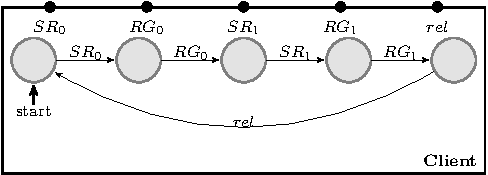
\includegraphics[scale=1.2]{compiledfigures/client-crop.pdf}
\caption{Client}
\label{fig:client}
\end{center}
\end{figure}

\begin{figure}[ht]
\begin{center}
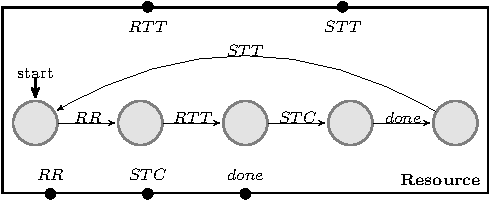
\includegraphics[scale=1.2]{compiledfigures/resource-crop.pdf}
\caption{Resource}
\label{fig:resourse}
\end{center}
\end{figure}

\begin{figure}[ht]
\begin{center}
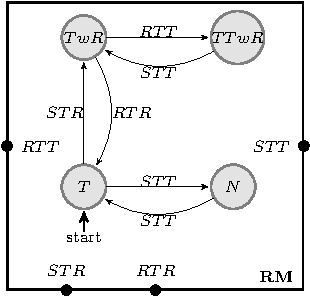
\includegraphics[scale=1.2]{compiledfigures/token-crop.pdf}
\caption{Token Resource Manager}
\label{fig:conflict-token}
\end{center}
\end{figure}

\begin{figure}[ht]
\begin{center}
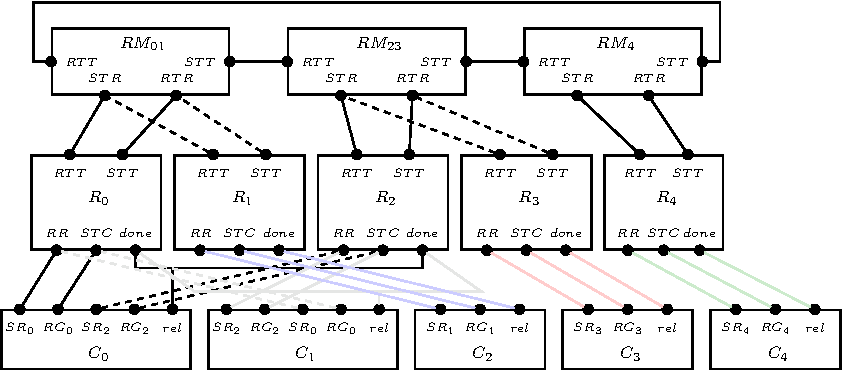
\includegraphics[scale=1.2]{compiledfigures/resourceallocation-crop.pdf}
\caption{Conflict-Resource Allocation System}
\label{fig:resourceallocation}
\end{center}
\end{figure}

We evaluated \deadlocktool{} with various configurations.
We highlight several lessons learned for specific systems as follows. 

\paragraph{Lesson 1:} 
$\LAO$ finds global and local deadlock where DFinder2 can only find global deadlock.
Consider a system with $5$ clients, $3$ tokens, and $5$ resources.
Clients request resources $\langle 0, 2\rangle, \langle 2, 0\rangle, \langle 1 \rangle, \langle 3\rangle,$ and $\langle 4\rangle$, respectively.
Resource sets $\{ 0, 1\}, \{2,3\}$ are conflicting. 
This system clearly is a global deadlock free. 
It has a local deadlock where client $C_0$ has resource $0$ and client $C_1$ has resource $2$. 
DFinder qualitatively can not detect such a local deadlock while $\LAO$ successfully does. 

\paragraph{Lesson 2:} 
$\LAO$ is more complete than both $\LLin$ and DFinder2. For example, it can detect deadlock freedom and local deadlock freedom where $\LLin$ and might fail. 
Consider a system with $5$ clients, $2$ tokens, and $5$ resources.
Clients request resources $\langle0, 2\rangle, \langle 0, 2\rangle, \langle 1 \rangle, \langle 3\rangle,$ and $\langle 4\rangle$, respectively.
Resource sets $\{ 0, 1\}, \{2,3,4\}$ are conflicting. 
This system is global and local deadlock free. 
Both DFinder2 and $\LLin$ report that the system might contain a deadlock. 
$\LAO$ successfully reports that the system is both global and local deadlock free. 

\paragraph{Lesson 3:}
Our work can be extended to detect conspiracies. 
For example, consider a system with
$5$ clients, $2$ tokens, and $5$ resources.
Clients request resources $\langle 0, 1\rangle, \langle 1, 0\rangle, \langle 2 \rangle, \langle 3\rangle,$ and $\langle 4\rangle$, respectively.
Resource sets $\{ 0, 1\}, \{2,3,4\}$ are conflicting. 
Client $C_0$ may block forever in case it acquires resource $0$ because resource $0$ is conflicting with resource $1$. 
However, it is not possible to find a deadlocked subsystem containing $C_0$ and resources $0$ and $1$ since that will also have
to include the resource manager $M_{01}$ managing conflicting resources $0$ and $1$. 
The latter can always exchange the second token with the neighboring resource managers. 

An extension of our work that consider subsystem boundaries at ports and abstracts port enablement 
conditions with free Boolean variables can help
detect such scenarios. 


\begin{table}
\centering
\begin{tabular}{| l | l | l | l |}
\hline
Size & \LAO & \LLin & D-Finder \\ \hline \hline
$10$ &          $148 s$ \\ \hline
$12$ &          $169 s$ \\ \hline
$14$ &          $189 s$ \\ \hline
$16$ &          $230 s$ \\ \hline
$18$ &          $254 s$  \\ \hline
$20$ &          $277 s$  \\ \hline 
$22$ &          $298 s$ \\ \hline 
$24$ &          $318 s$   \\ \hline 
$26$ &          $351 s$  \\ \hline 
$28$ &          $374 s$  \\ \hline
$30$ &          $430 s$   \\ \hline  
\end{tabular}
\caption{Benchmarks: Conflict-Resource Allocation}
\label{bench:resourceallocation}
\end{table}

\paragraph{Benchmarking}

We evaluated the performance of $\LAO$ on a deadlock free system with the following configuration. 
\begin{itemize}
\item $n$ clients each with $3$ states, $n$ resources each with $5$ states, and $n$ tokens,
\item Client $C_i, 0\leq i < n$ requests resource $i$, and 
\item No resources are in conflict, hence we have $n$ resource managers each with $4$ states. 
\end{itemize}

The system has a total of $4^n \times 3^n \times 5^n$ states. 
DFinder2 timed out within seven hours for $n=10$. 
%Try different combinations of partitions
$\LLin$ had to increase the subsystem up to the whole system and also timed out within seven hours for $n=10$. 
$\LAO$ was able to verify deadlock freedom. It has to check subsystems with $12$ components out of $3\times n$ components regardless of $n$. 
This resulted from inspecting subsystems corresponding to a depth $\l=2$ with $\leq 23,040,000=4^{6} \times 3^2\times 5^4$ states regardless of $n$.
The numbers in Table~\ref{bench:resourceallocation} show a linear increase in time required to check deadlock freedom 
using $\LAO$ with respect to $n$. This indicates that the number of subsystems to check is proportional to $n$. 

Our resource allocation system subsumes the token based Milner scheduler~\cite{milner} which 
is essentially a token ring with precisely one token present~\cite{AGR16}. 
The technique presented in ~\cite{AGR16} fails to prove deadlock freedom for Milner Scheduler 
because it requires a large subset of the system, 
while $\LAO$ succeeds. 


%% \clearpage
%% %%%%%%%%%%%%%%%%%%%%%%%%%%%%%%%%%%%%%%%%%%%%%%%%%%%%%%%%%%%%%%%%%%%%%%%%%%%%%%%%%%%%%%%%%%%%%%%%%%%%%
%% \section{A Condition for Deadlock Freedom in Infinite-state Systems}
%% \label{s:infinite}
%% We now present a condition for deadlock-freedom of infinite-state systems,
which can be checked using \eg an SMT solver.
$\LDFC(\BD_a)$ is implied by the conjunction of the following Hoare triples:
%
     $$\{ I \land (\land B \in C_a : ready_a(B)) \}\ a\ \{ (\land B_i \in \BD_a : noIn(B_i) \lor noOut(B_i)) \}$$ 
%
  where $I$ is any invariant, i.e., any predicate that characterizes a superset of the reachable
  states. $a'$ is an interaction whose participant set is contained in $\BD_a$, and $en(a')$ means that
  $a'$ is enabled. $noIn(B_i)$ means that $B_i$ has no incoming wait-for edges. $noOut(B_i)$ means
  that no interaction that $B_i$ readies has outgoing wait-for edges.

  Assuming that the state changes effected by interactions can be described by simple code,
  e.g., conditionals and assignments, but not loops, these triples can be mechanically reduced to
  first order formulae, e.g., using weakest preconditions \cite{Dij75}. The validity of these
  formulae can then be checked using SMT solvers.




\clearpage
%%%%%%%%%%%%%%%%%%%%%%%%%%%%%%%%%%%%%%%%%%%%%%%%%%%%%%%%%%%%%%%%%%%%%%%%%%%%%%%%%%%%%%%%%%%%%%%%%%%%%
\section{Discussion, Related Work, and Further Work}
\label{s:discussion}

\subsection{Related work.} 
The notions of wait-for-graph and supercycle \cite{AC05,AE98}
were initially defined for a shared memory program
$P = P_1 \pl \cdots \pl P_K$ in \emph{pairwise normal form}: a binary
symmettric relation $I$ specifies the directly interacting pairs
(``neighbors'') $\set{P_i, P_j}$.
If $P_i$ has neighbors $P_j$ and $P_k$, then 
the code in $P_i$ that interacts with $P_j$ is expressed separately from
the code in $P_i$ that interacts with $P_k$. 
These synchronization codes are executed synchronously and
atomically, so the grain of atomicity is proportional to the
degree of $I$.
%
Attie and Chockler \cite{AC05} give two polynomial time 
methods for (local and global) deadlock freedom.
The first checks subsystems consisting of three
processes. The second computes the wait-for-graphs of all pair subsystems $P_i \pl P_j$,
and takes their union, for all pairs
and all reachable states of each pair.
%Both methods consider in-paths and out-paths of length at most 2. The second
%method in addition considers the maximal strong components of $\mathcal{W}$. 
The first method considers only wait-for-paths of length $\le 2$. 
%due to the construction of $\mathcal{W}$, 
The second method is prone to false negatives,
%again due to $\mathcal{W}$, 
because wait-for edges generated by different states are
all merged together, which can result in spurious supercycles


G{\"o}ssler and Sifakis \cite{GS03} use a BIP-like
formalism, Interaction Models. %, which uses multiparty interactions and
%connectors to specify synchronization between components. 
They present a criterion for global deadlock freedom, based on 
%a dependency graph, which is %(like our wait-for-graph)
an and-or graph with components and constraints as the two sets of nodes. A
constraint gives the condition
under which a component is blocked. Edges are labeled with conjuncts
of the constraints.  Deadlock freedom is checked by traversing every
cycle, taking the conjunction of all the
conditions labeling its edges, and verifying that this conjunction is
always false, \ie verifying the absence of cyclical blocking.
No complexity bounds are given.
%
Martens and Majster-Cederbaum~\cite{MM12} present a polynomial time
checkable deadlock freedom condition based on structural restrictions:
``the communication structure between the components is given by a
tree.'' This restriction allows them to analyze only pair systems.
%
Aldini and Bernardo \cite{AB03} use a 
formalism based on process algebra. They check deadlock by analysing cycles in
the connections between software components, and claim scalability, but no
complexity bounds are given.

Roscoe and Dathi \cite{RD87} present several rules for freedom of global deadlock of
``triple disjoint'' (no action involves $> 2$ processes) CSP concurrent
programs. The basis for these rules is to first check that each individual process is deadlock free
(\ie the network is ``busy''), and then to define a ``variant function'' that maps the state of each
process to a partially ordered set. The first rule requires to establish that, if $P_i$ waits for
$P_j$, then the value of $P_i$'s state is greater than the value of $P_j$'s state. 
Since every process is blocked in a global deadlock, one can then construct an infinite sequence of
processes with strictly decreasing values, which are therefore all distinct. This cannot happen in a
finite network, and hence some process is not blocked.
They treat several examples, including
a self-timed systolic array (in 2 and 3 dimensions), dining philosophers, and a message switching
network.  They generalize the first rule to exploit ``disconnecting edges'' (whose removal
partitions the network into disconected components) to decompose the proof of deadlock freedom into
showing that each disconnected component is deadlock-free, and also to weaken the restriction on the
variant function so that it only has to decrease for at least one edge on each wait-for cycle.
%
Brookes and Roscoe~\cite{BR91} also provide criteria for deadlock
freedom of triple-disjoint CSP programs, and use the same technical framework as
\cite{RD87}.  However, they do not use variant functions, but show that, in a busy
network, a deadlock implies the existence of a wait-for cycle. They give many examples,
and demonstrate the absence of wait-for cycles in each example, by ad-hoc
reasoning. Finally, they give a deadlock freedom rule that exploits disconnecting edges,
similar to that of \cite{RD87}.
%
In both of these papers, the wait-for relations are defined by examining a pair of processes
at a time: $P_i$ waits for $P_j$ iff $P_i$ offers an action to $P_j$ which $P_j$ is
not willing to participate in.

Martin \cite{Ma96} applies the results in \cite{RD87} and \cite{BR91} to formulate deadlock-freedom design rules for several classes of CSP concurrent
programs: cyclic processes, client-server protocols, and resource allocation protocols. He also introduces the notion of ``state dependence digraph''
(SDD), whose nodes are local states of individual proceses, and whose edges are wait-for relations between processes in particular local states. An
acyclic SDD implies deadlock-freedom. A cyclic SDD does not imply deadlock, however, since the cycle may be ``spurious'': the local states along the
cycle may not be reachable at the same time, and so the cycle cannot give rise to an actual deadlock during execution. Hence the SDD approach cannot
deal with ``non-hereditary'' deadlock freedom, \ie a deadlock free system that contains a deadlock prone subsystem. Consider, \eg, the dining
philosophers with a butler solution; removing the butler leaves a deadlock prone subsystem.
%
Antonio \etal \cite{AGR16} takes the SDD approach and improves its accuracy by checking for mutual reachability of pairs of local states, and also
eliminating local states and pairs of local states, where action enablement can be verified locally.



We compared our implementation \ldfctool to D-Finder 2~\cite{DFinder2}. D-Finder 2
computes a finite-state abstraction for each component, which it uses
to compute a global invariant $I$. It then checks if $I$ 
implies deadlock freedom.  Unlike \ldfctool, D-Finder 2 
handles infinite state systems.
However, \ldfctool had superior running time for
dining philosophers and gas station (both finite-state).


All the above methods (except Attie and Chockler \cite{AC05}) verify global (and not
local) deadlock-freedom.  Our method verifies local deadlock-freedom, which subsumes 
global deadlock-freedom as a special case.
Also, our approach makes no
structural restriction at all on the system being checked for deadlock.  Our method checks
for the absence of supercycles, which are a sound and complete characterization of
deadlock, and the \LAO condition is complete \wrt the occurrence of a supercycle wholly
within the subsystem being checked. 
Hence the only source of incompleteness in our method is that of computational
limitation: if the subsystem being checked becomes too large before 
the \LAO condition is verified. If compuational resources are not exhausted, then our
method can keep checking until the subsystem being checked is the entire system, at which
point \LAO concides with \GAO, which is sound and complete for local deadlock
(\prop{scViol-iff-notInSC}, \defn{formation.violation}, and \defn{global.ANDOR-cond}).






\subsection{Discussion}
Our approach has the following advantages:
\begin{description}

\item[Local and global deadlock] Our method shows that no subset of processes
  can be deadlocked, \ie absence of both local and global deadlock. 

\item[Check works for realistic formalism]   By applying the approach to BIP, we
provide an efficient deadlock-freedom check within a formalism from
which efficient distributed implementations can be generated
\cite{BonakdarpourBJQS10b}.  

\item[Locality] If a component $B_i$ is modified, or is added to an
  existing system, then $\LDFC(a, \l)$ only has to
  be re-checked for $B_i$ and components within distance $\l$ of $B_i$.
  A condition whose evaluation considers the entire
  system at once, \eg \cite{AB03,DFinder2,GS03}
  would have to be re-checked for the entire system. 

\item[Easily parallelizable] Since the checking of each subsystem $\dsk{a}{\l}$
  is independent of the others, the checks can be carried out in parallel. Hence
  our method can be easily parallelized and distributed, for speedup, if needed.
  Alternatively, performing the checks sequentially
  minimizes the amount of memory needed. 

\item[Framework aspect] Supercycles and in/out-depth provide a \emph{framework} for
  deadlock-freedom. Conditions more general and/or discriminating than
  the one presented here 
  should be devisable in this framework. This is a topic for future work.

\end{description}


\subsection{Further work.} 
Our implementation uses explicit state enumeration. % to evaluate $\LDFC(a, \l)$.
Using BDD's may improve the running time 
when $\LDFC(a, \l)$ holds only for large $\l$.
%, since the time to check $\LDFC(a, \l)$ grows exponentialy with $\l$, in general.
%
An enabled port $p$ enables all interactions containing $p$.
Deadlock-freedom conditions based on ports could exploit
this interdepence among interaction enablement.
%
Our implementation should produce \emph{counterexamples} when a system
fails to satisfy $\LDFC(a, \l)$.
%
\emph{Design rules} for ensuring $\LDFC(a, \l)$ will help users to
produce deadlock-free systems, and also to interpret counterexamples.
%
A \emph{fault} may create a deadlock,  \ie a supercycle, by creating 
wait-for-edges that would not normally arise.
Tolerating a fault that creates up to $f$ such spurious wait-for-edges 
requires that there do not arise during normal
(fault-free) operation subgraphs of $\wfg{B}{s}$ that can be made into a
supercycle by adding $f$ edges. 
We will investigate criteria for preventing formation of such subgraphs.
%
Methods for evaluating $\LDFC(a, \l)$ on \emph{infinite state} systems will be
devised, \eg, by extracting proof obligations and verifying using SMT solvers.
%This verifies local deadlock freedom, which, unlike global deadlock freedom,
%cannot be succinctly expressed in first order logic.
%
We will extend our method to \emph{Dynamic BIP},
\cite{DBLP:conf/soco/BozgaJMS12}, where participants can add and remove
interactions at run time.






%%%%%%%%%%%%%%%%%%%%%%%%% BIBLIOGRAPHY %%%%%%%%%%%%%%%%%%%%%%%
\bibliographystyle{plain}
\bibliography{biblio}


%%% alternative biblio
%\bibliographystyle{alpha}
%\bibliography{Bibfiles/ABBREV,Bibfiles/DIST,Bibfiles/IOAUT,Bibfiles/MODEL,Bibfiles/SYNTH,Bibfiles/LOGIC,Bibfiles/MOBILE}


\end{document}


















